\documentclass[aspectratio=169,xcolor=dvipsnames]{beamer}

\usetheme{Warsaw}
%\usepackage{appendixnumberbeamer}
%\usefonttheme{serif}
\usefonttheme[onlymath]{serif} %options:stillsansseriflarge,stillsansserifmath

\usepackage[numbers,sort&compress]{natbib}
\usepackage{booktabs}
\usepackage[scale=2]{ccicons}
\usepackage{relsize}
\usepackage{amsmath}
\usepackage{bm}
\usepackage{xspace}
\usepackage[normalem]{ulem}
\usepackage{braket}
\usepackage[thicklines]{cancel}
\usepackage{varwidth}
\usepackage[export]{adjustbox}
\usepackage{listings}
\usepackage{wasysym}
\usepackage{tabu}
\usepackage{relsize}
\usepackage{caption}
\usepackage{tcolorbox}
\usepackage{siunitx}
\usepackage{lmodern}
\usepackage{float}% If comment this, figure moves to Page 2
\usepackage{tabu}
\usepackage{multirow}
\usepackage{array}
%\newcommand{\themename}{\textbf{\textsc{metropolis}}\xspace}

\title{csv ratio}
% \subtitle{Subtítulo}
% \date{\today}
\date{}
\author{Shuo Jia}
%\institute{UFPR - Disciplina - Semestre}
% \titlegraphic{\hfill\includegraphics[height=1.5cm]{logo.pdf}}

\begin{document}

\maketitle

%\begin{frame}{Table of contents}
%  \setbeamertemplate{section in toc}[sections numbered]
%  \tableofcontents[hideallsubsections]
%\end{frame}
%\section{Introduction}

\begin{frame}{CSV kinematics}
\begin{columns}
\begin{column}[T]{0.5\textwidth}
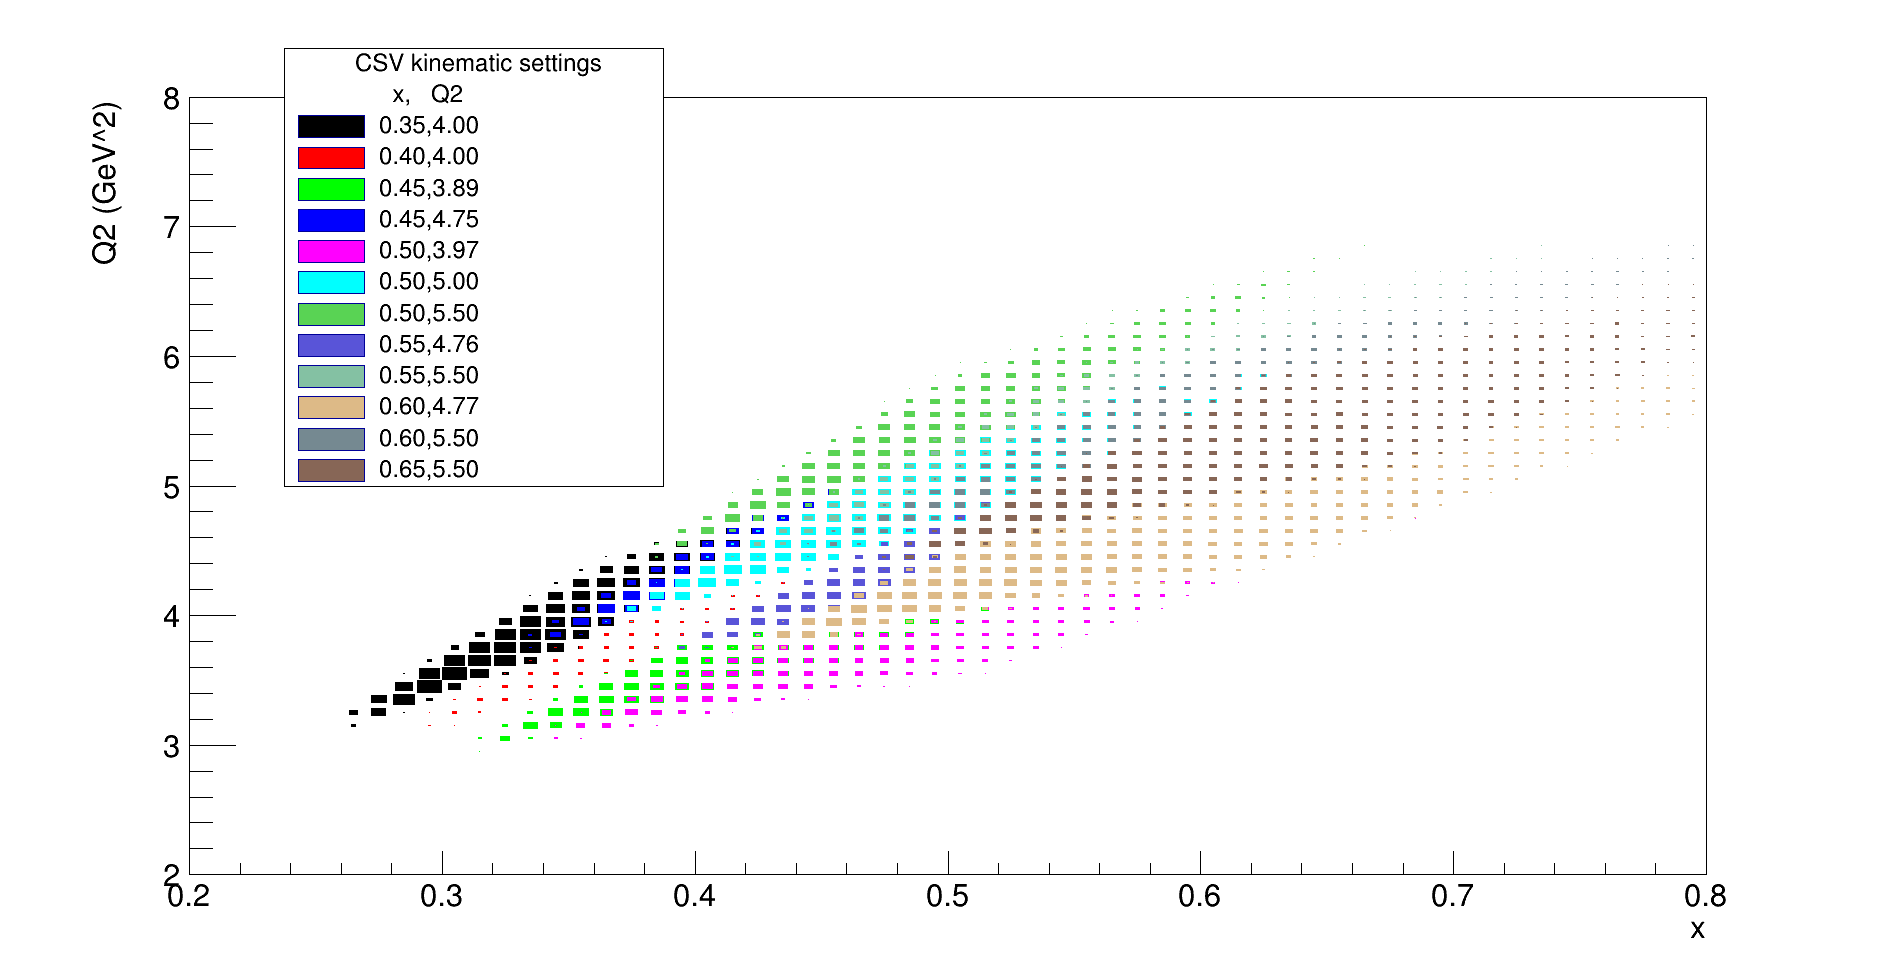
\includegraphics[width = 0.9\textwidth]{results/yield/kin_x_Q2_pos.png}
\end{column}
\begin{column}[T]{0.5\textwidth}
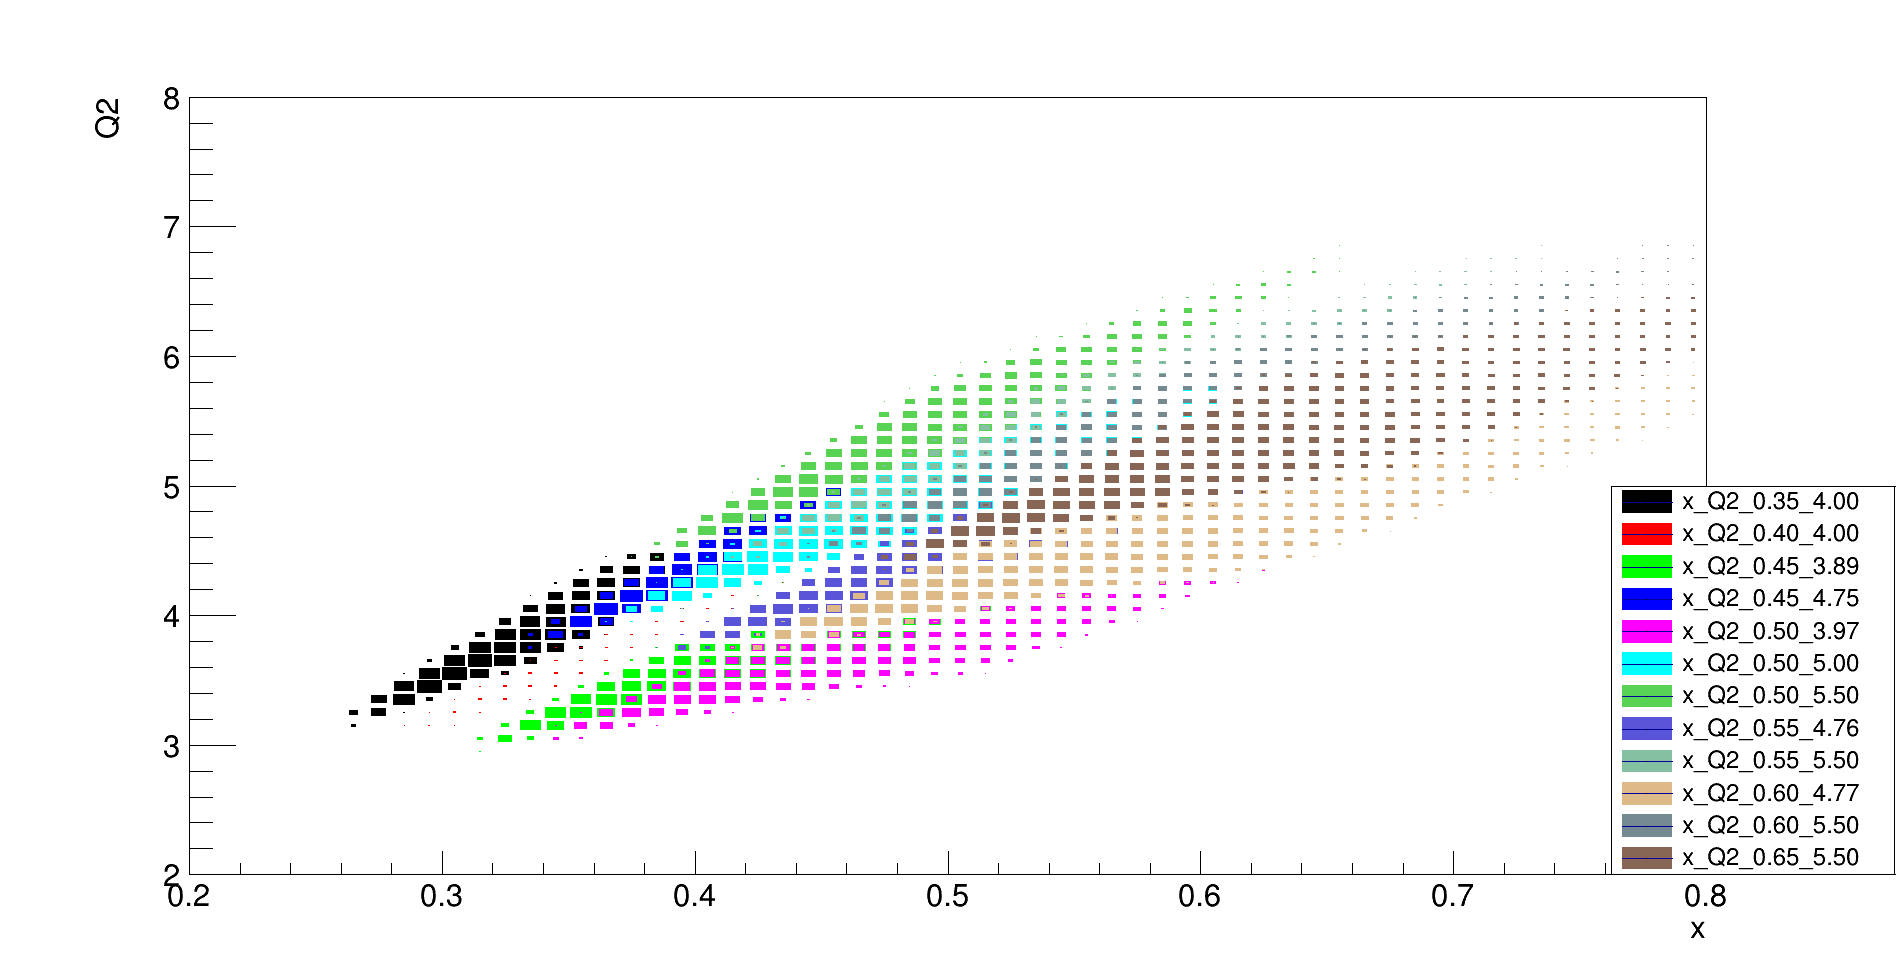
\includegraphics[width = 0.9\textwidth]{results/yield/kin_x_Q2_neg.png}
\end{column}
\end{columns}
\end{frame}
\begin{frame}{}
cuts for raw yield(blue for pions, yellow for accidentals) and raw yield ratio: 
    \begin{itemize}
        \item cointime
        \item rftime pid
        \item HMS cherenkov, calorimeter,delta,xptar
        \item SHMS aero,calorimeter,delta,xptar
    \end{itemize}
\\
corrected yield ratio:
\begin{itemize}
    \item Tracking efficiency
    \item rftiming cut, efficiency and contamination
\end{itemize}
\end{frame}
\begin{frame}{corrected yield}
\begin{columns}
\begin{column}[T]{0.25\textwidth}
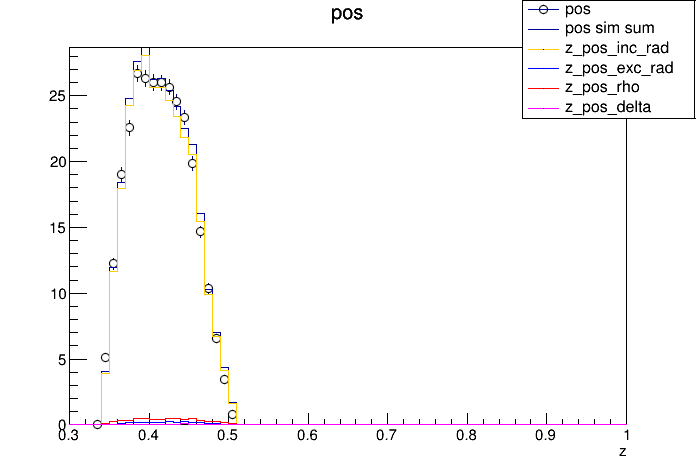
\includegraphics[width = \textwidth]{results/yield/statistics_corr/yield_x_Q2_z_0.35_4.000_0.40_pos.png}
\end{column}
\begin{column}[T]{0.25\textwidth}
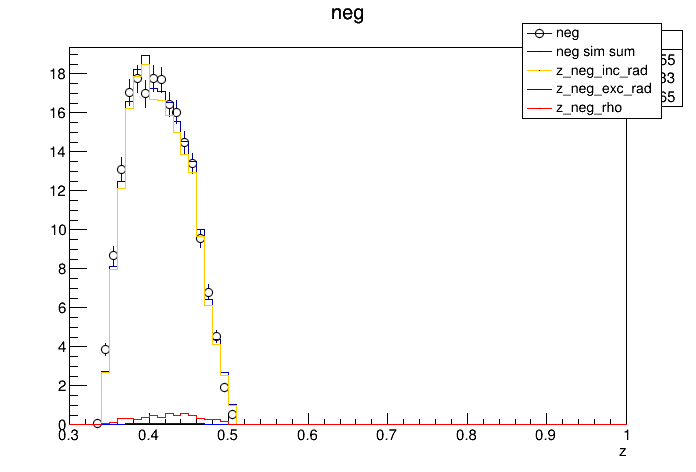
\includegraphics[width = \textwidth]{results/yield/statistics_corr/yield_x_Q2_z_0.35_4.000_0.40_neg.png}
\end{column}
\begin{column}[T]{0.25\textwidth}
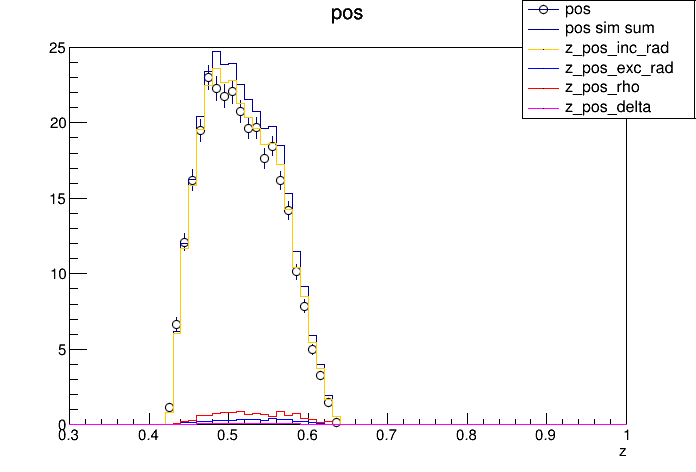
\includegraphics[width = \textwidth]{results/yield/statistics_corr/yield_x_Q2_z_0.35_4.000_0.50_pos.png}
\end{column}
\begin{column}[T]{0.25\textwidth}
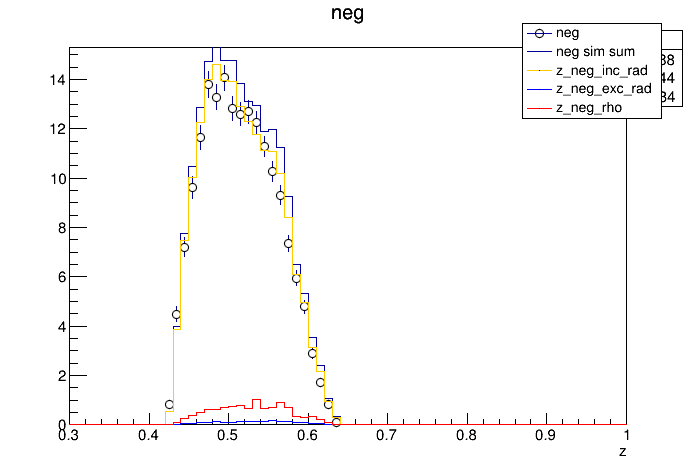
\includegraphics[width = \textwidth]{results/yield/statistics_corr/yield_x_Q2_z_0.35_4.000_0.50_neg.png}
\end{column}
\end{columns}
\begin{columns}
\begin{column}[T]{0.25\textwidth}
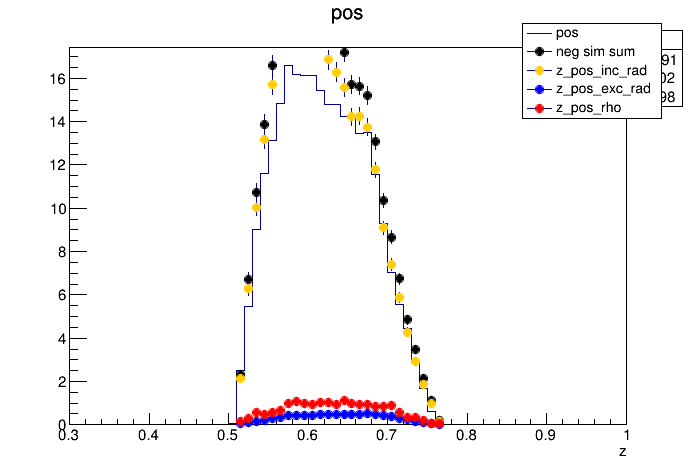
\includegraphics[width = \textwidth]{results/yield/statistics_corr/yield_x_Q2_z_0.35_4.000_0.60_pos.png}
\end{column}
\begin{column}[T]{0.25\textwidth}
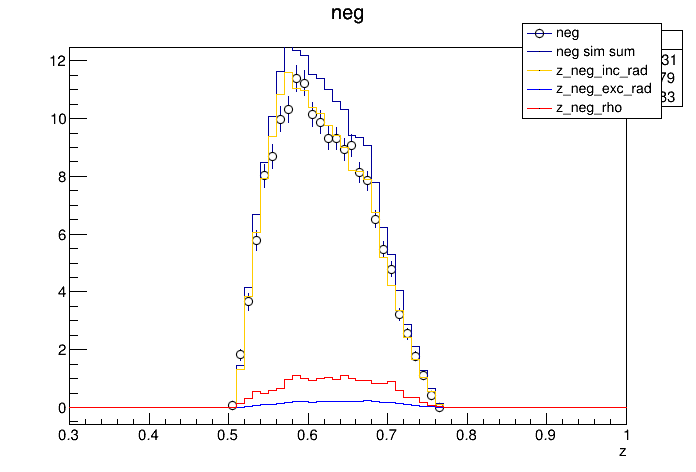
\includegraphics[width = \textwidth]{results/yield/statistics_corr/yield_x_Q2_z_0.35_4.000_0.60_neg.png}
\end{column}
\begin{column}[T]{0.25\textwidth}
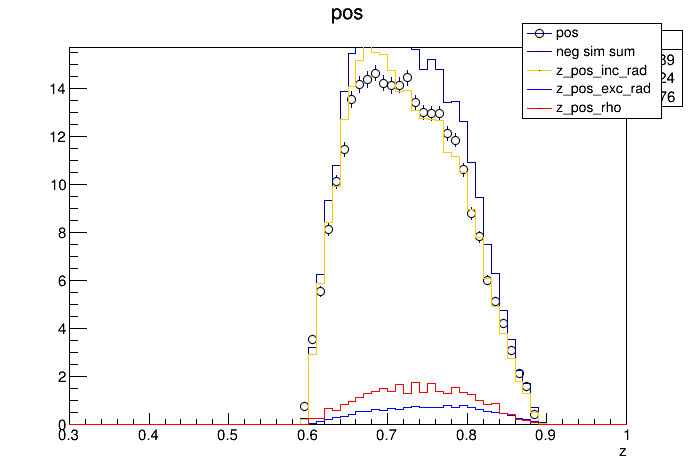
\includegraphics[width = \textwidth]{results/yield/statistics_corr/yield_x_Q2_z_0.35_4.000_0.70_pos.png}
\end{column}
\begin{column}[T]{0.25\textwidth}
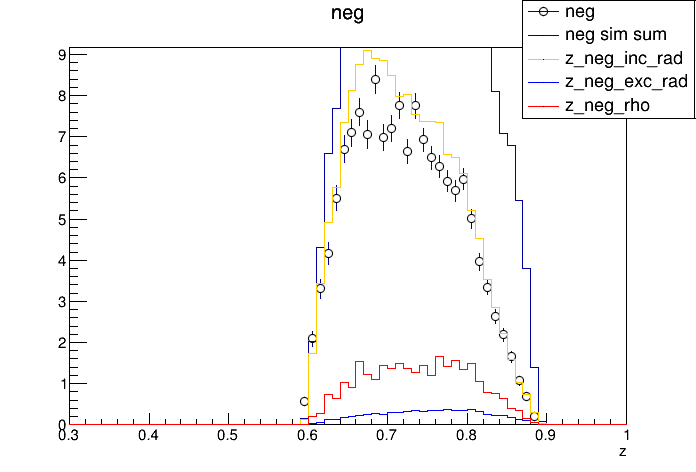
\includegraphics[width = \textwidth]{results/yield/statistics_corr/yield_x_Q2_z_0.35_4.000_0.70_neg.png}
\end{column}
\end{columns}
\end{frame}
\begin{frame}{raw yield ratio}
\begin{columns}
\begin{column}[T]{0.5\textwidth}
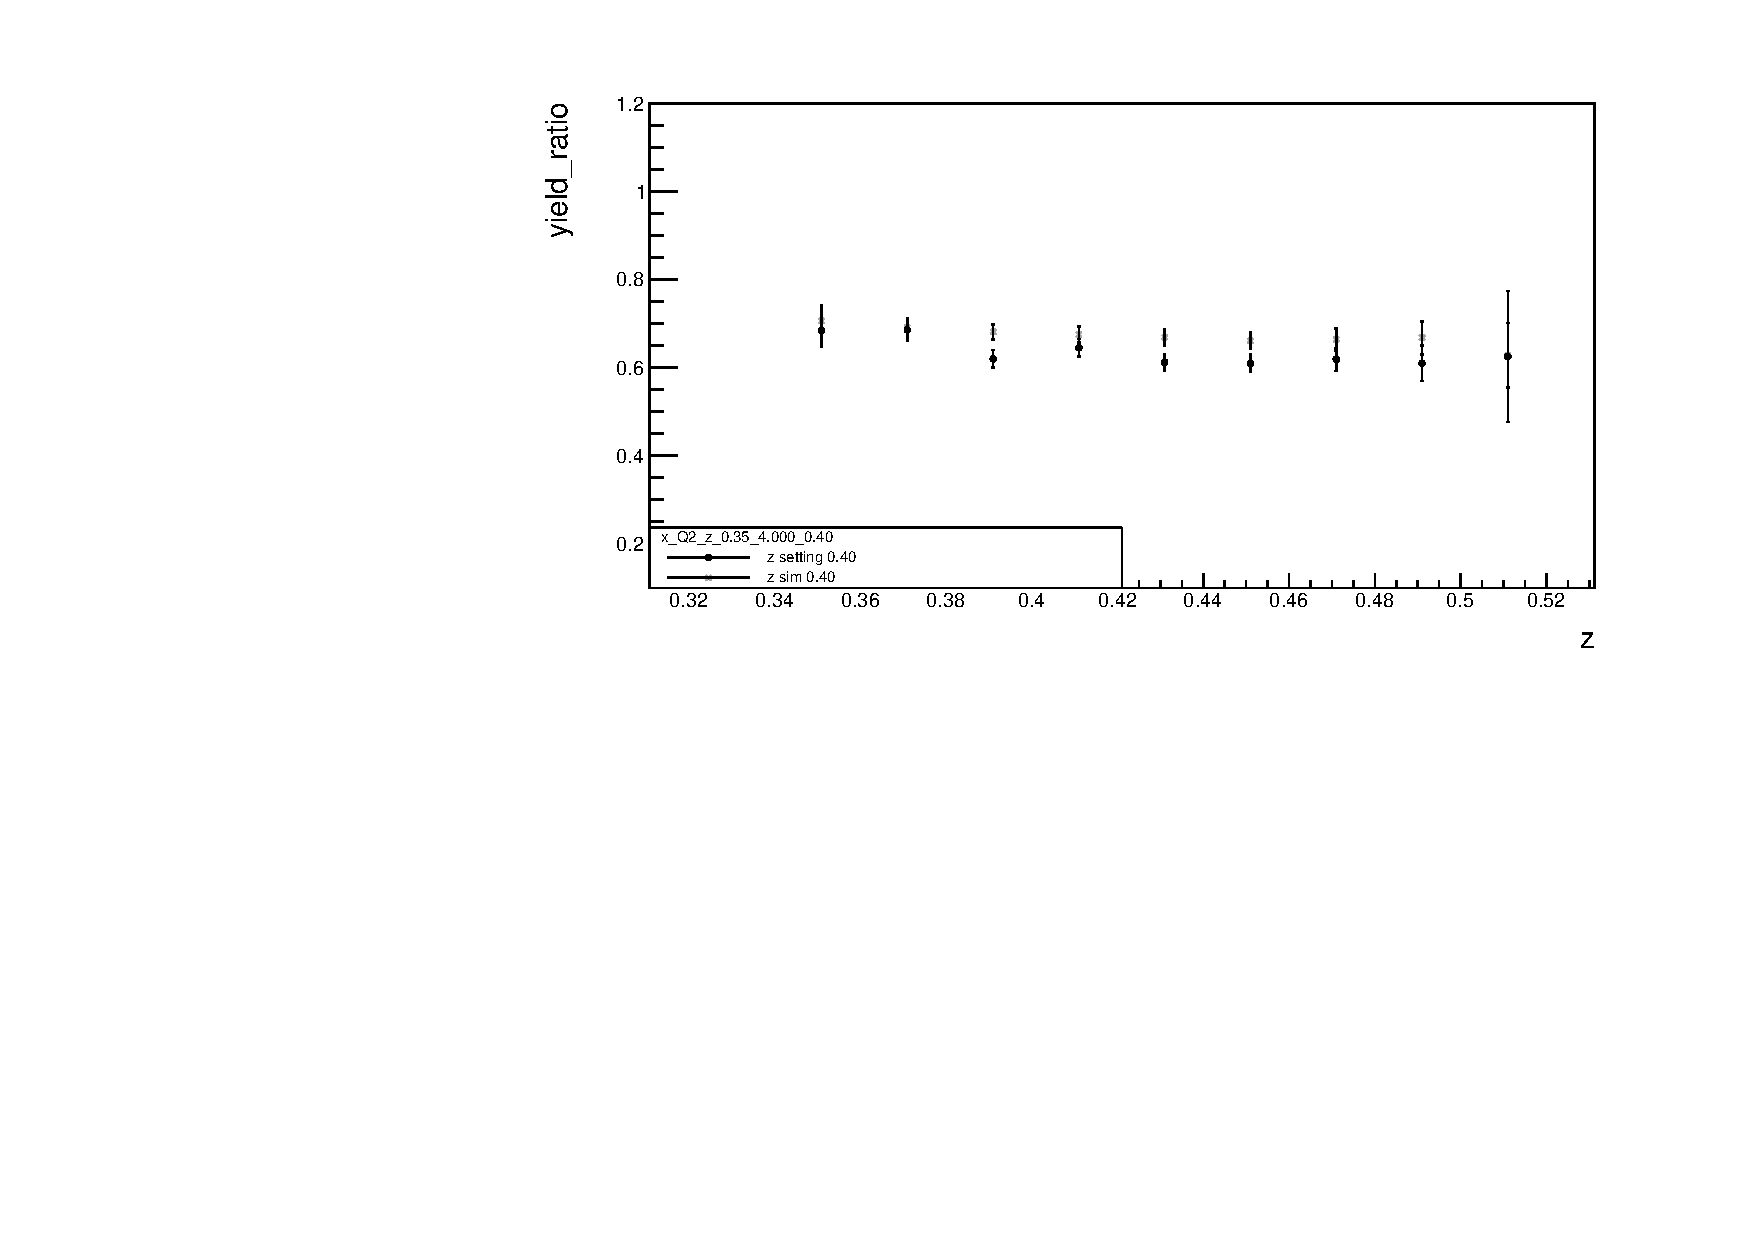
\includegraphics[width = 0.9\textwidth]{results/yield/statistics/x_Q2_z_0.35_4.000_0.40_ratio.pdf}
\end{column}
\begin{column}[T]{0.5\textwidth}
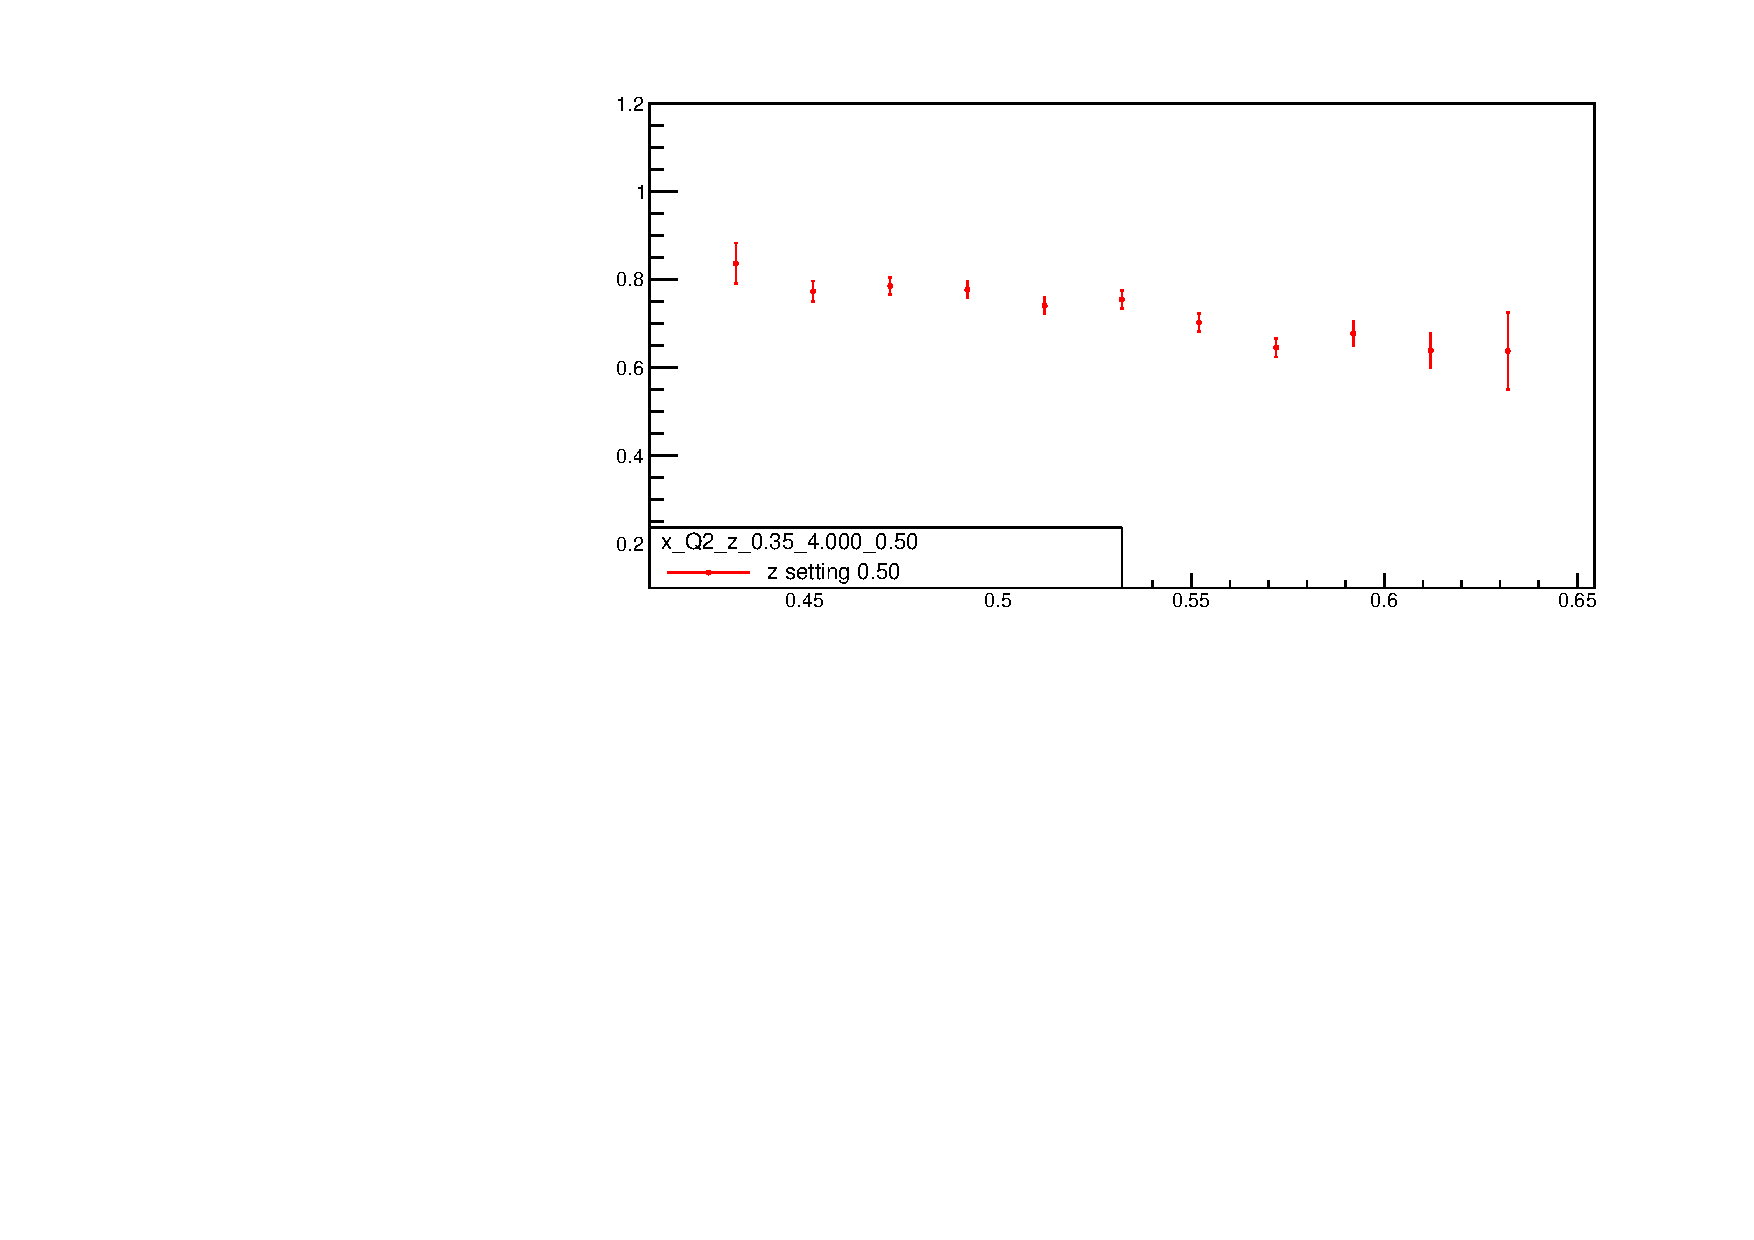
\includegraphics[width = 0.9\textwidth]{results/yield/statistics/x_Q2_z_0.35_4.000_0.50_ratio.pdf}
\end{column}
\end{columns}
\begin{columns}
\begin{column}[T]{0.5\textwidth}
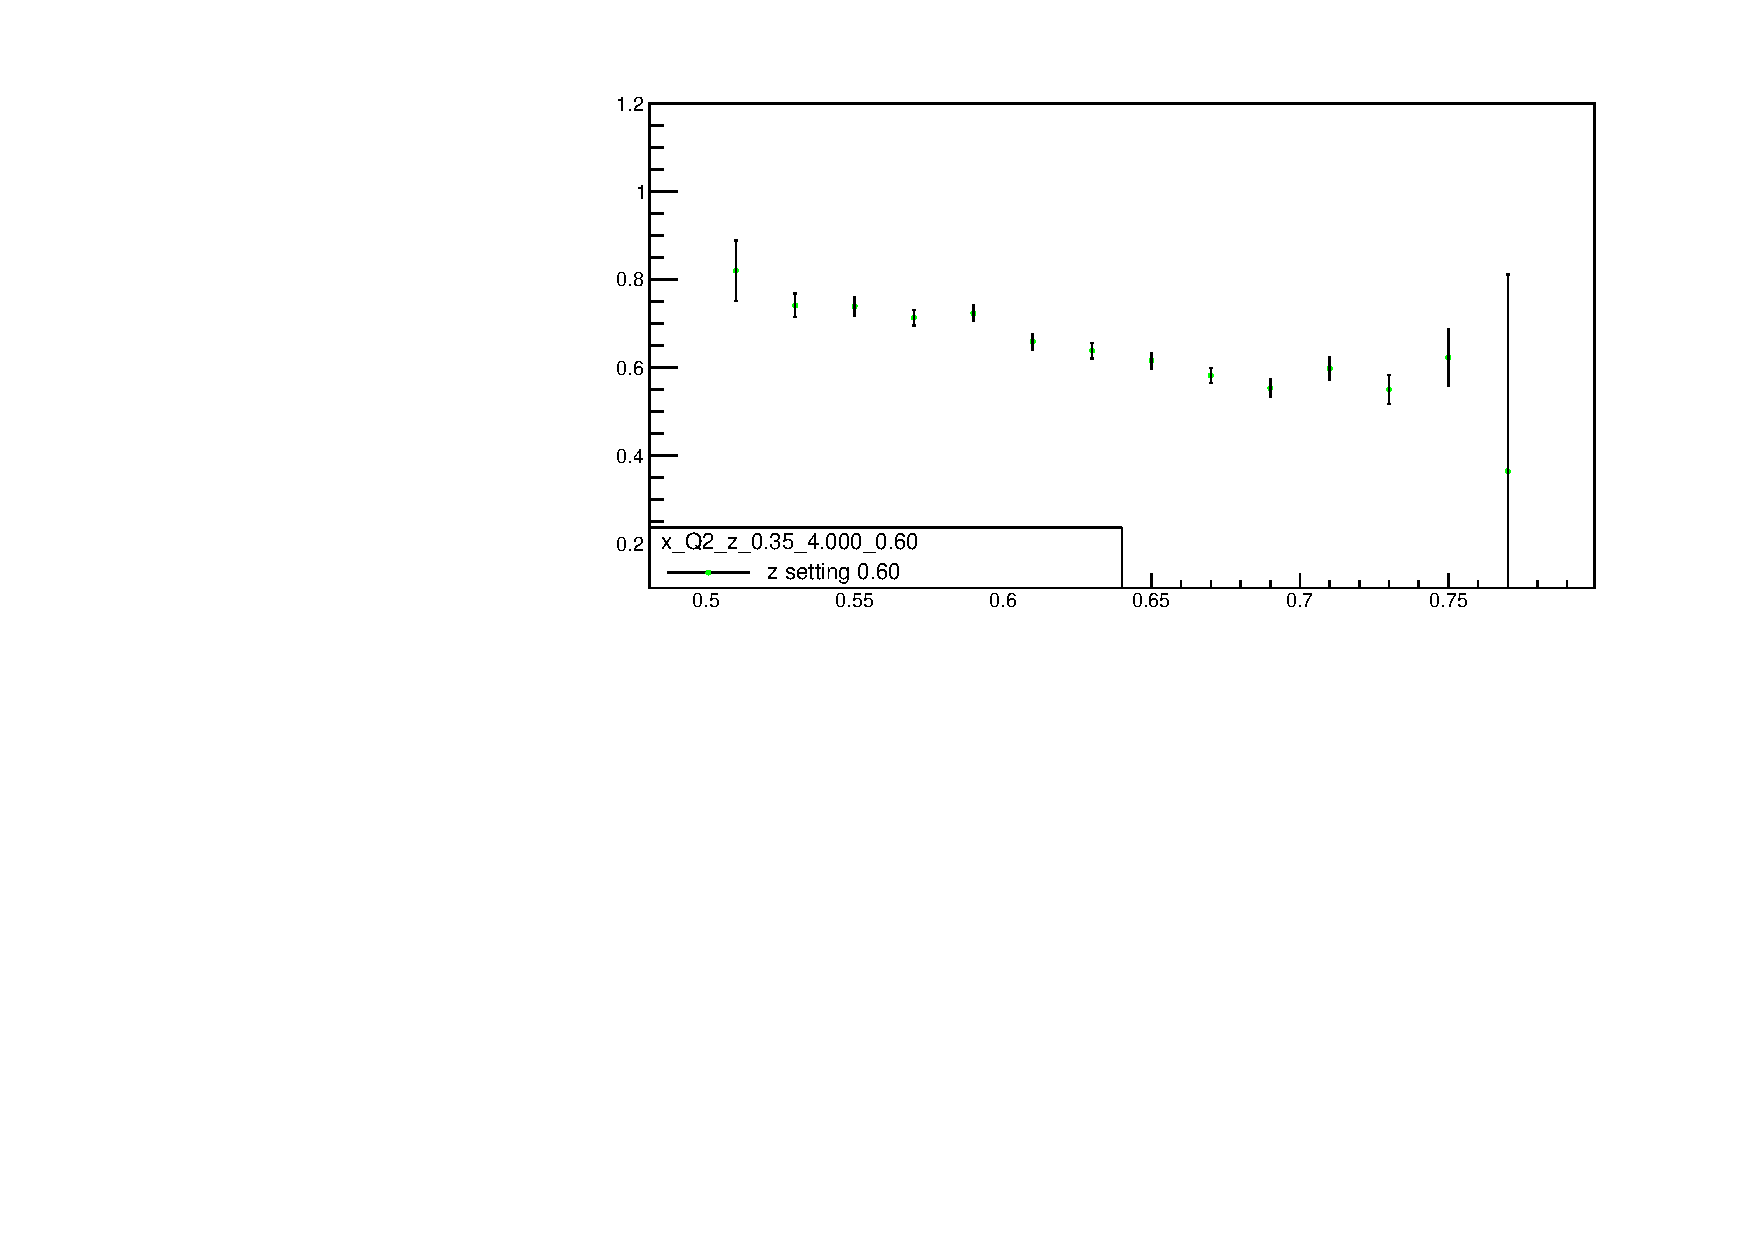
\includegraphics[width = 0.9\textwidth]{results/yield/statistics/x_Q2_z_0.35_4.000_0.60_ratio.pdf}
\end{column}
\begin{column}[T]{0.5\textwidth}
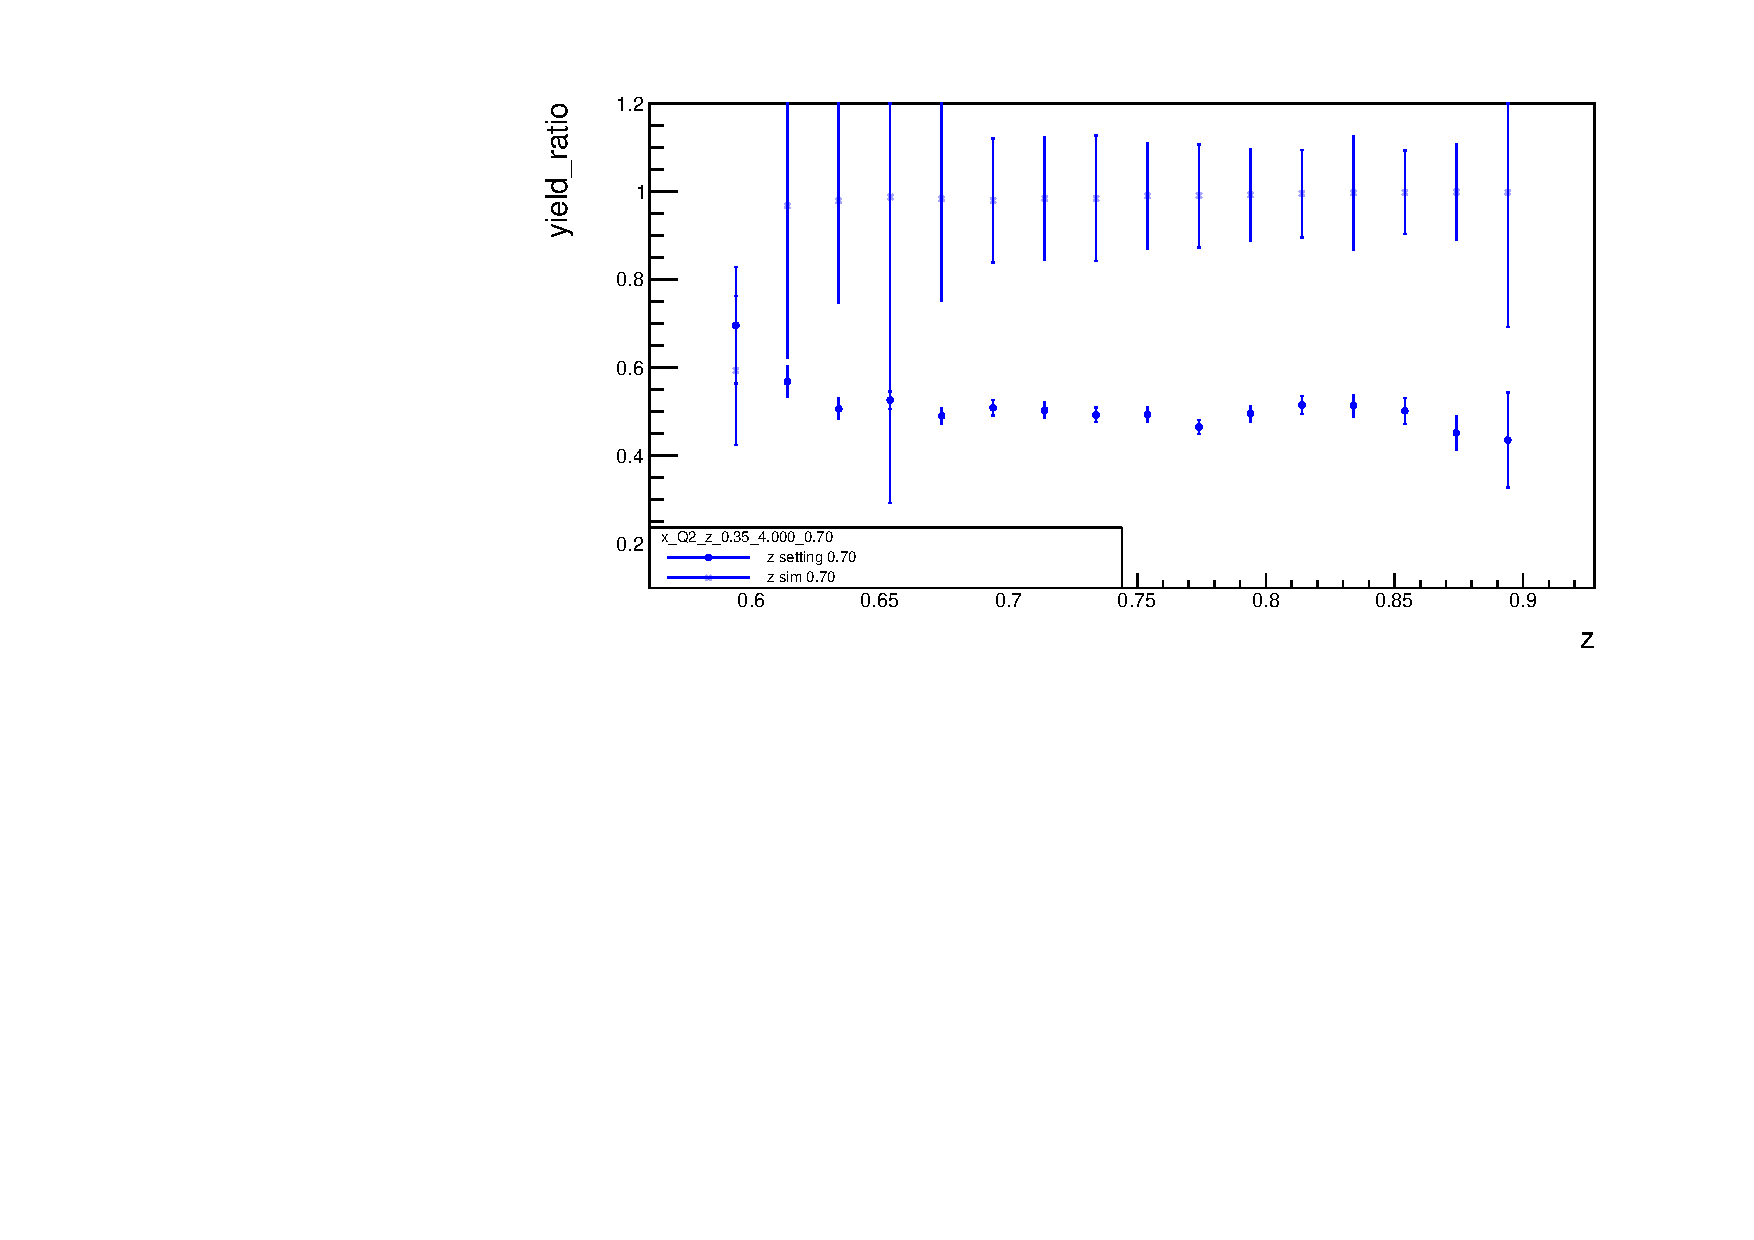
\includegraphics[width = 0.9\textwidth]{results/yield/statistics/x_Q2_z_0.35_4.000_0.70_ratio.pdf}
\end{column}
\end{columns}
\end{frame}
\begin{frame}{TE,pi eff, pi purity corrected yield ratio}
\begin{columns}
\begin{column}[T]{0.5\textwidth}
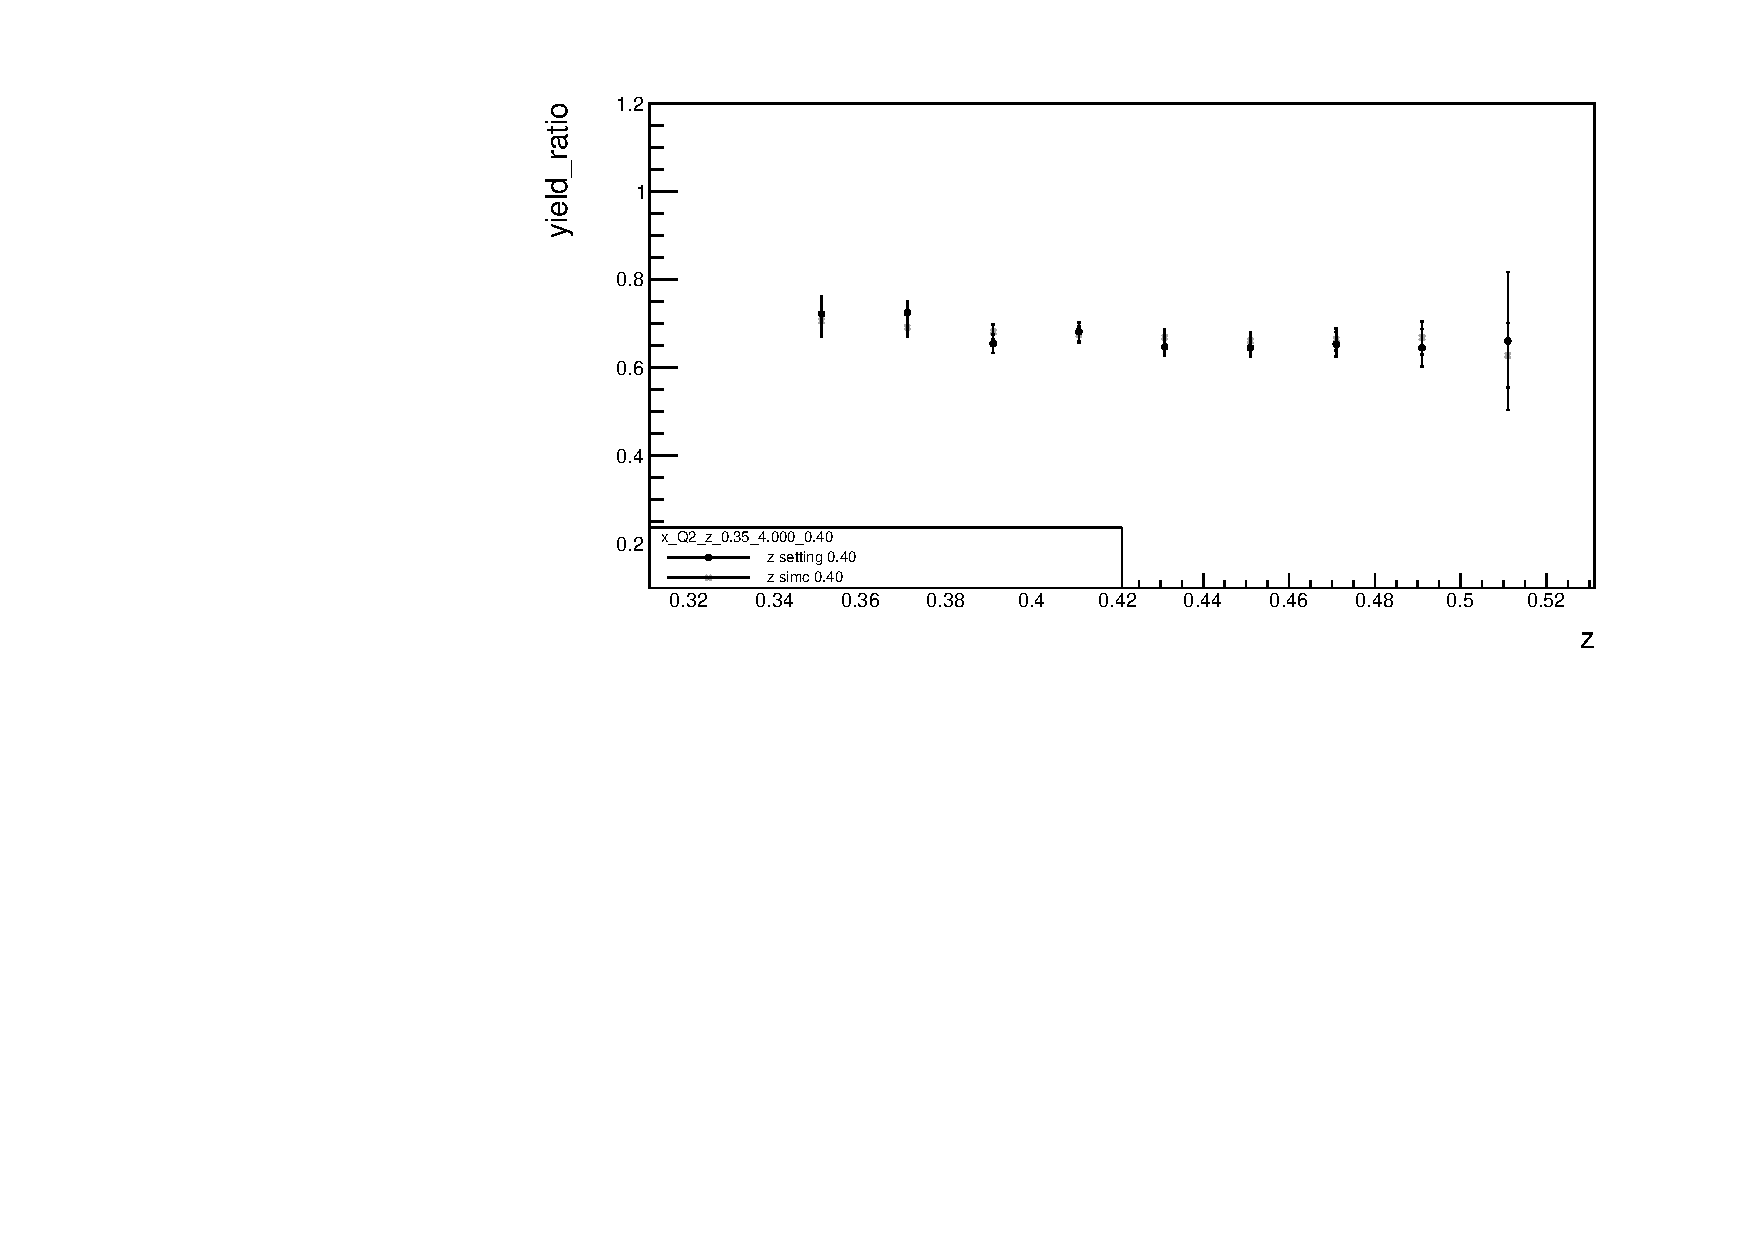
\includegraphics[width = 0.9\textwidth]{results/yield/statistics_corr/x_Q2_z_0.35_4.000_0.40_ratio.pdf}
\end{column}
\begin{column}[T]{0.5\textwidth}
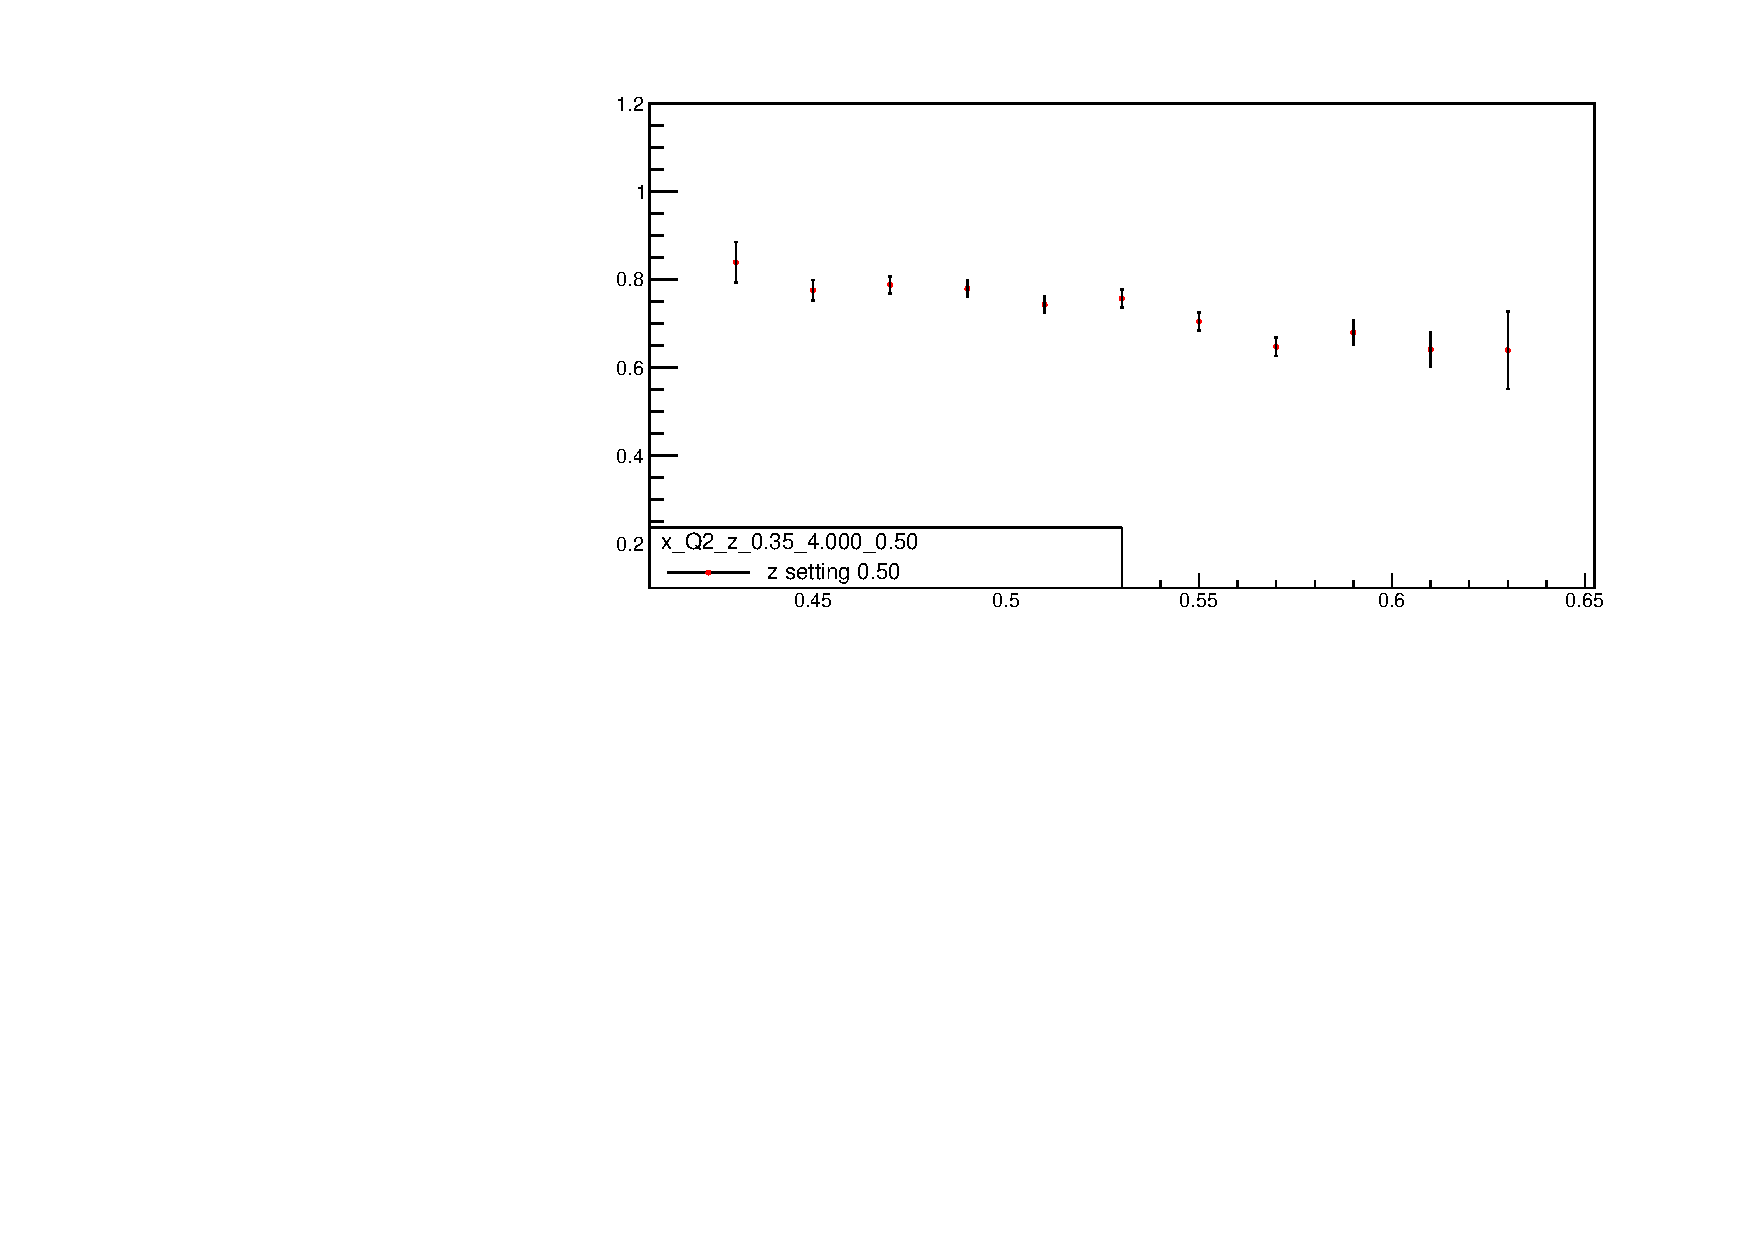
\includegraphics[width = 0.9\textwidth]{results/yield/statistics_corr/x_Q2_z_0.35_4.000_0.50_ratio.pdf}
\end{column}
\end{columns}
\begin{columns}
\begin{column}[T]{0.5\textwidth}
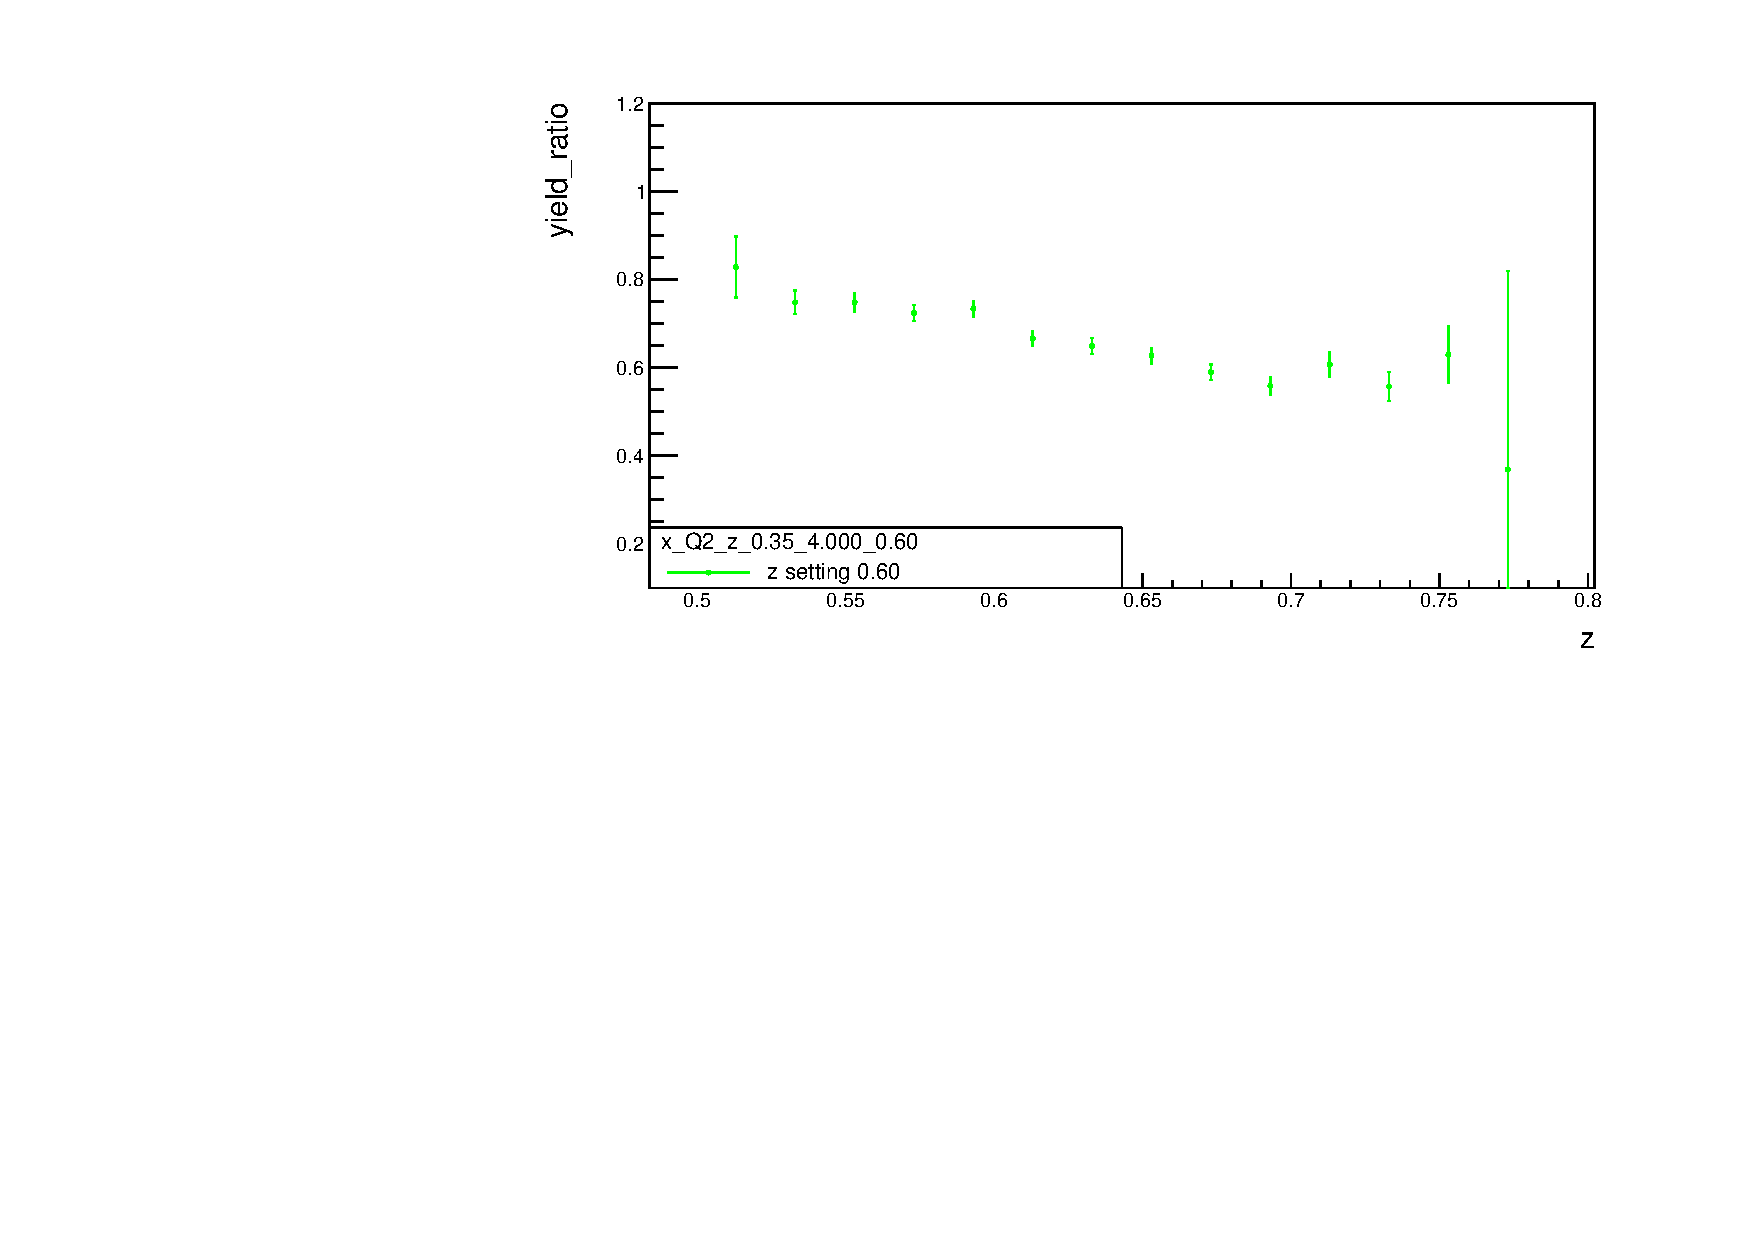
\includegraphics[width = 0.9\textwidth]{results/yield/statistics_corr/x_Q2_z_0.35_4.000_0.60_ratio.pdf}
\end{column}
\begin{column}[T]{0.5\textwidth}
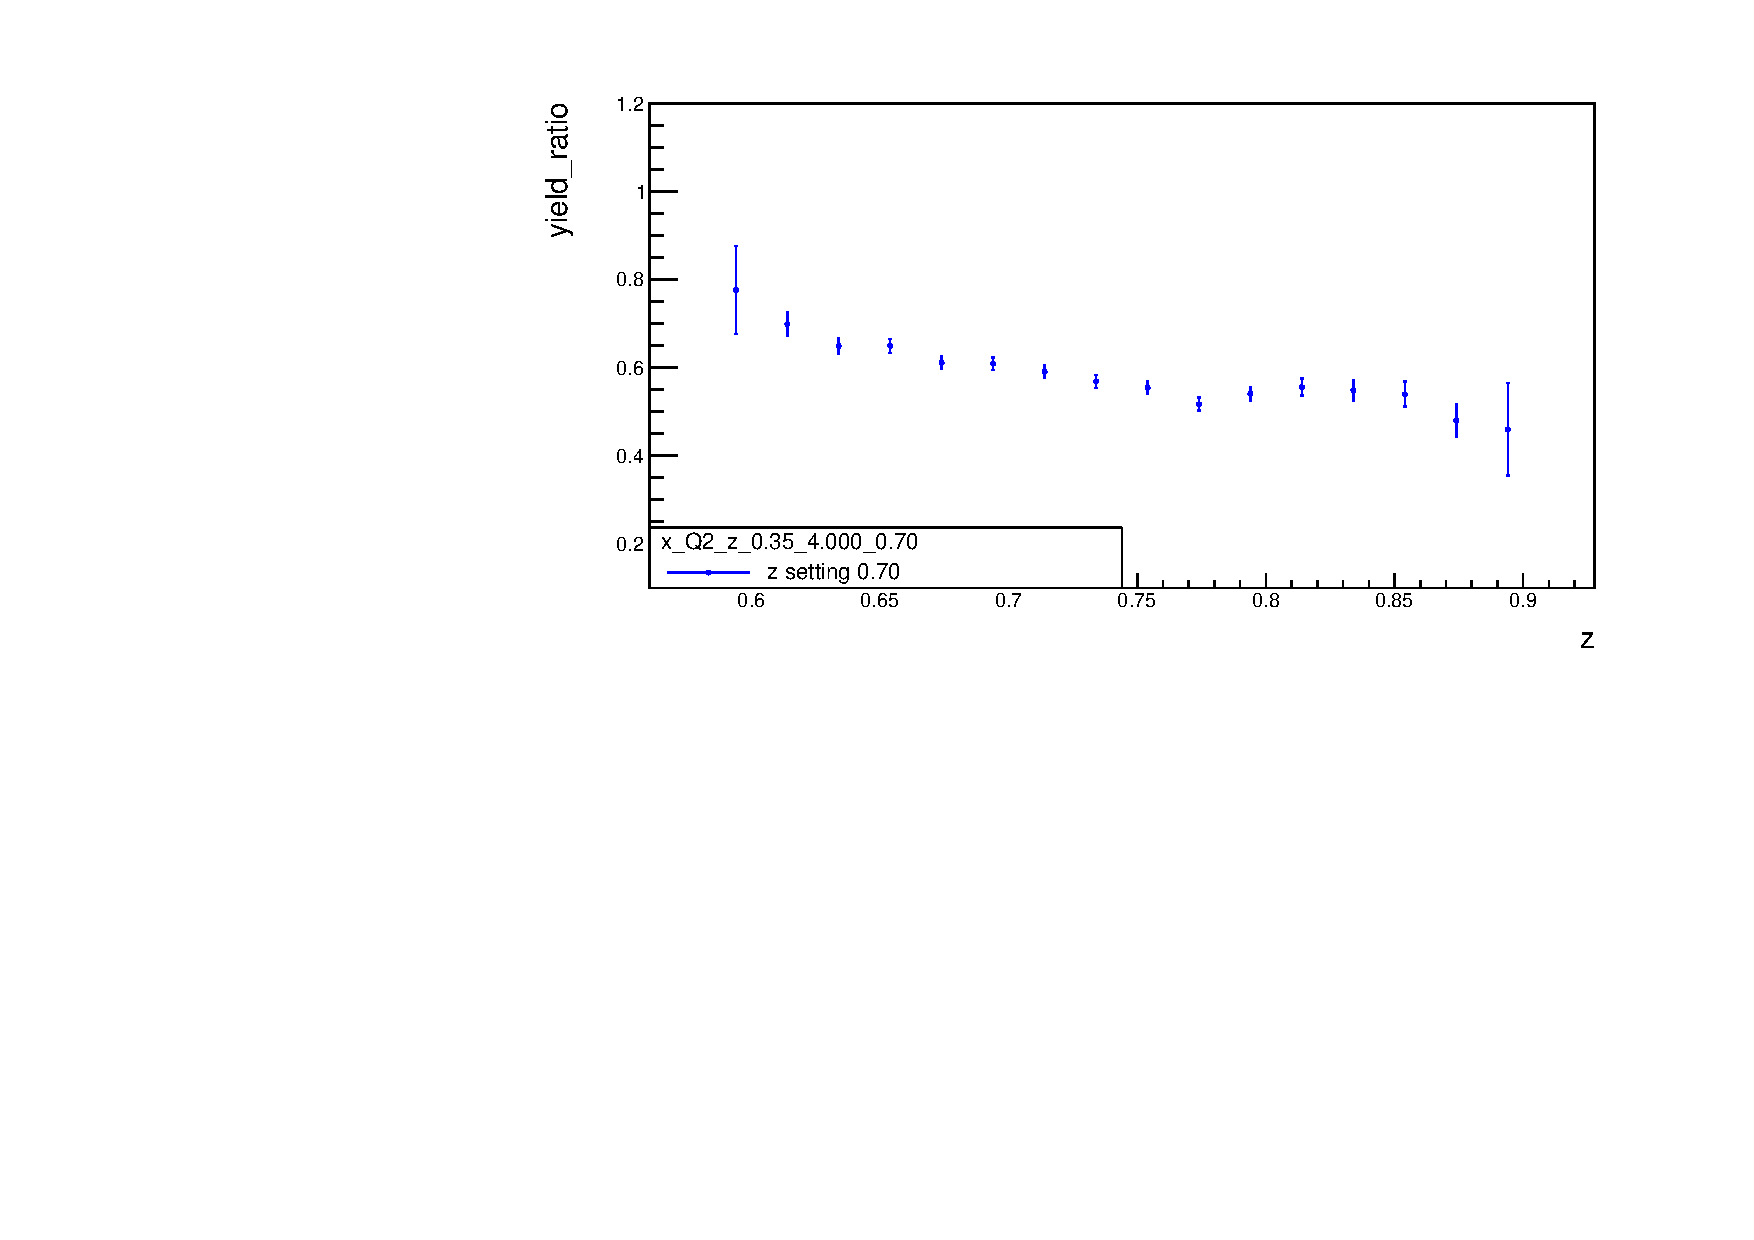
\includegraphics[width = 0.9\textwidth]{results/yield/statistics_corr/x_Q2_z_0.35_4.000_0.70_ratio.pdf}
\end{column}
\end{columns}
\end{frame}
\begin{frame}{raw yield ratio}
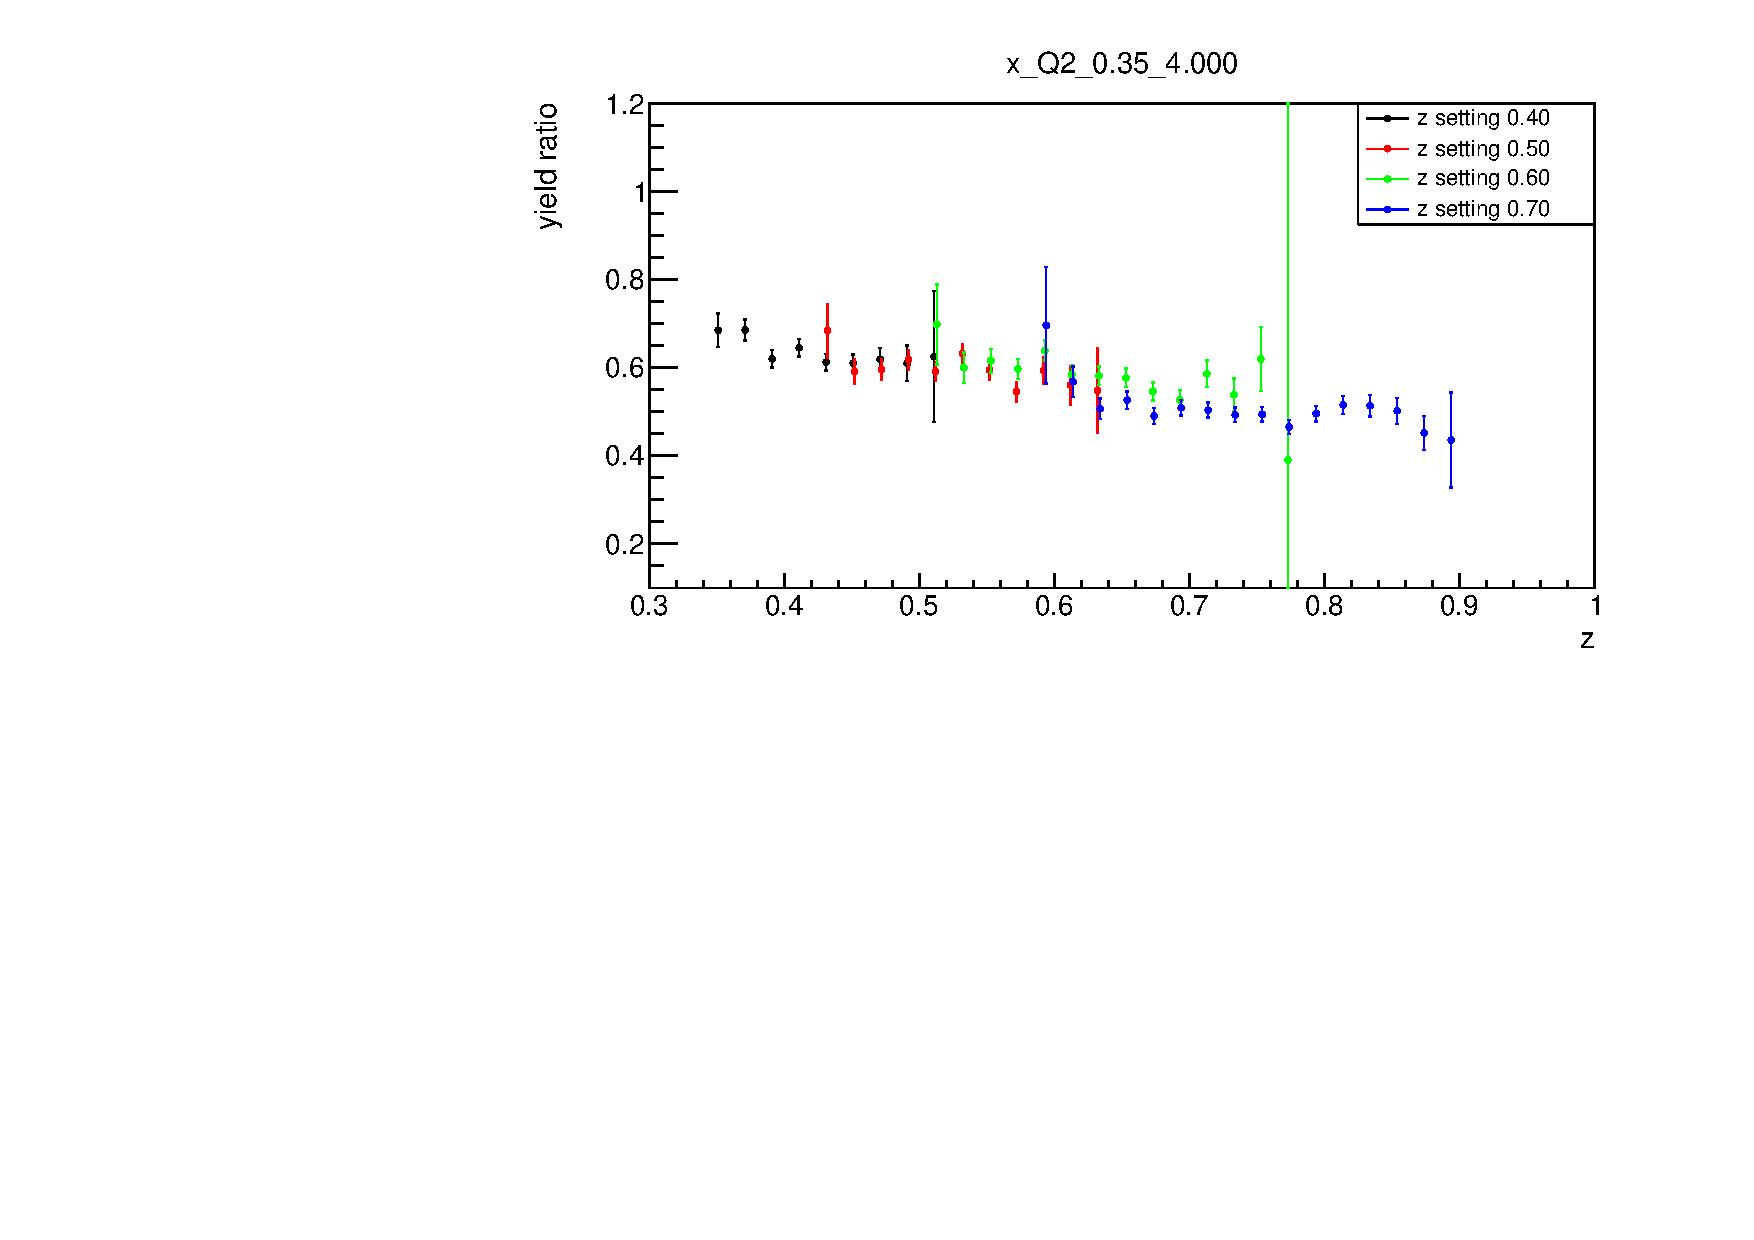
\includegraphics[width = 0.9\textwidth]{results/yield/statistics/x_Q2_0.35_4.000_ratio.pdf}
\end{frame}
\begin{frame}{TE,pi eff, pi purity corrected yield ratio}
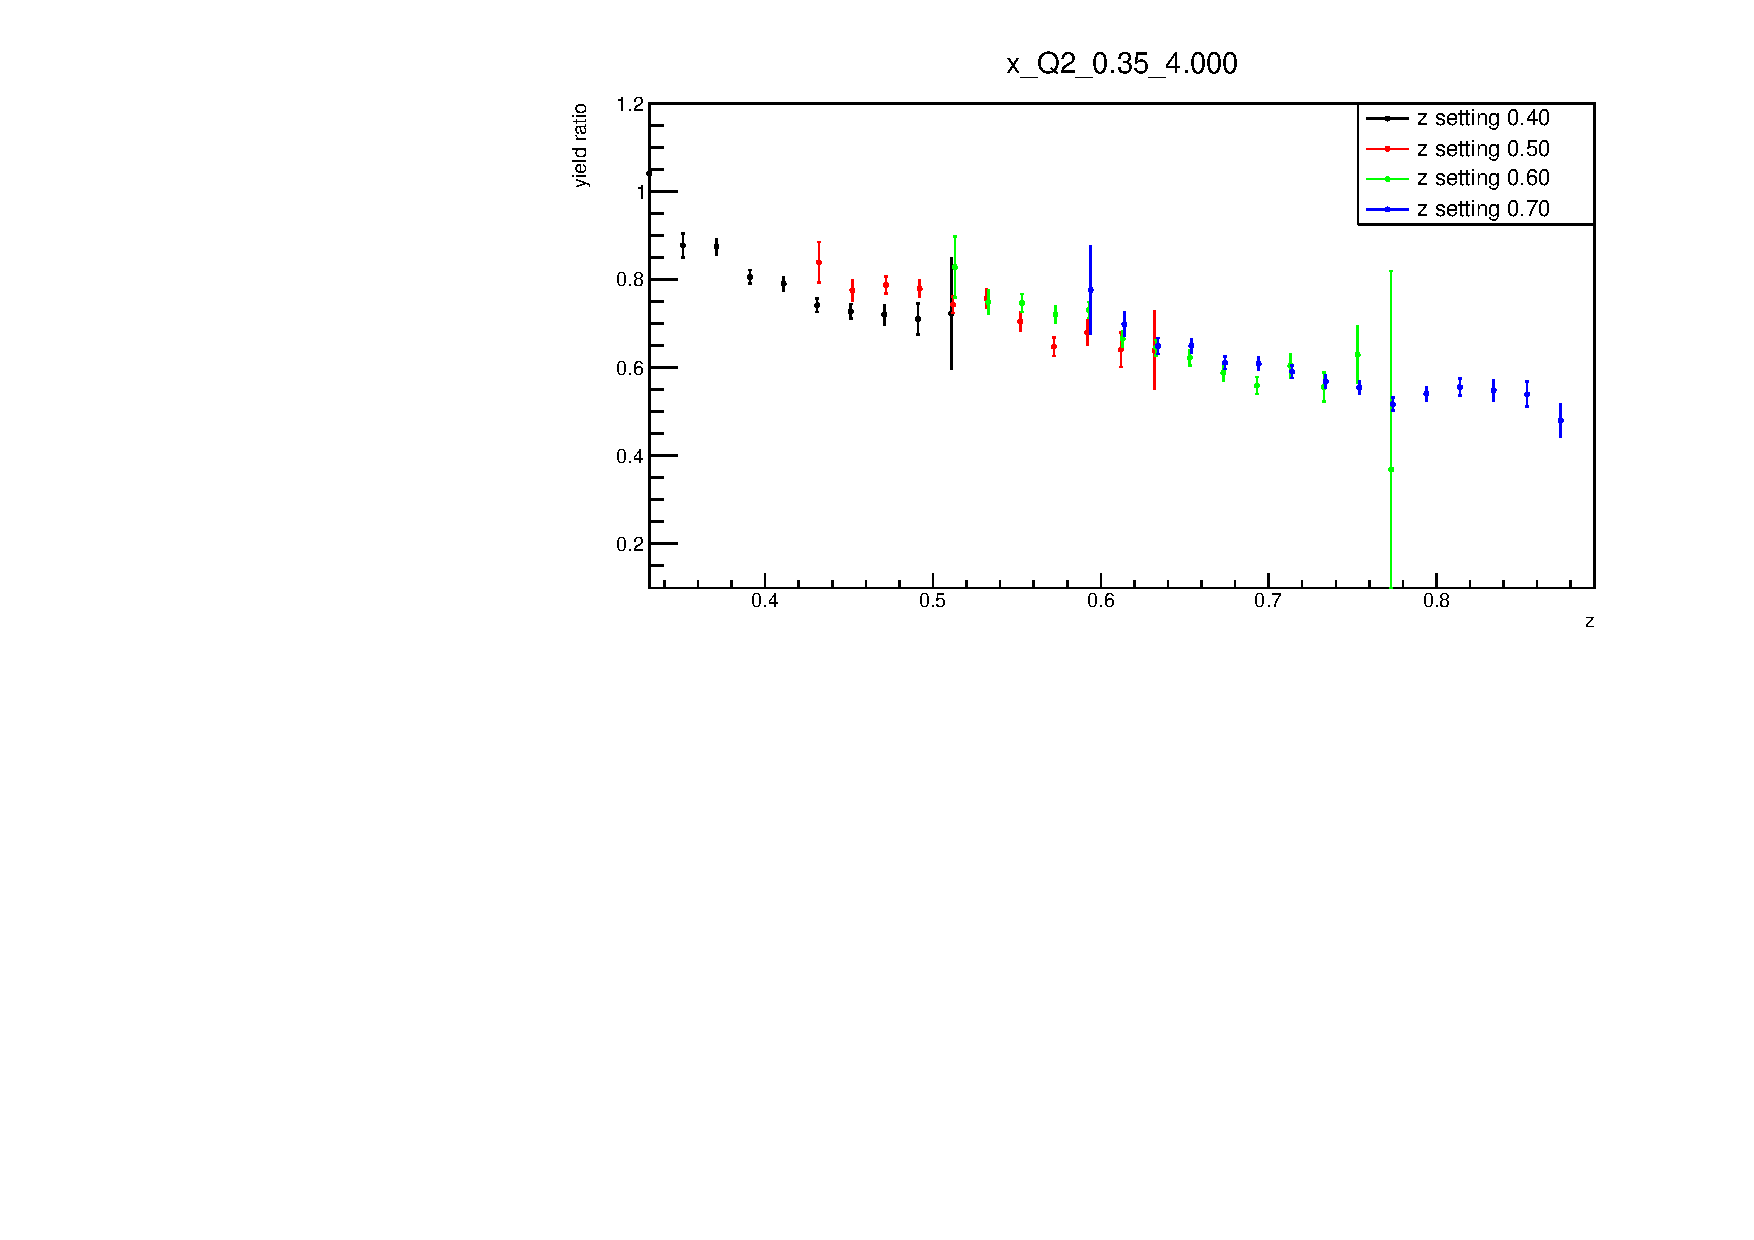
\includegraphics[width = 0.9\textwidth]{results/yield/statistics_corr/x_Q2_0.35_4.000_ratio.pdf}
\end{frame}
\begin{frame}{corrected yield}
\begin{columns}
\begin{column}[T]{0.25\textwidth}
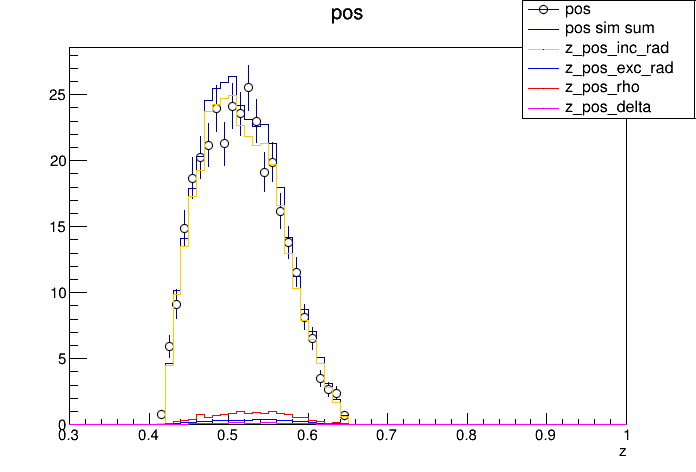
\includegraphics[width = \textwidth]{results/yield/statistics_corr/yield_x_Q2_z_0.40_4.000_0.50_pos.png}
\end{column}
\begin{column}[T]{0.25\textwidth}
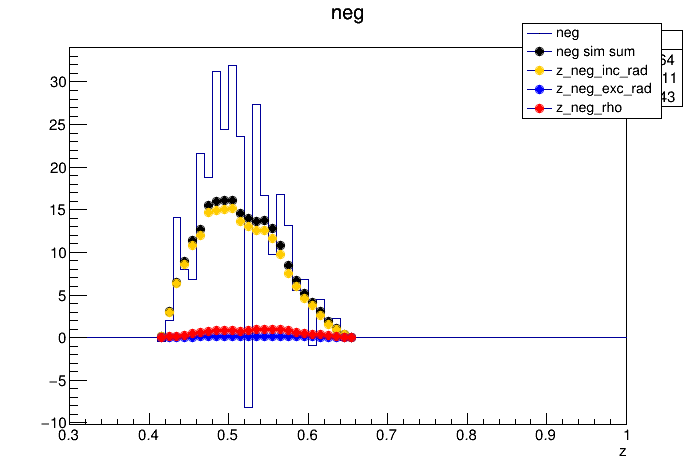
\includegraphics[width = \textwidth]{results/yield/statistics_corr/yield_x_Q2_z_0.40_4.000_0.50_neg.png}
\end{column}
\begin{column}[T]{0.25\textwidth}
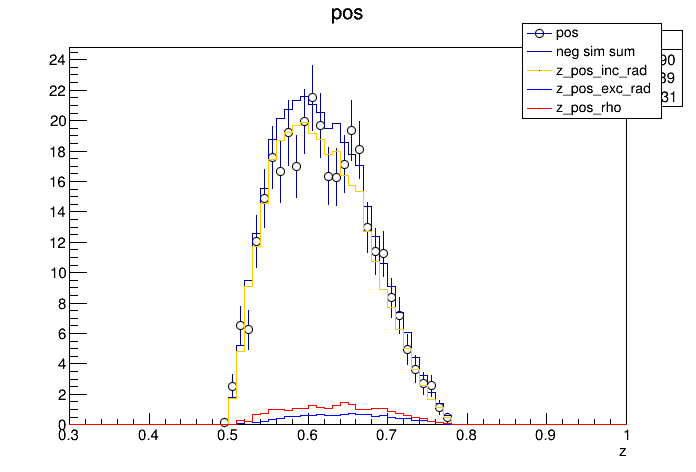
\includegraphics[width = \textwidth]{results/yield/statistics_corr/yield_x_Q2_z_0.40_4.000_0.60_pos.png}
\end{column}
\begin{column}[T]{0.25\textwidth}
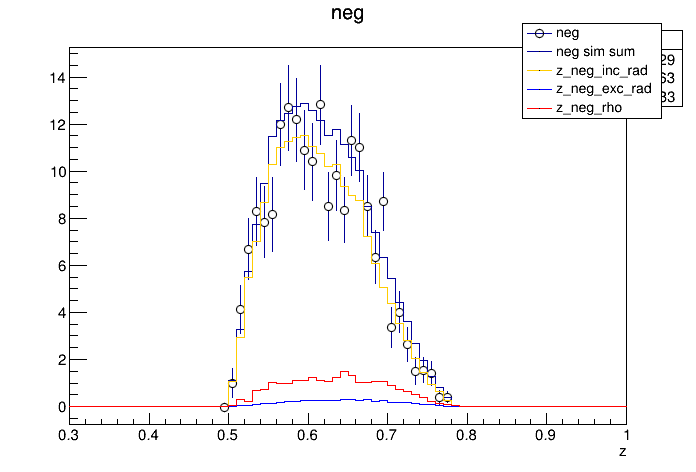
\includegraphics[width = \textwidth]{results/yield/statistics_corr/yield_x_Q2_z_0.40_4.000_0.60_neg.png}
\end{column}
\end{columns}
\begin{columns}
\begin{column}[T]{0.25\textwidth}
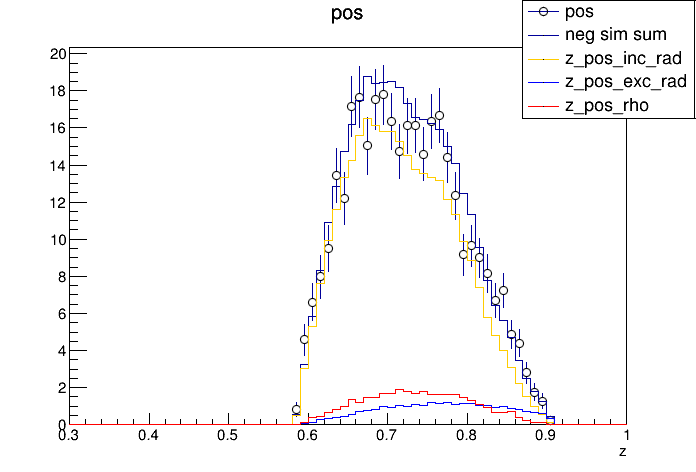
\includegraphics[width = \textwidth]{results/yield/statistics_corr/yield_x_Q2_z_0.40_4.000_0.70_pos.png}
\end{column}
\begin{column}[T]{0.25\textwidth}
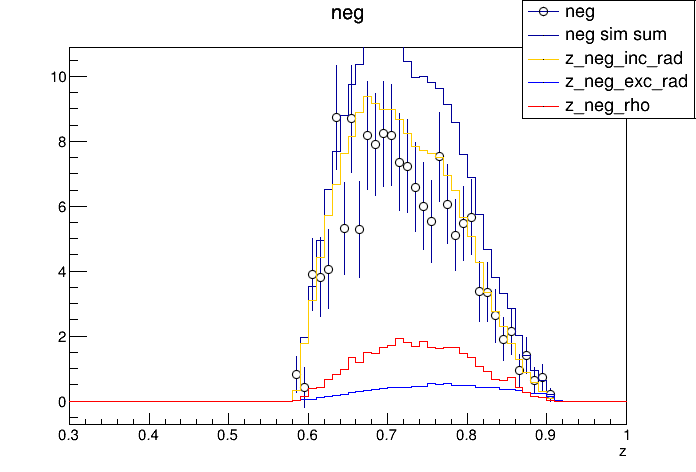
\includegraphics[width = \textwidth]{results/yield/statistics_corr/yield_x_Q2_z_0.40_4.000_0.70_neg.png}
\end{column}
\end{frame}
\begin{frame}{raw yield ratio}
\begin{columns}
\begin{column}[T]{0.5\textwidth}
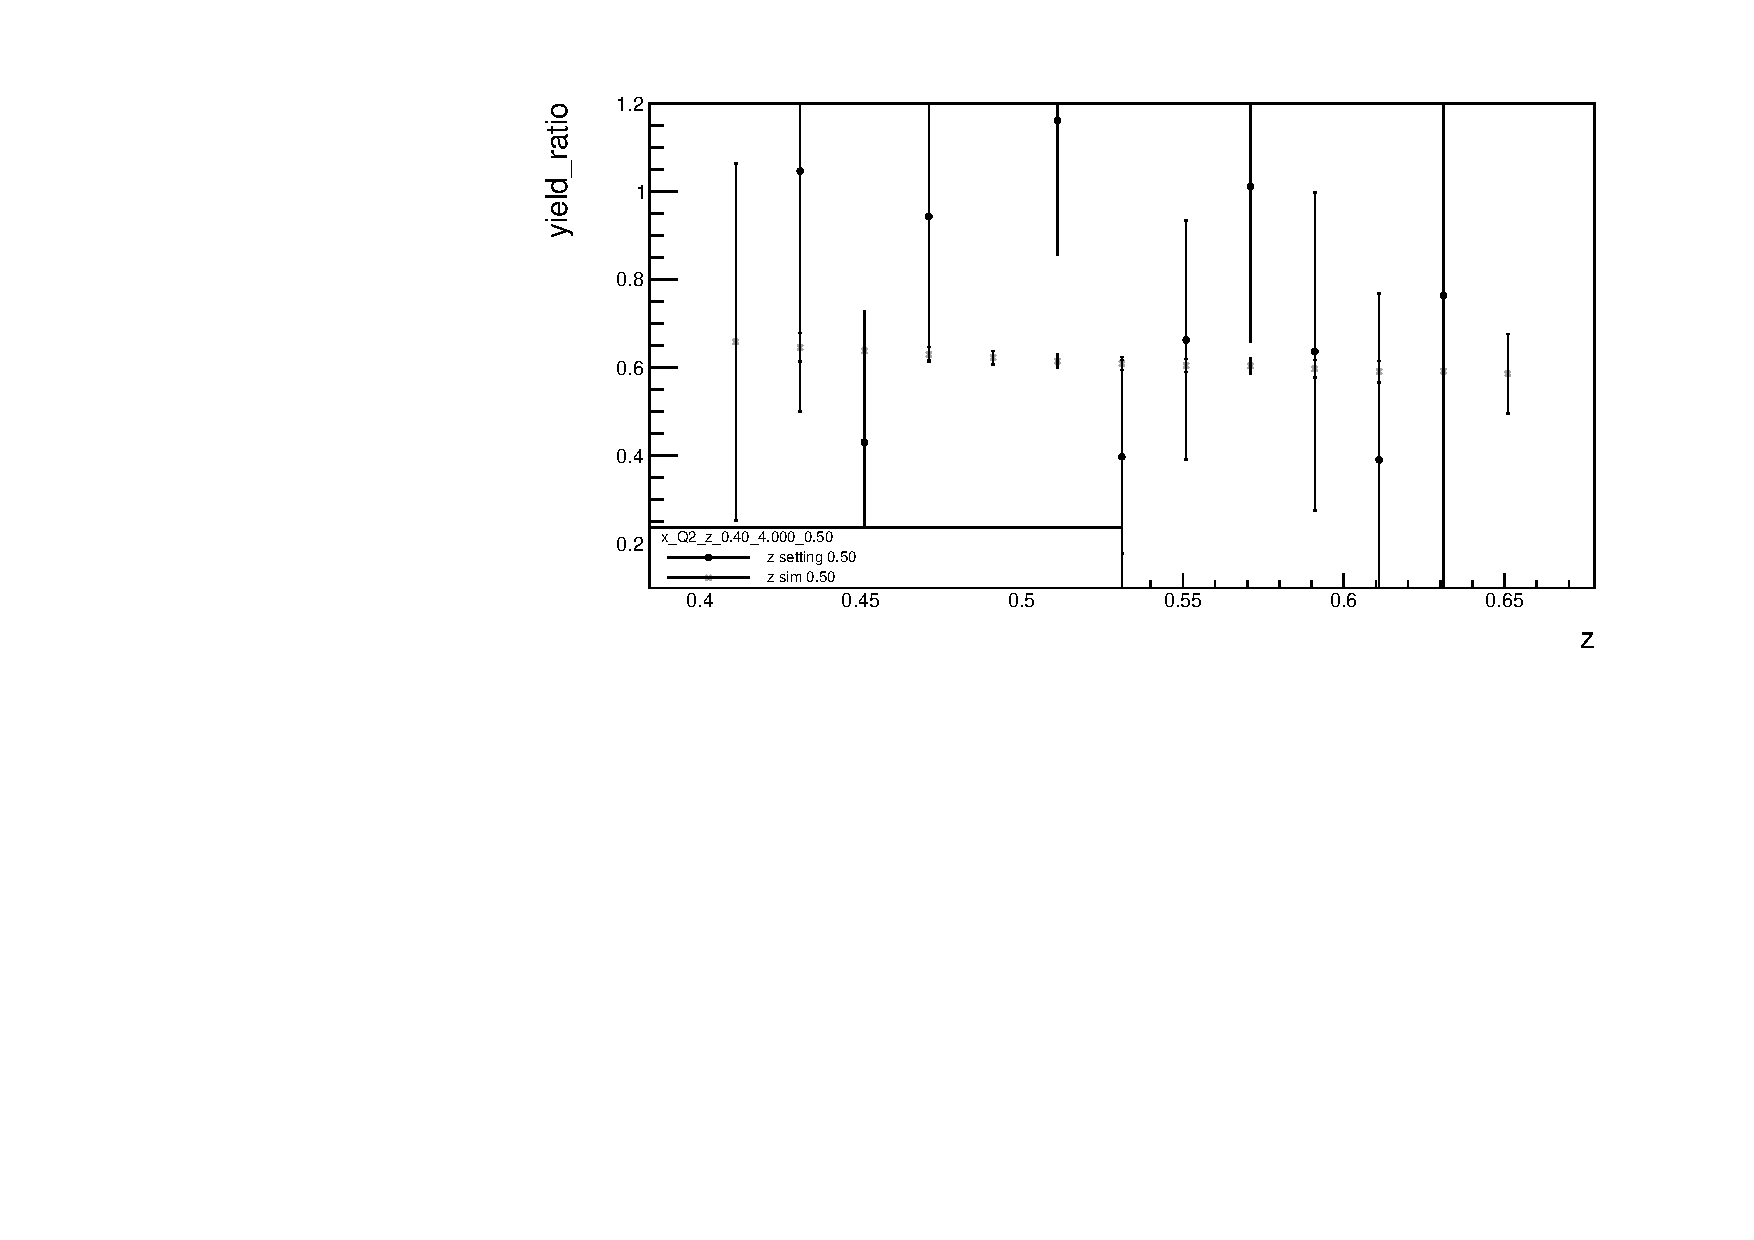
\includegraphics[width = 0.9\textwidth]{results/yield/statistics/x_Q2_z_0.40_4.000_0.50_ratio.pdf}
\end{column}
\begin{column}[T]{0.5\textwidth}
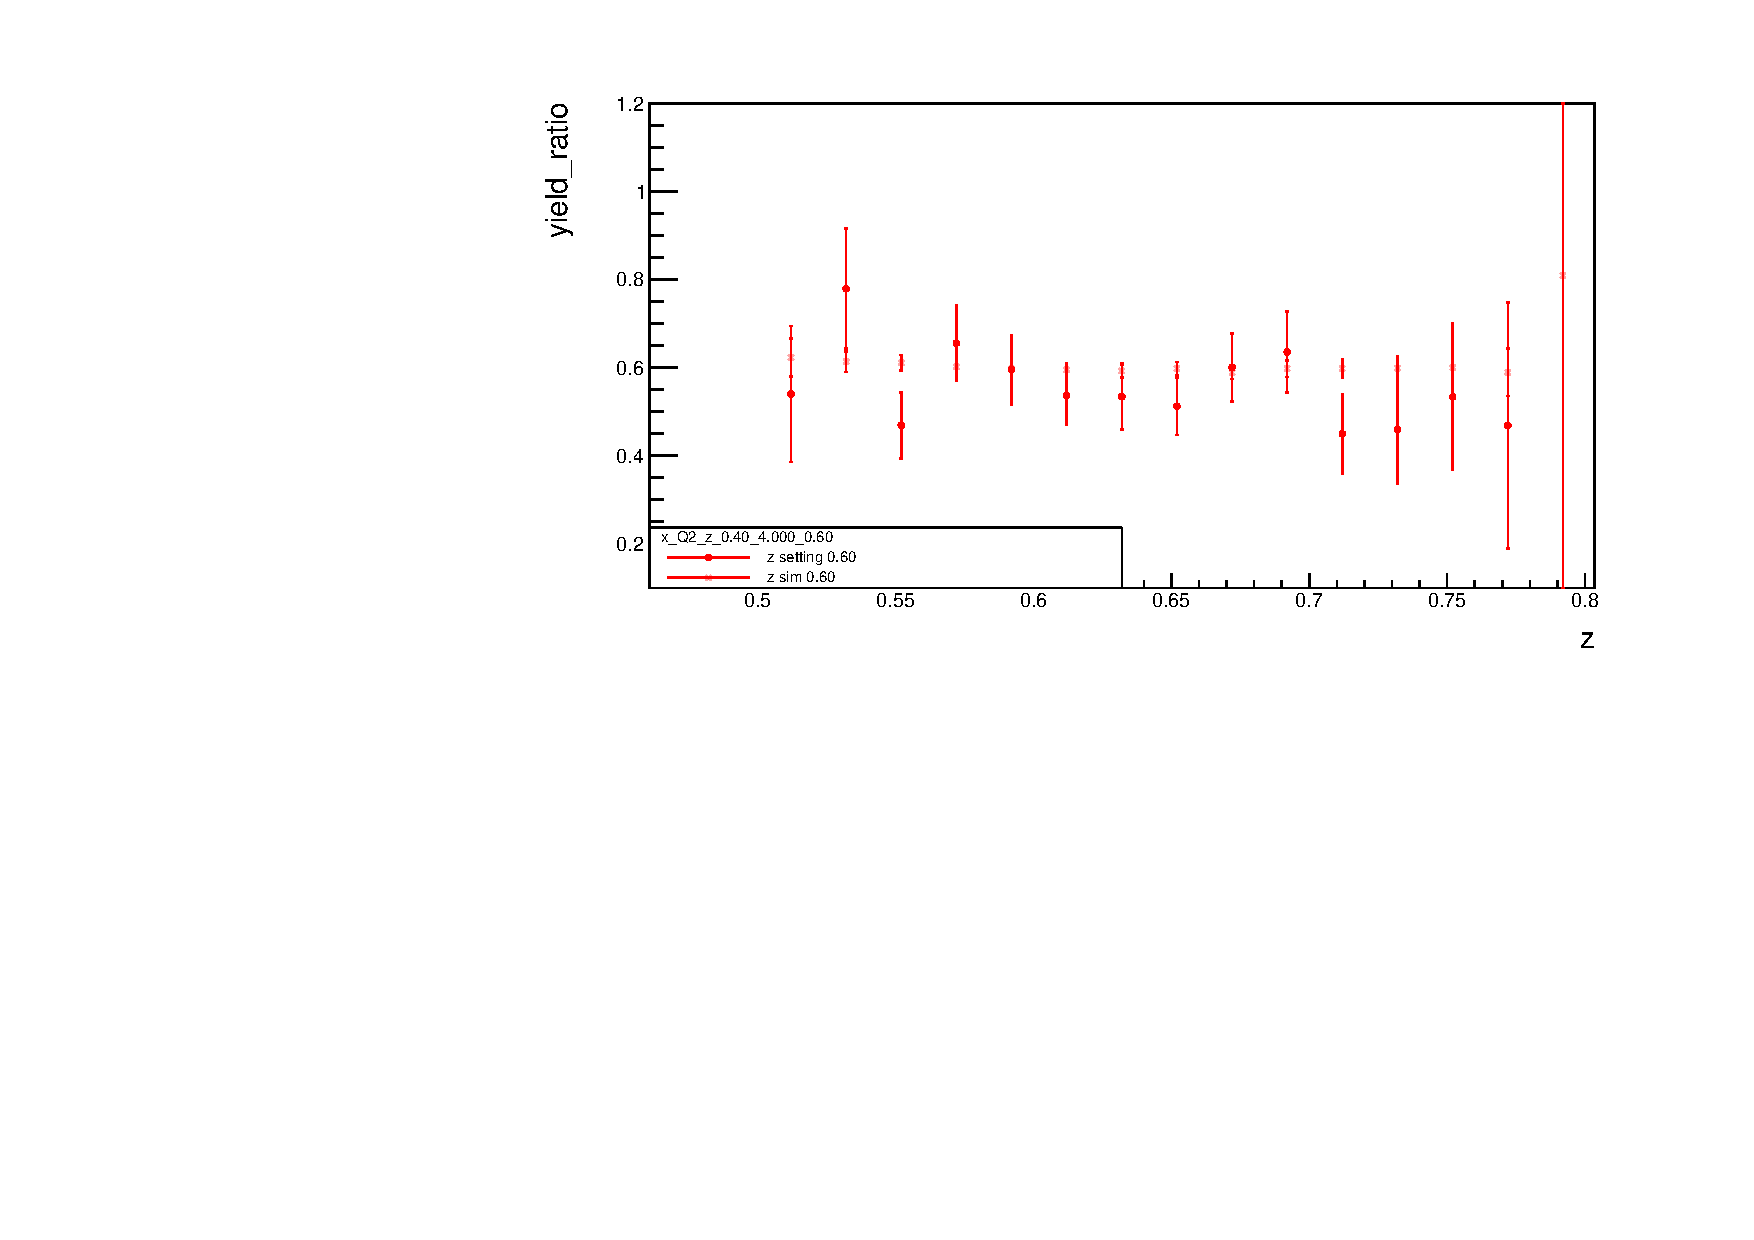
\includegraphics[width = 0.9\textwidth]{results/yield/statistics/x_Q2_z_0.40_4.000_0.60_ratio.pdf}
\end{column}
\end{columns}
\begin{columns}
\begin{column}[T]{0.5\textwidth}
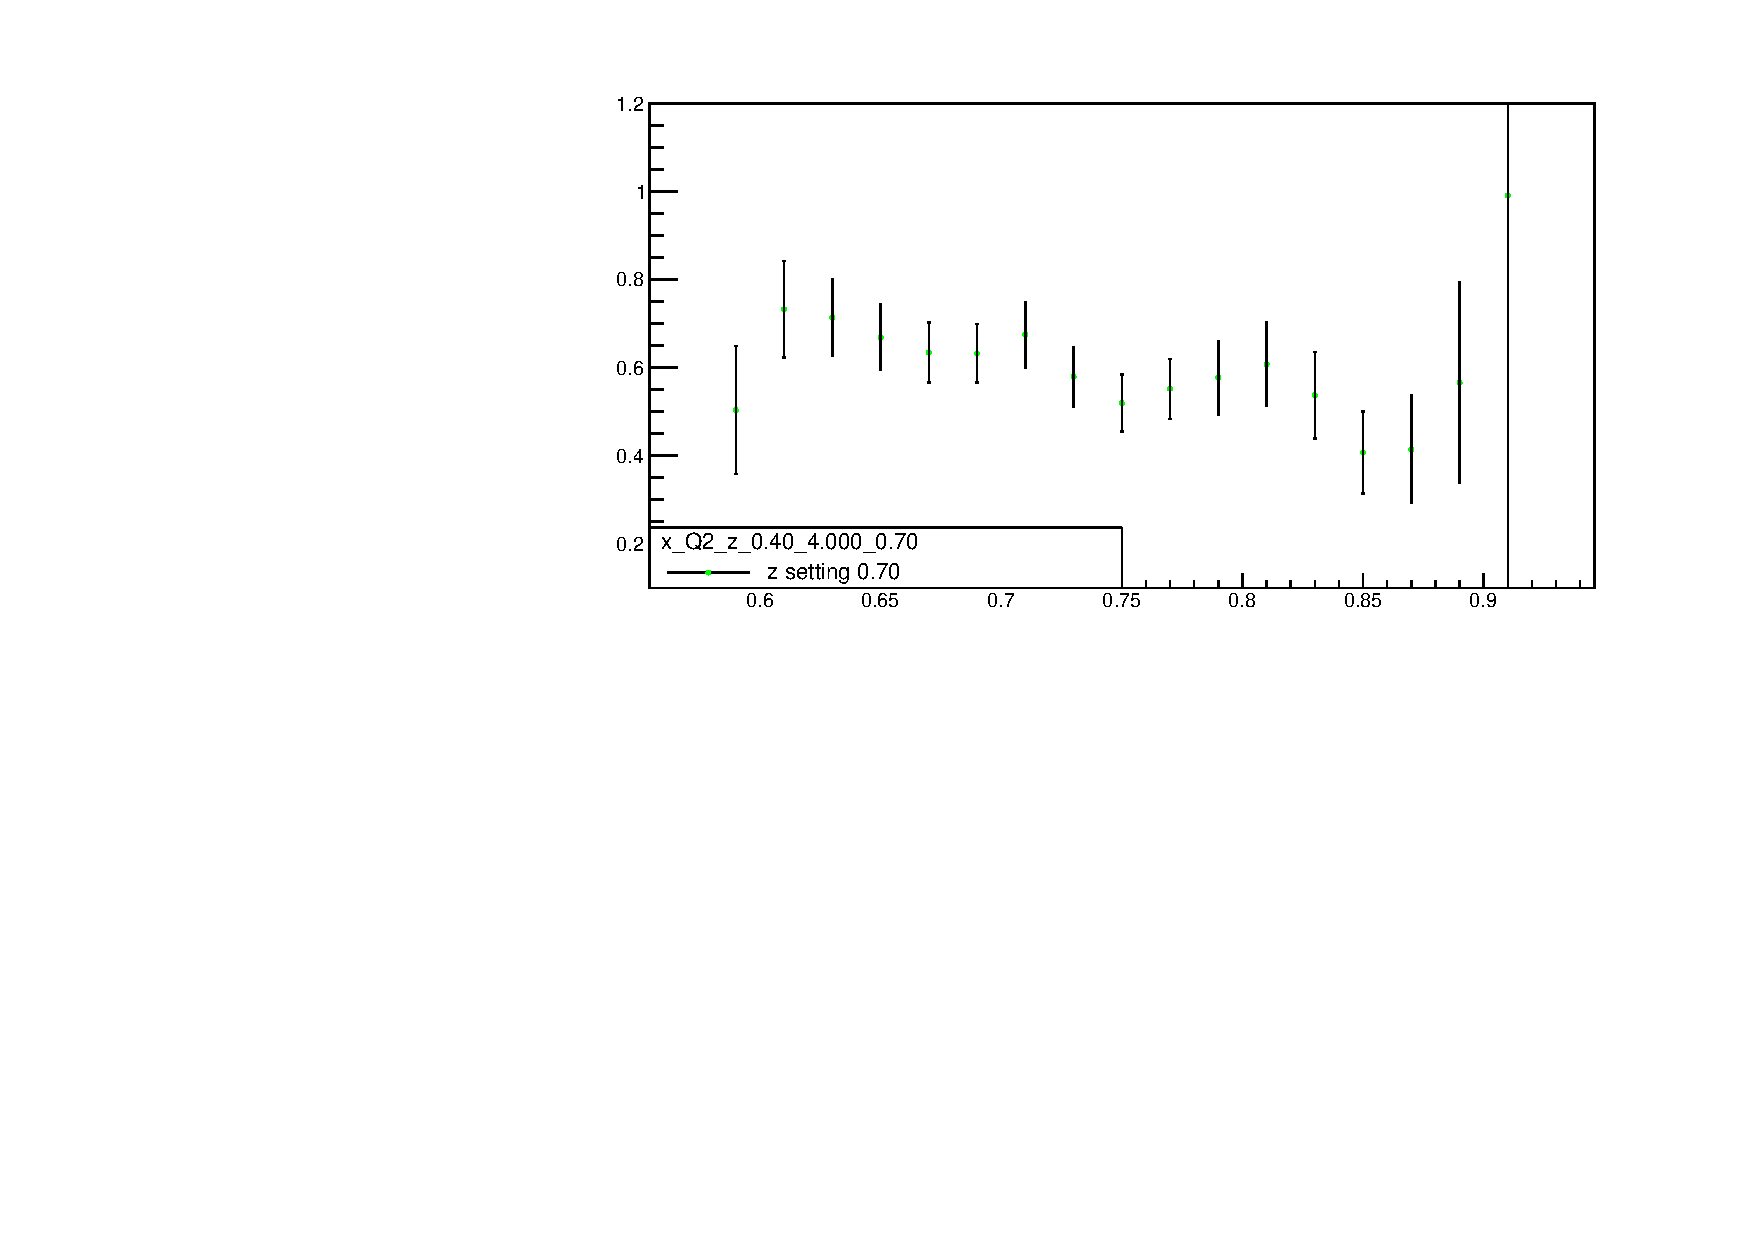
\includegraphics[width = 0.9\textwidth]{results/yield/statistics/x_Q2_z_0.40_4.000_0.70_ratio.pdf}
\end{column}
\begin{column}[T]{0.5\textwidth}
\end{column}
\end{columns}
\end{frame}
\begin{frame}{TE,pi eff, pi purity corrected yield ratio}
\begin{columns}
\begin{column}[T]{0.5\textwidth}
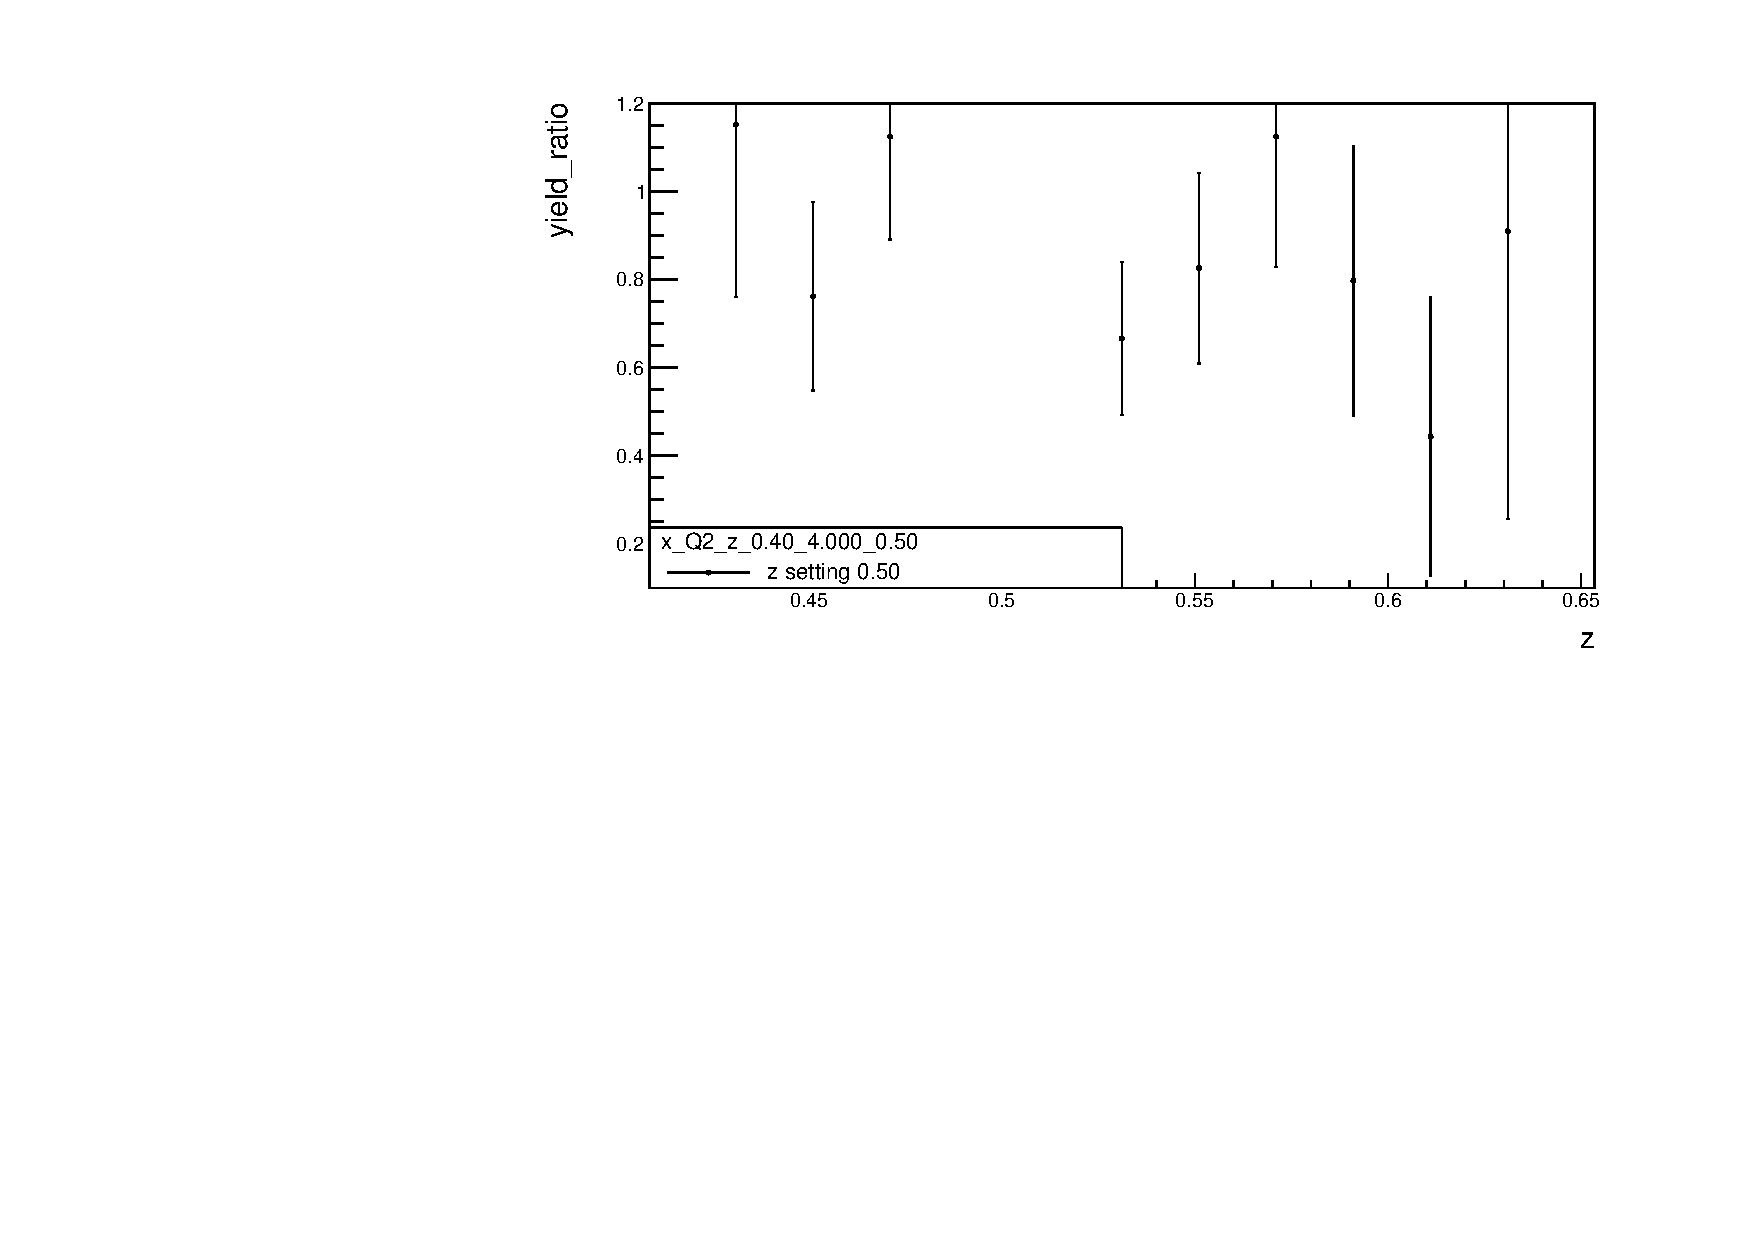
\includegraphics[width = 0.9\textwidth]{results/yield/statistics_corr/x_Q2_z_0.40_4.000_0.50_ratio.pdf}
\end{column}
\begin{column}[T]{0.5\textwidth}
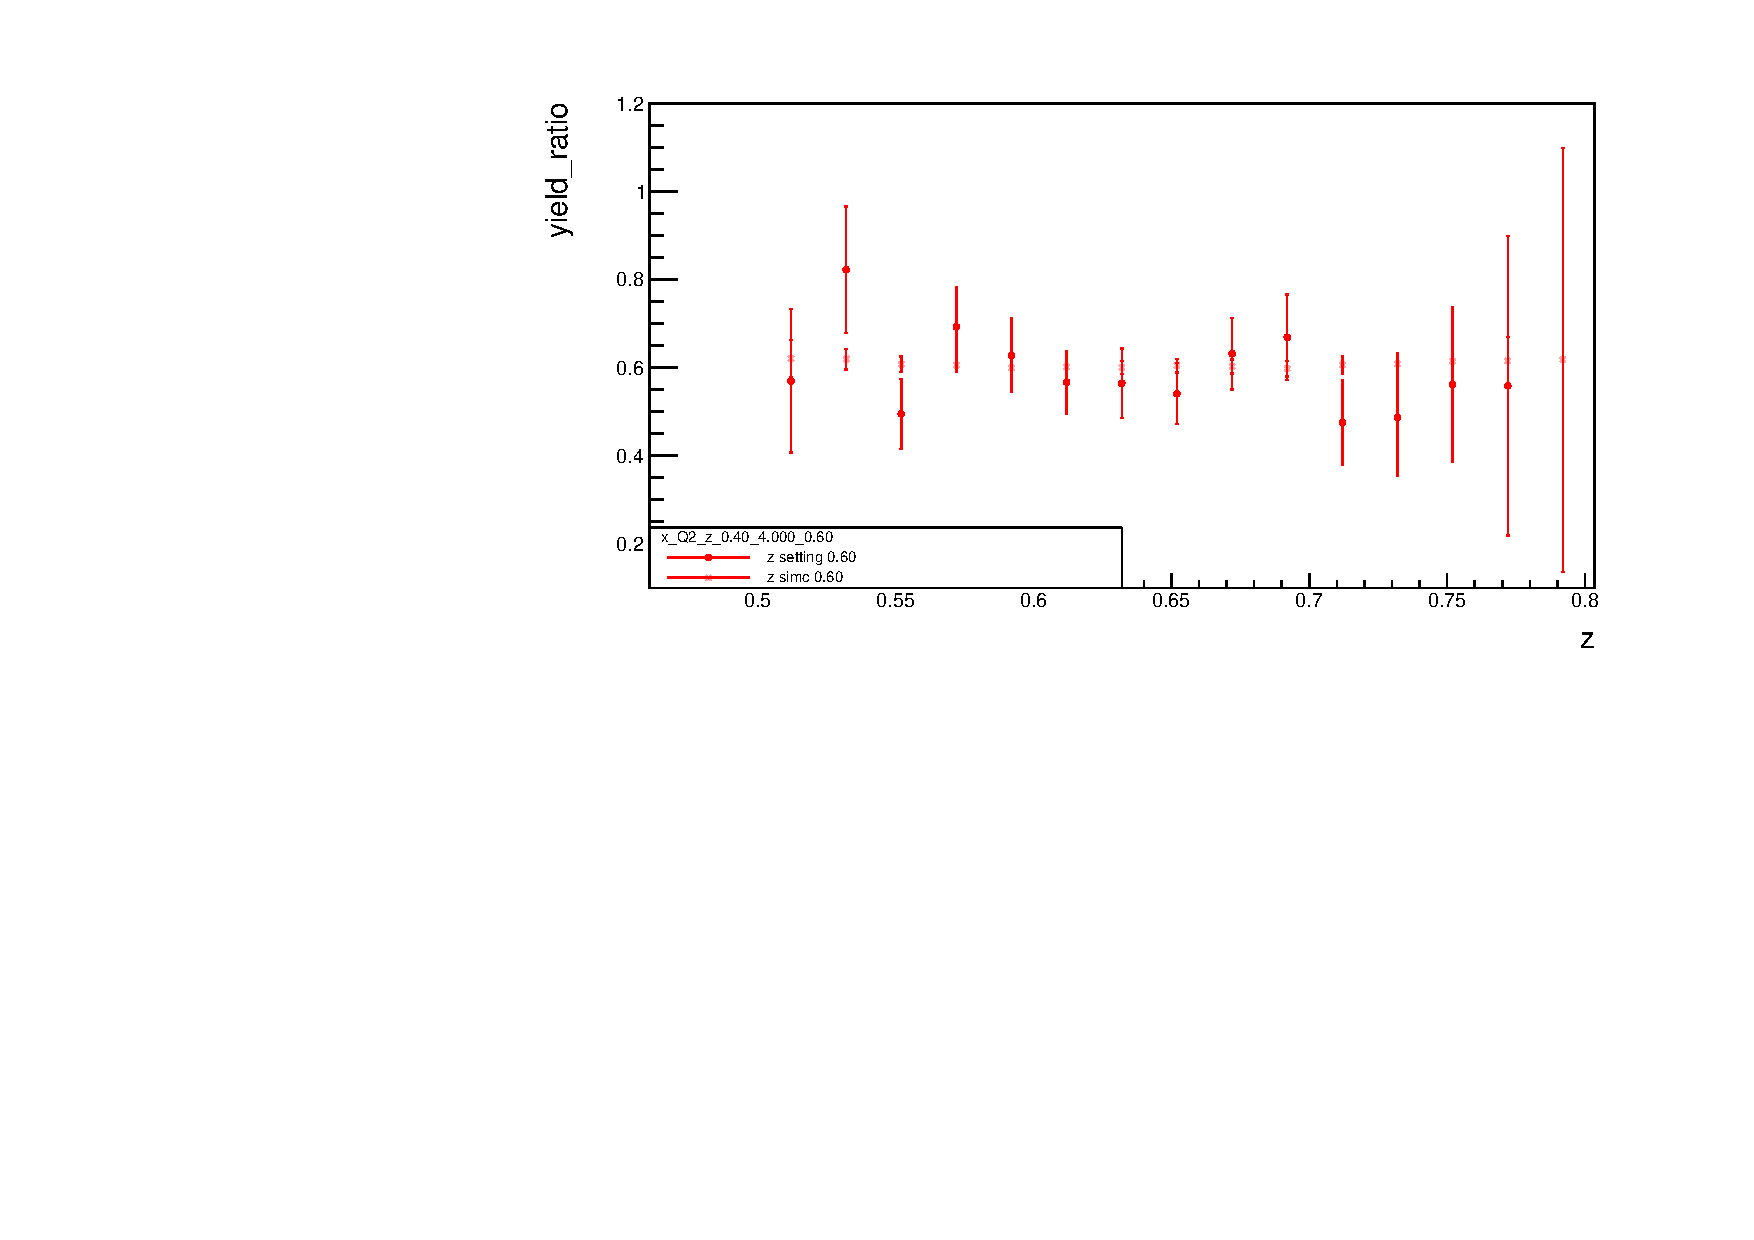
\includegraphics[width = 0.9\textwidth]{results/yield/statistics_corr/x_Q2_z_0.40_4.000_0.60_ratio.pdf}
\end{column}
\end{columns}
\begin{columns}
\begin{column}[T]{0.5\textwidth}
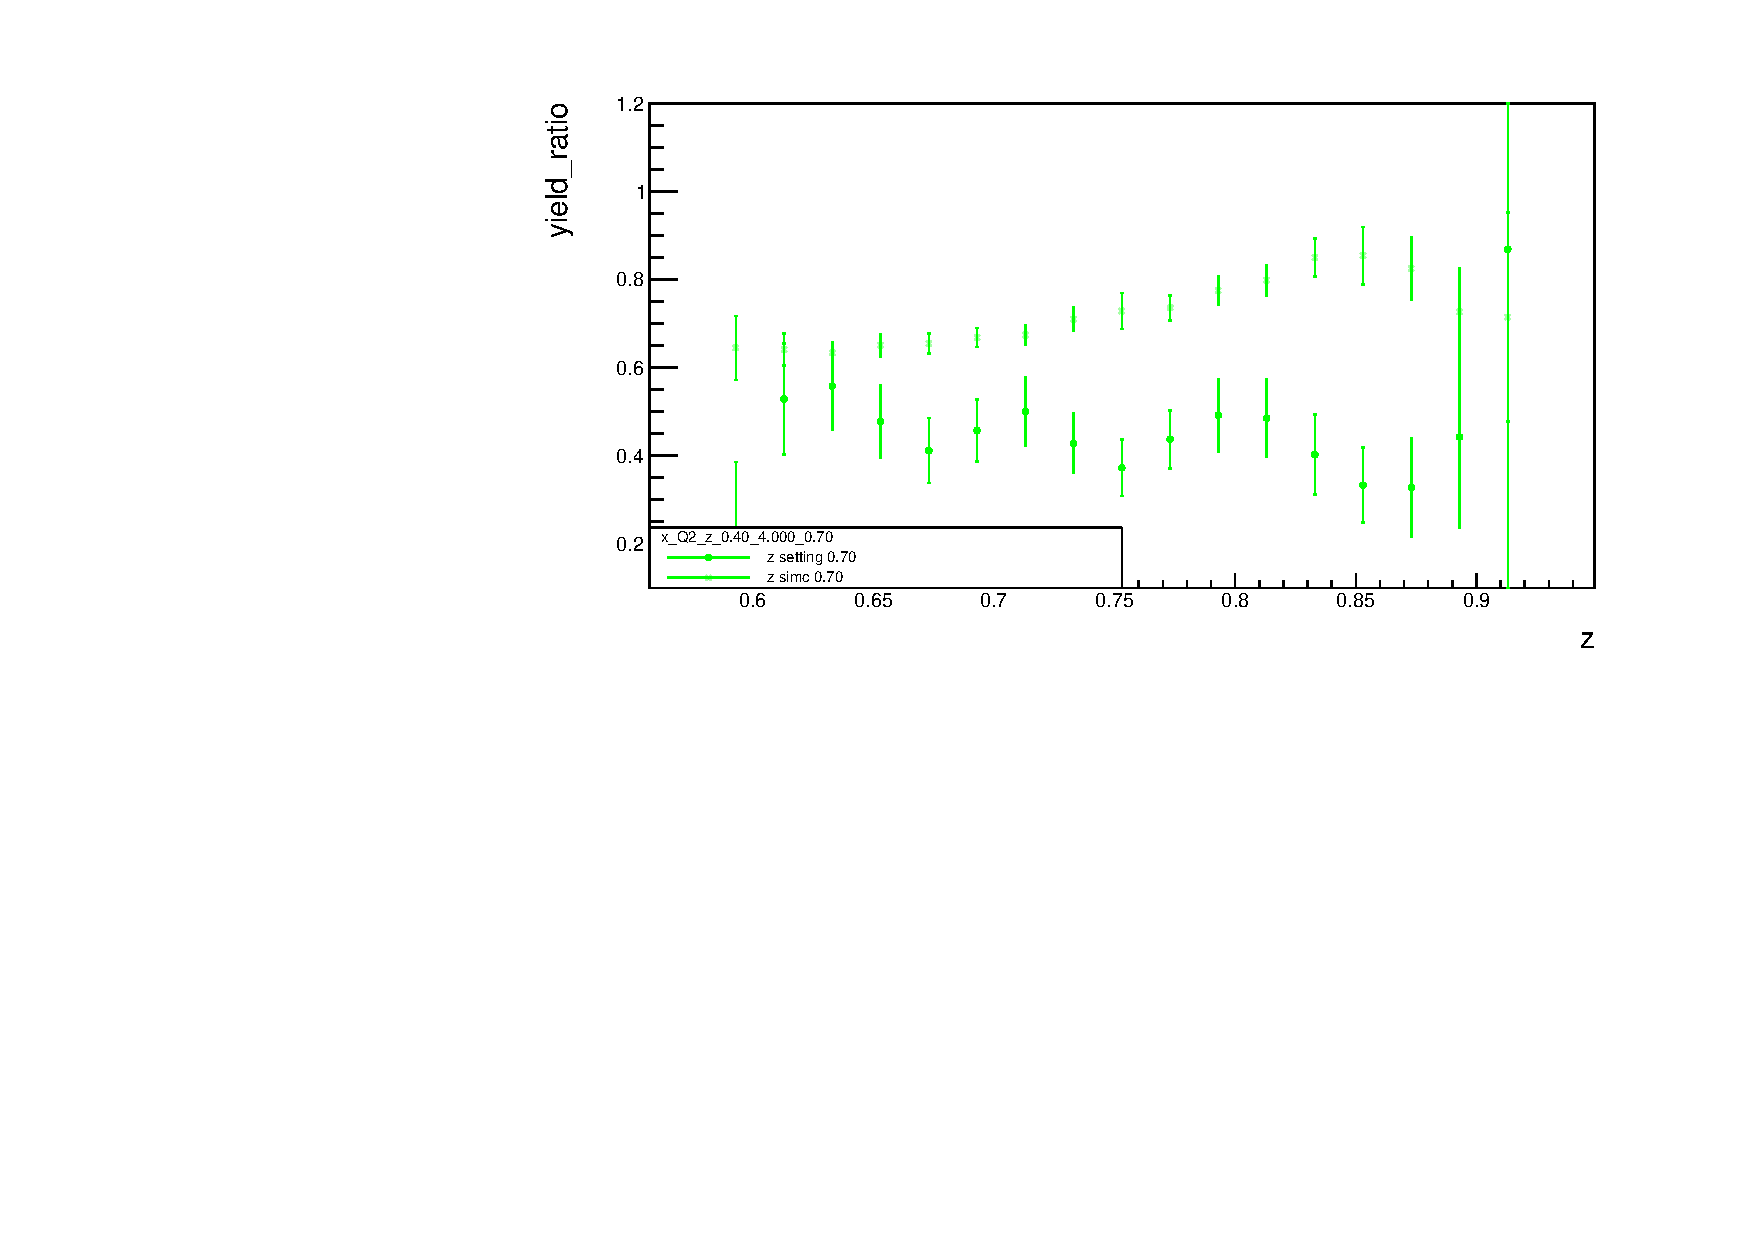
\includegraphics[width = 0.9\textwidth]{results/yield/statistics_corr/x_Q2_z_0.40_4.000_0.70_ratio.pdf}
\end{column}
\begin{column}[T]{0.5\textwidth}
\end{column}
\end{columns}
\end{frame}
\begin{frame}{raw yield ratio}
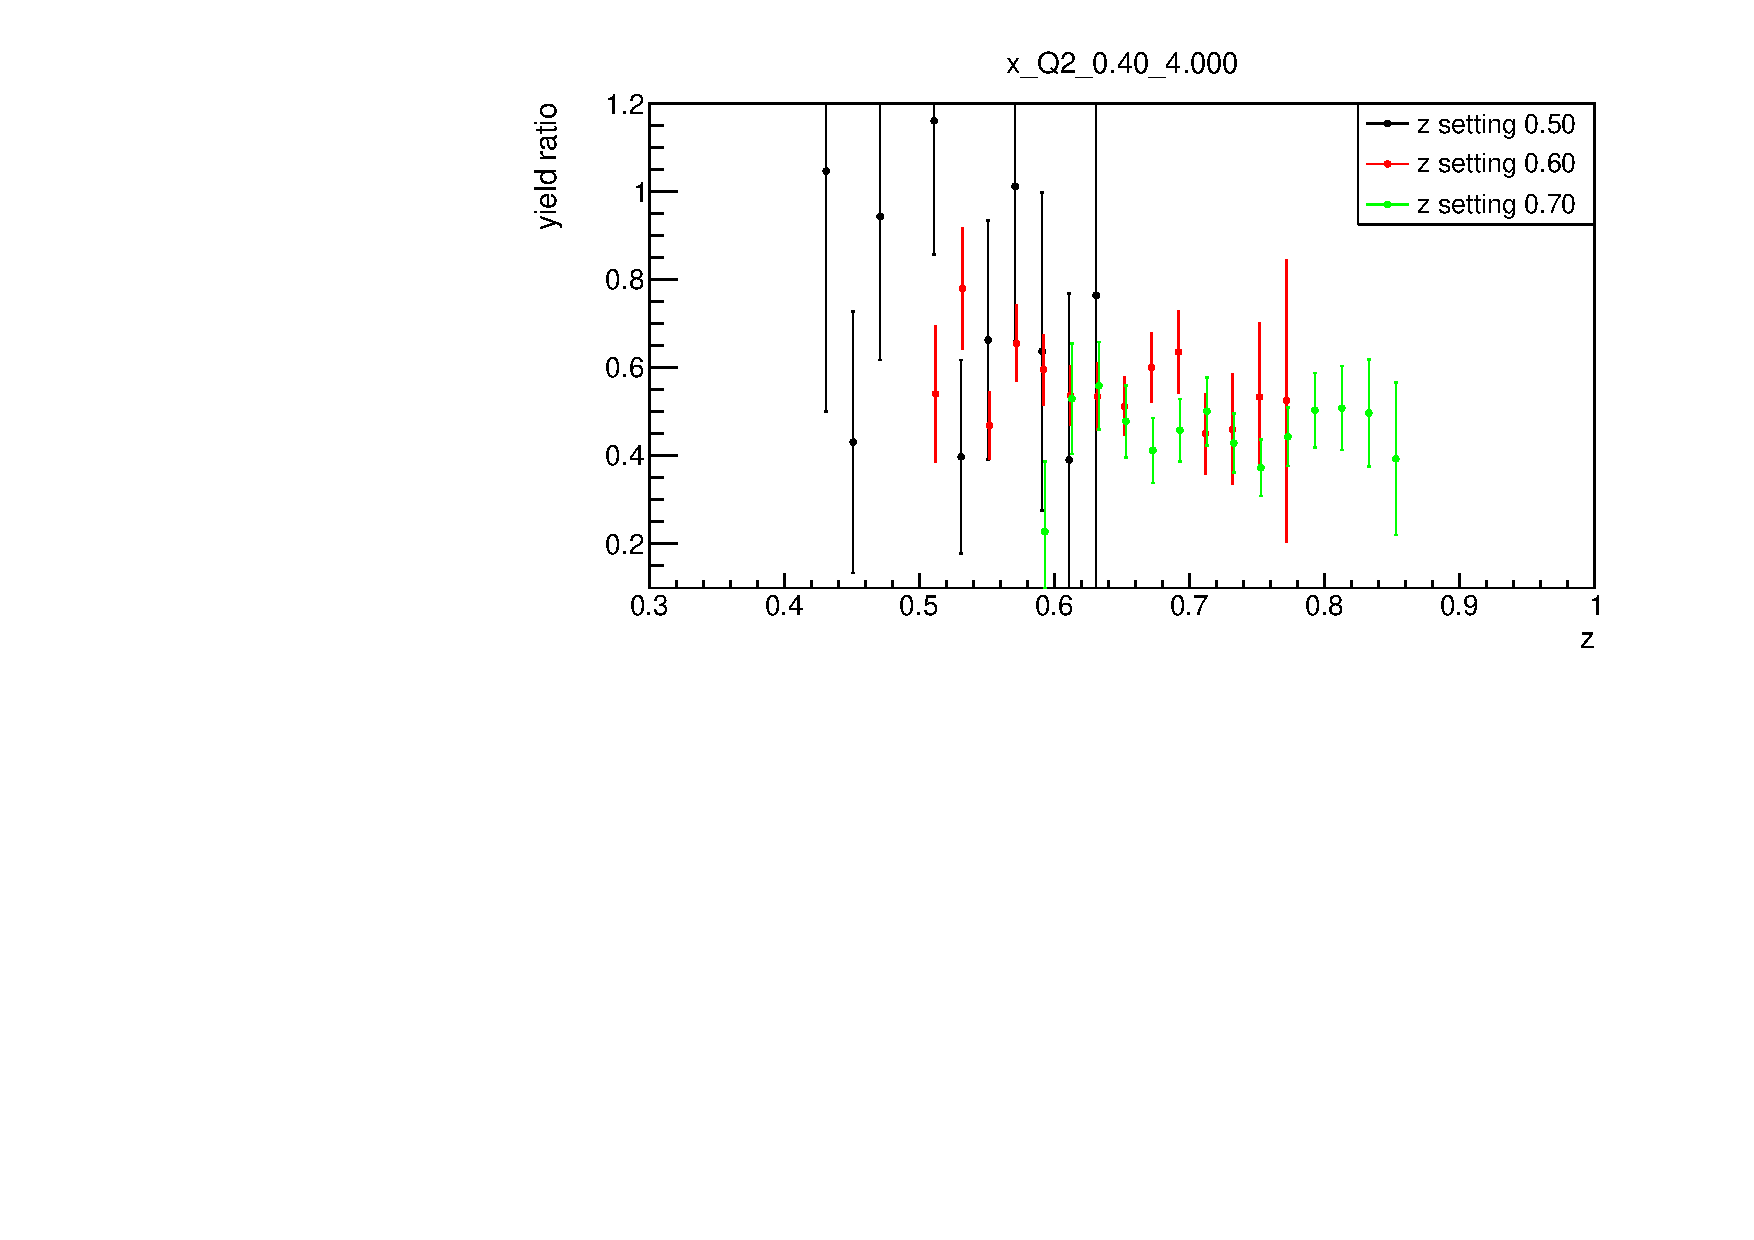
\includegraphics[width = 0.9\textwidth]{results/yield/statistics/x_Q2_0.40_4.000_ratio.pdf}
\end{frame}
\begin{frame}{TE,pi eff, pi purity corrected yield ratio}
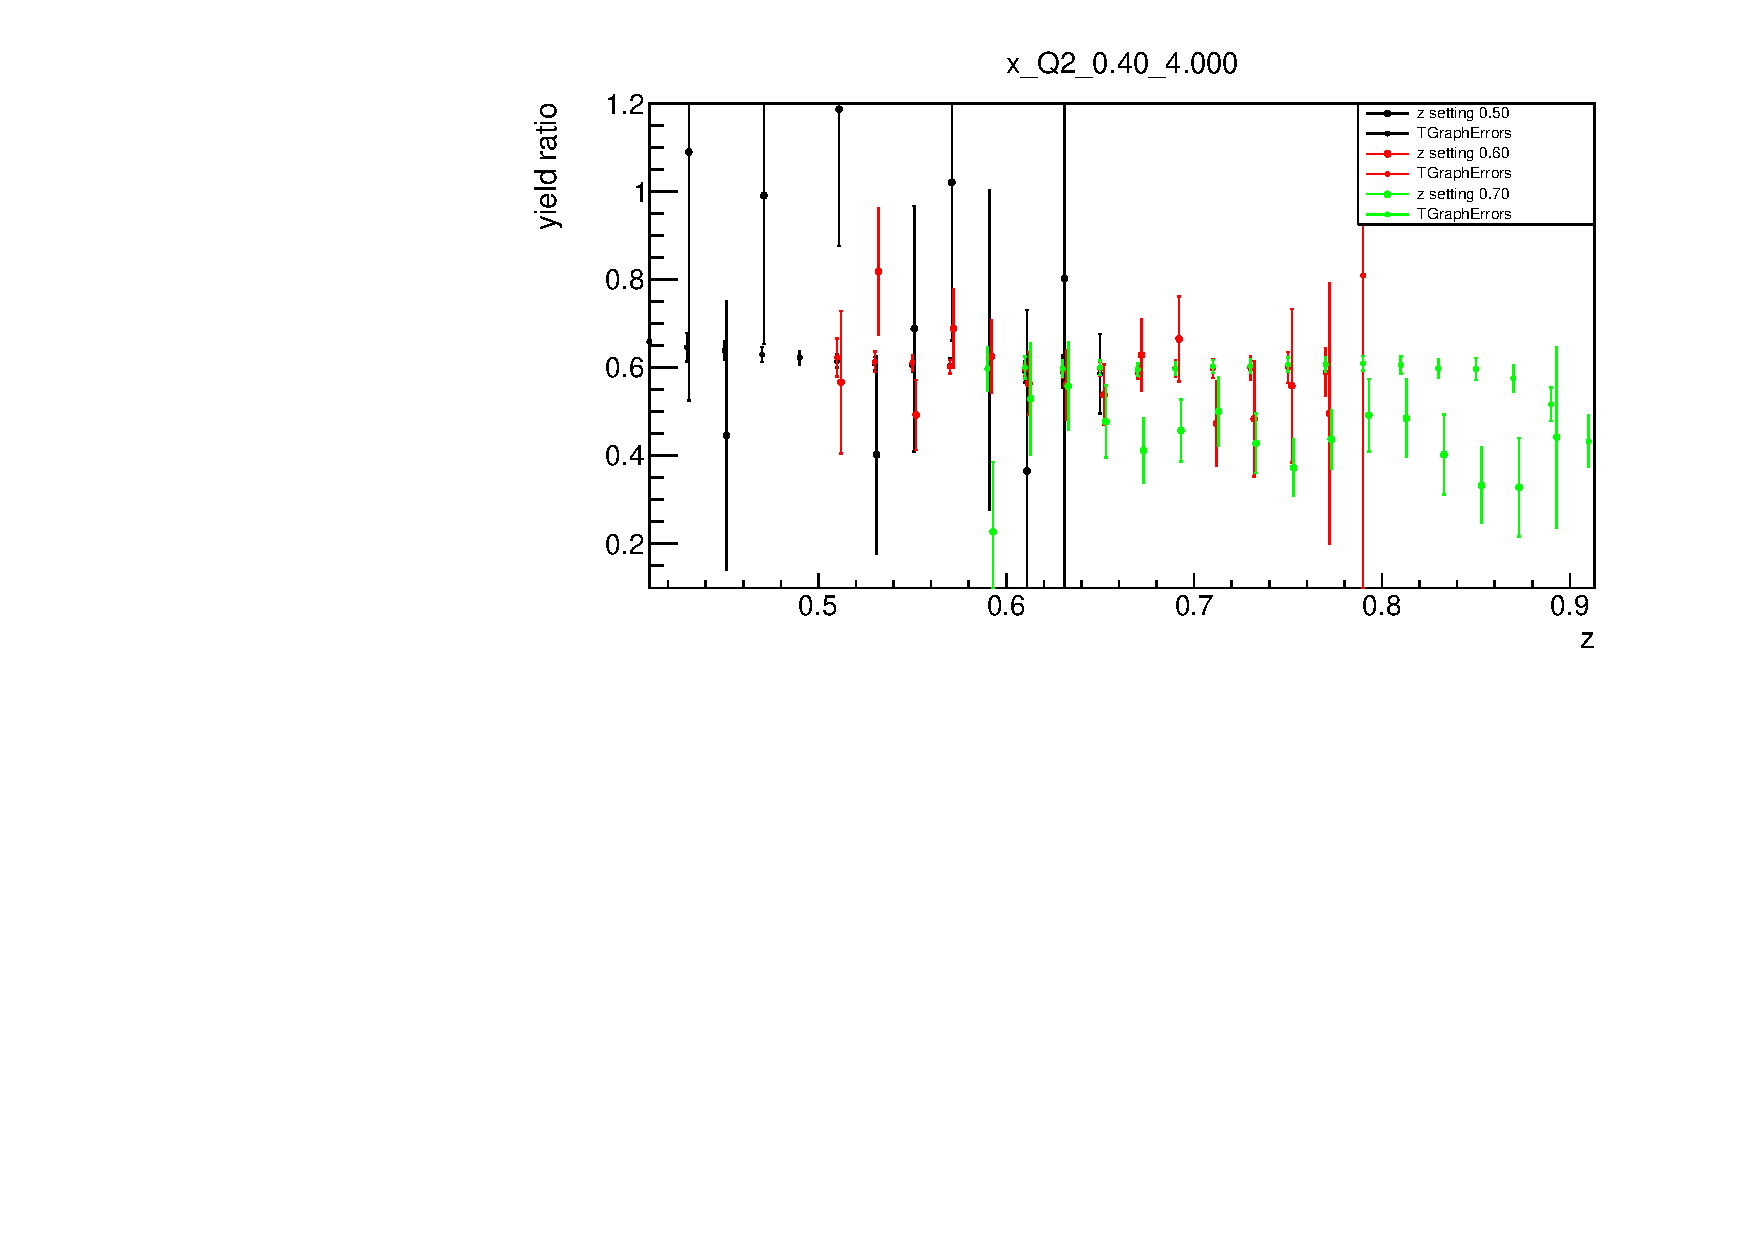
\includegraphics[width = 0.9\textwidth]{results/yield/statistics_corr/x_Q2_0.40_4.000_ratio.pdf}
\end{frame}
\begin{frame}{corrected yield}
\begin{columns}
\begin{column}[T]{0.25\textwidth}
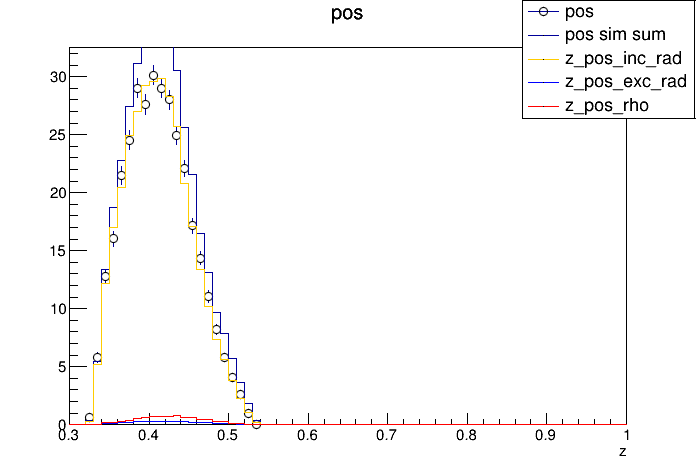
\includegraphics[width = \textwidth]{results/yield/statistics_corr/yield_x_Q2_z_0.45_3.898_0.40_pos.png}
\end{column}
\begin{column}[T]{0.25\textwidth}
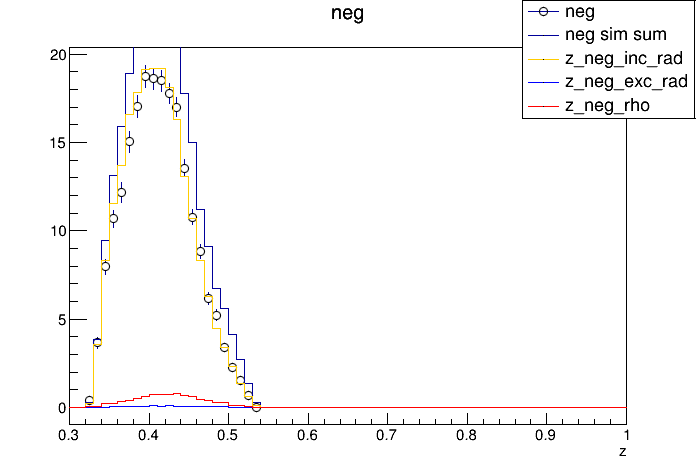
\includegraphics[width = \textwidth]{results/yield/statistics_corr/yield_x_Q2_z_0.45_3.898_0.40_neg.png}
\end{column}
\begin{column}[T]{0.25\textwidth}
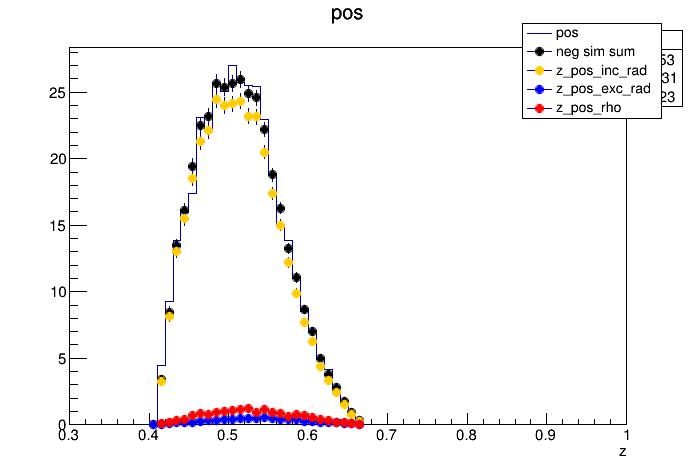
\includegraphics[width = \textwidth]{results/yield/statistics_corr/yield_x_Q2_z_0.45_3.898_0.50_pos.png}
\end{column}
\begin{column}[T]{0.25\textwidth}
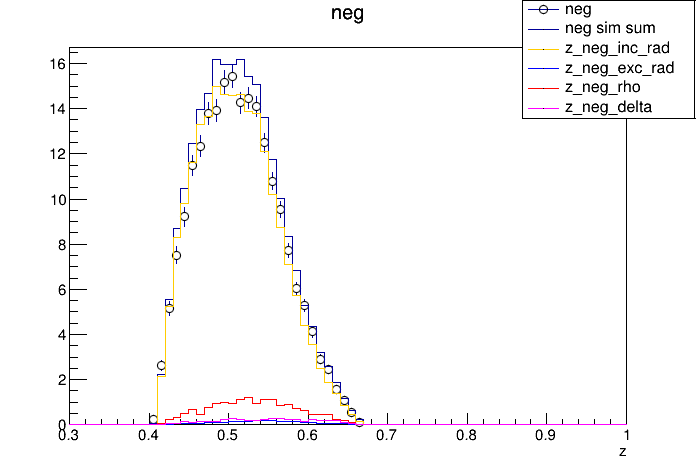
\includegraphics[width = \textwidth]{results/yield/statistics_corr/yield_x_Q2_z_0.45_3.898_0.50_neg.png}
\end{column}
\end{columns}
\begin{columns}
\begin{column}[T]{0.25\textwidth}
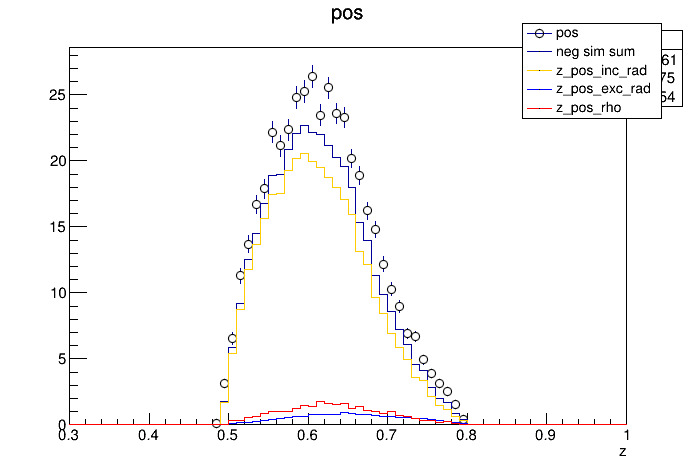
\includegraphics[width = \textwidth]{results/yield/statistics_corr/yield_x_Q2_z_0.45_3.898_0.60_pos.png}
\end{column}
\begin{column}[T]{0.25\textwidth}
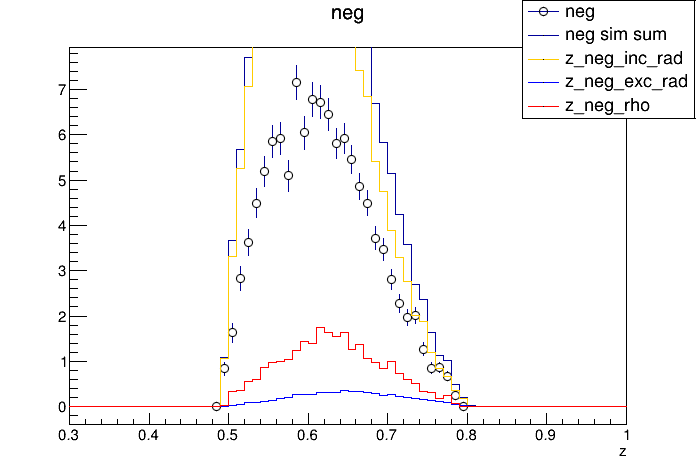
\includegraphics[width = \textwidth]{results/yield/statistics_corr/yield_x_Q2_z_0.45_3.898_0.60_neg.png}
\end{column}
\begin{column}[T]{0.25\textwidth}
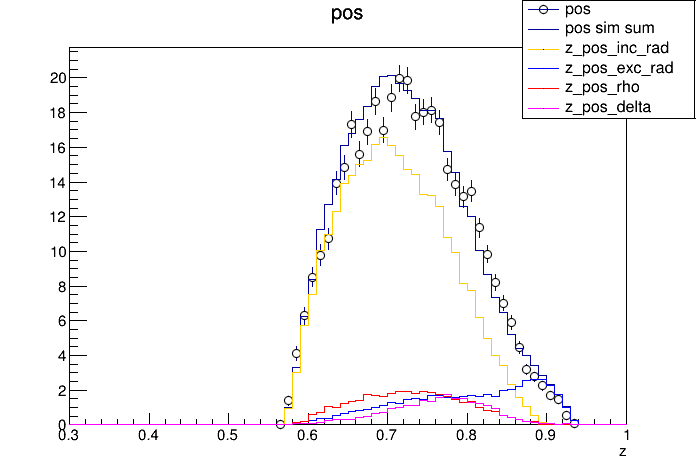
\includegraphics[width = \textwidth]{results/yield/statistics_corr/yield_x_Q2_z_0.45_3.898_0.70_pos.png}
\end{column}
\begin{column}[T]{0.25\textwidth}
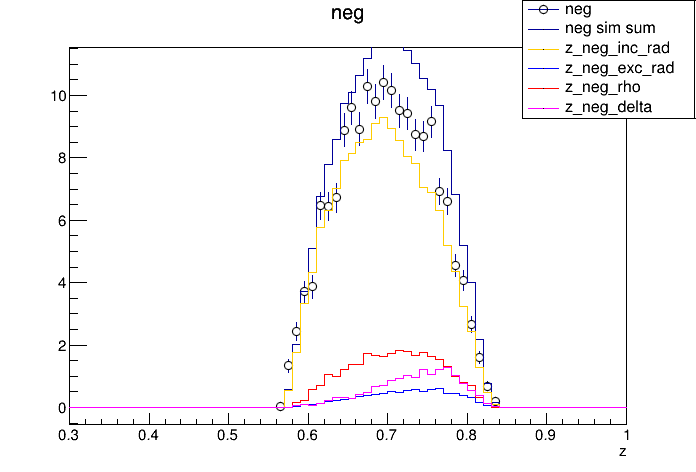
\includegraphics[width = \textwidth]{results/yield/statistics_corr/yield_x_Q2_z_0.45_3.898_0.70_neg.png}
\end{column}
\end{columns}
\end{frame}
\begin{frame}{raw yield ratio}
\begin{columns}
\begin{column}[T]{0.5\textwidth}
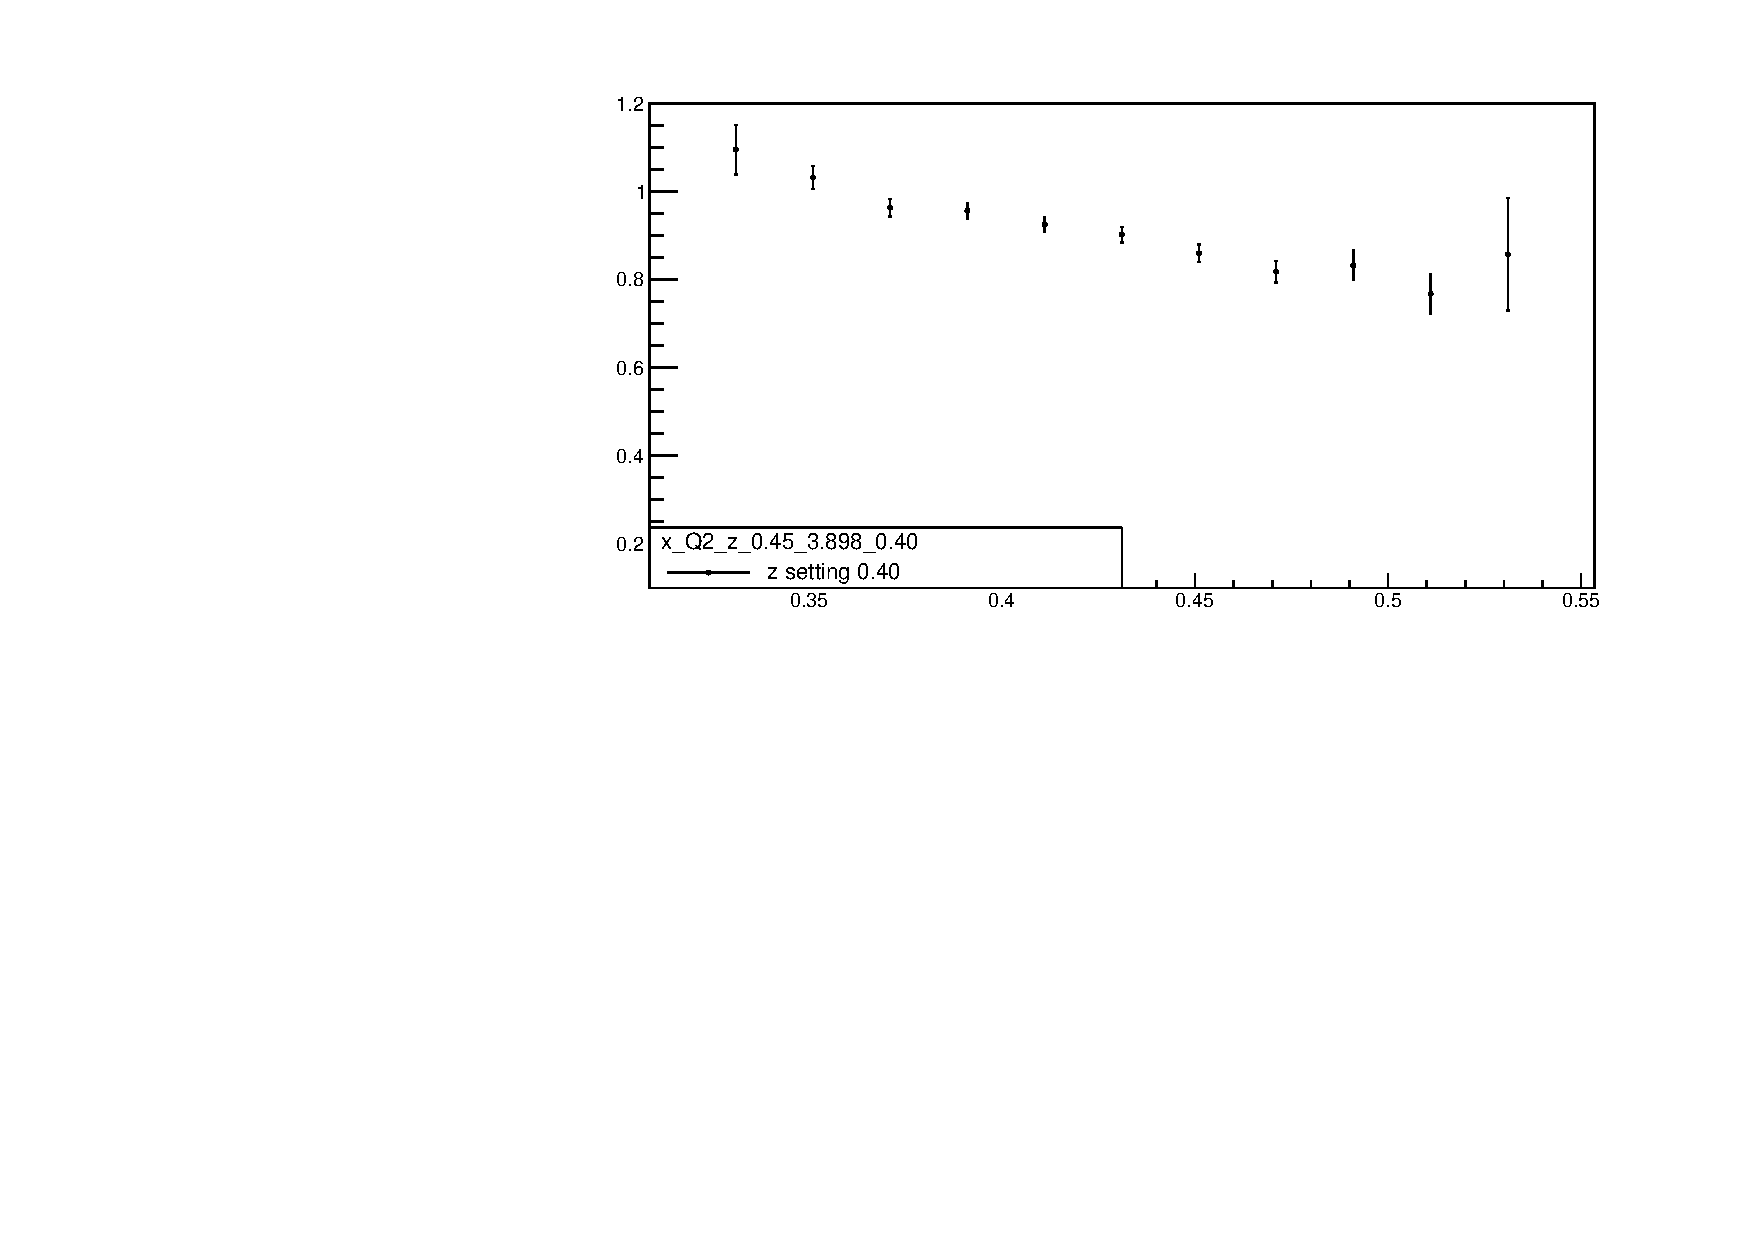
\includegraphics[width = 0.9\textwidth]{results/yield/statistics/x_Q2_z_0.45_3.898_0.40_ratio.pdf}
\end{column}
\begin{column}[T]{0.5\textwidth}
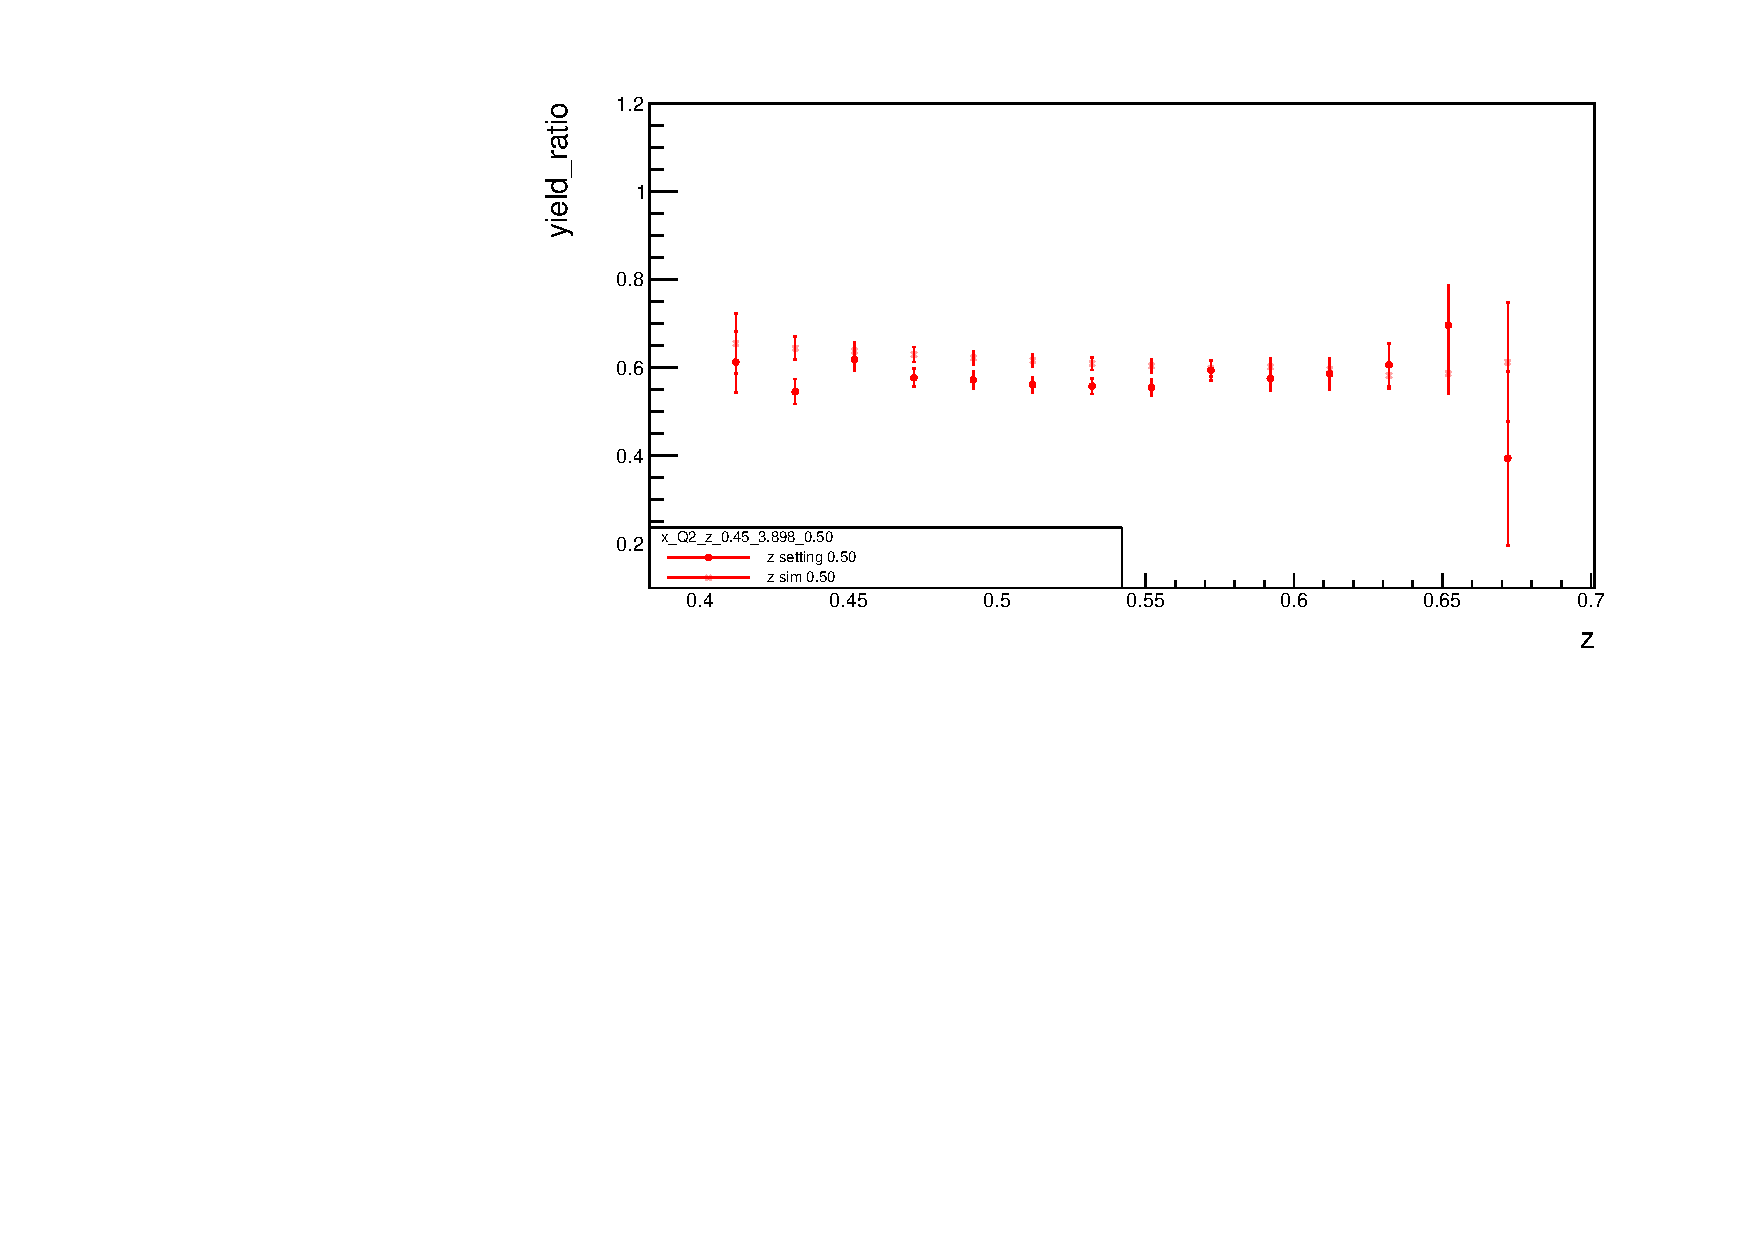
\includegraphics[width = 0.9\textwidth]{results/yield/statistics/x_Q2_z_0.45_3.898_0.50_ratio.pdf}
\end{column}
\end{columns}
\begin{columns}
\begin{column}[T]{0.5\textwidth}
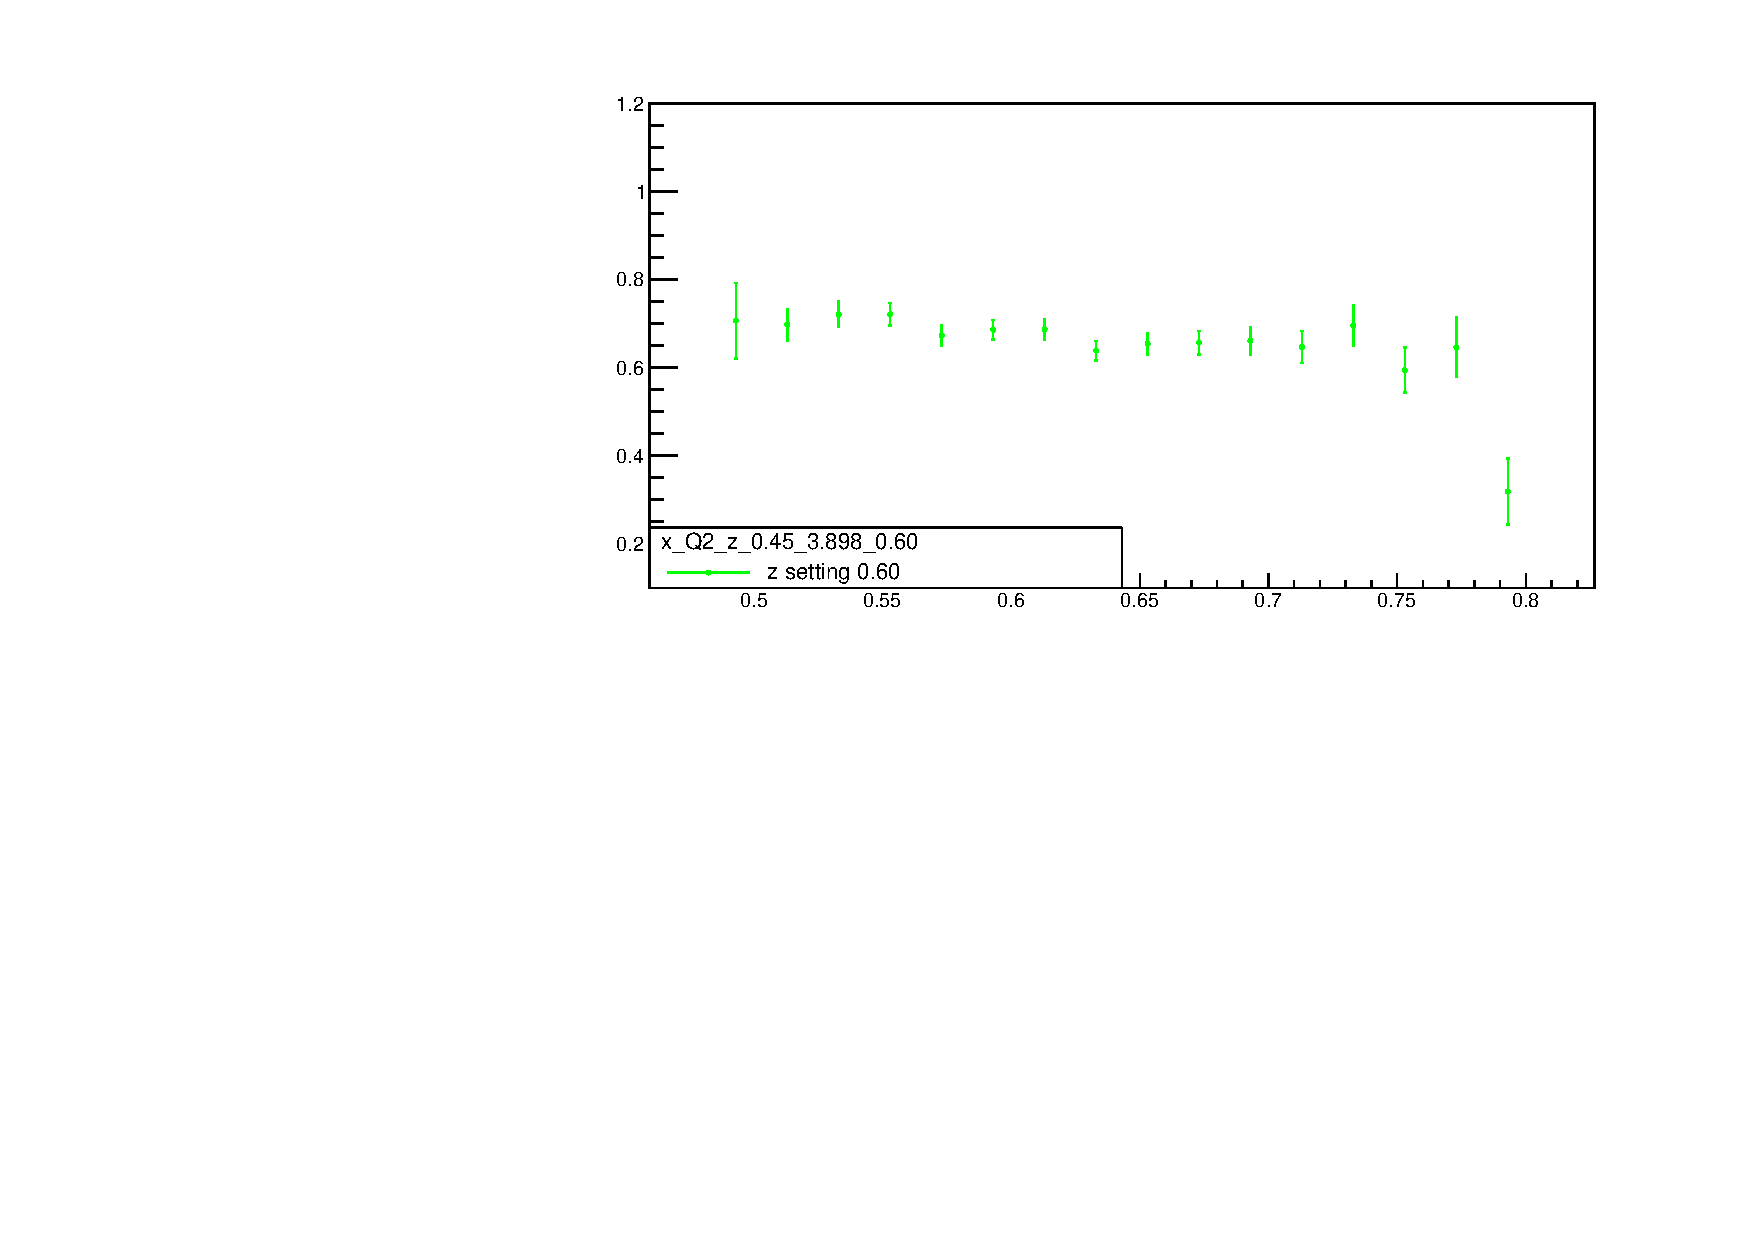
\includegraphics[width = 0.9\textwidth]{results/yield/statistics/x_Q2_z_0.45_3.898_0.60_ratio.pdf}
\end{column}
\begin{column}[T]{0.5\textwidth}
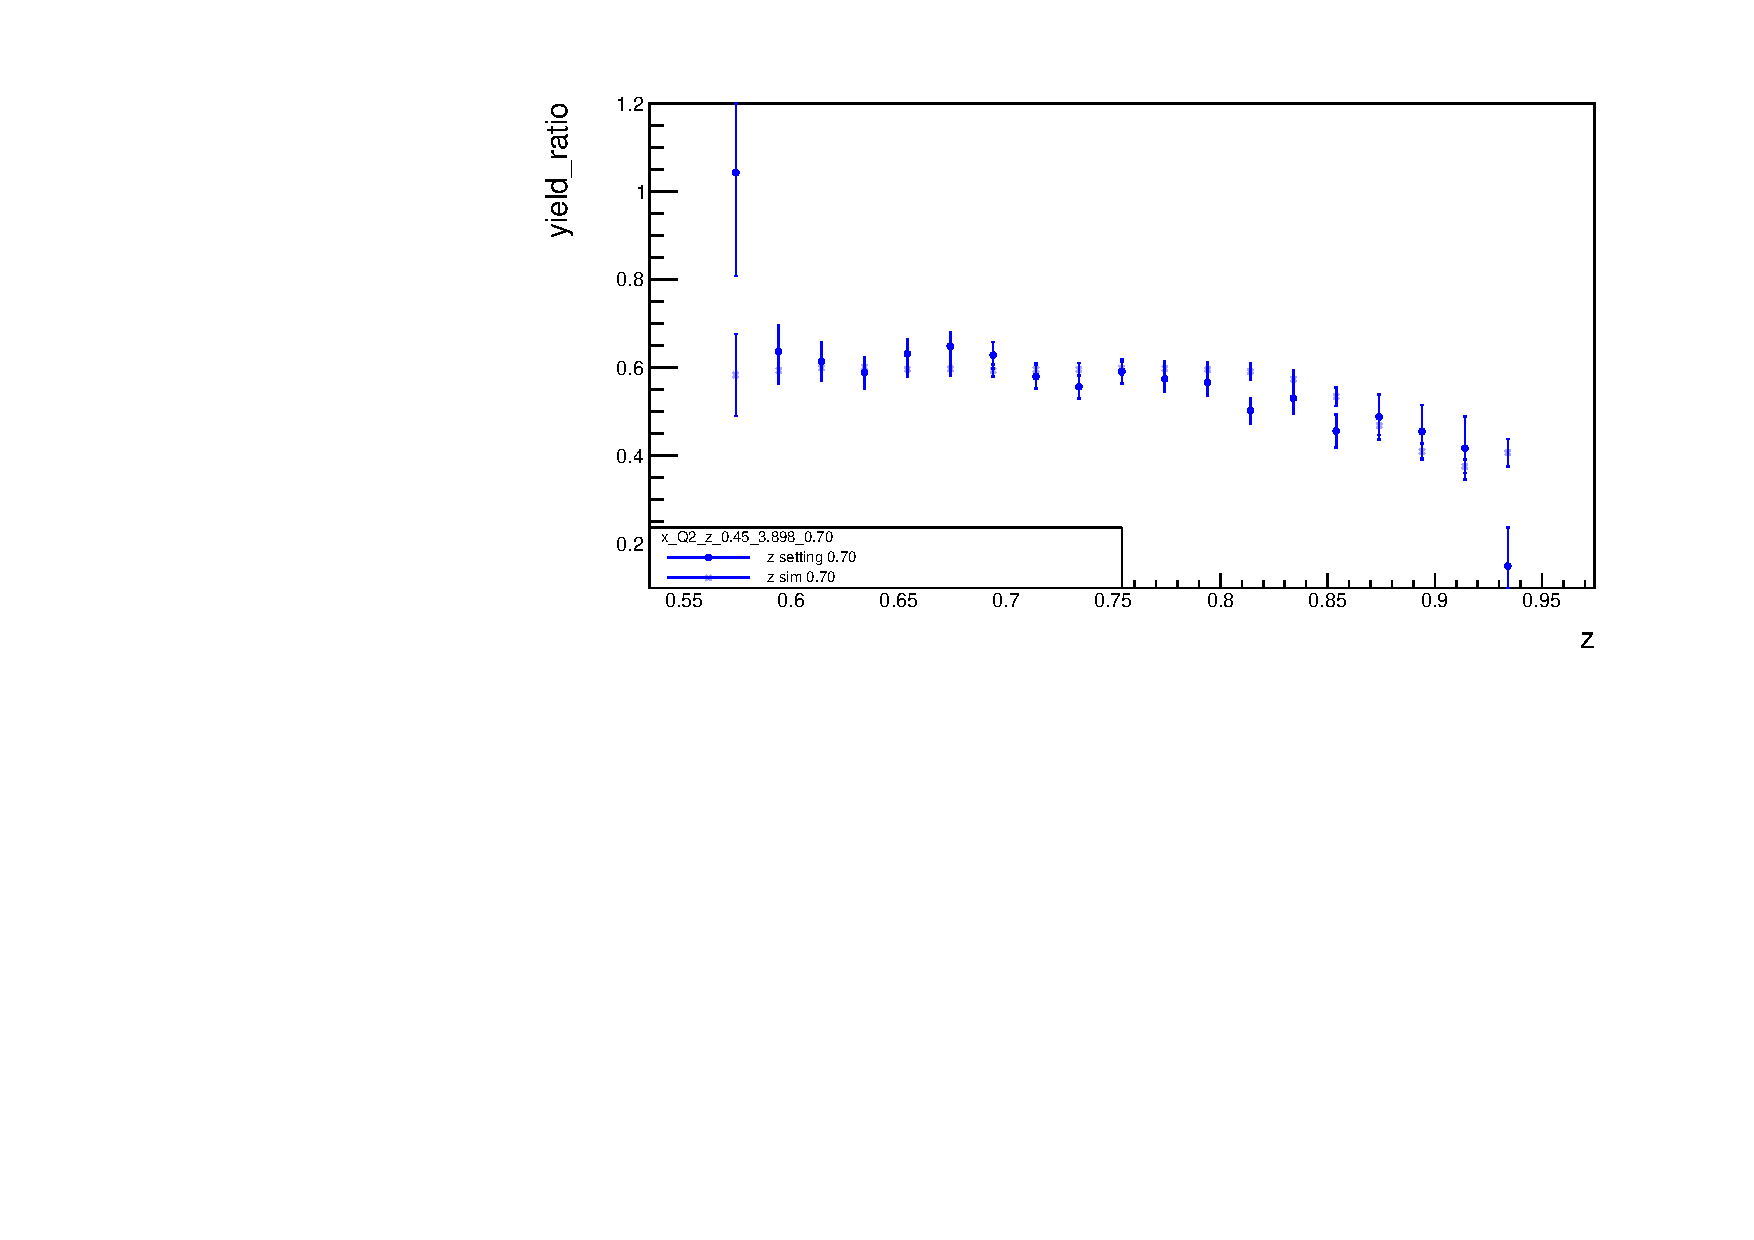
\includegraphics[width = 0.9\textwidth]{results/yield/statistics/x_Q2_z_0.45_3.898_0.70_ratio.pdf}
\end{column}
\end{columns}
\end{frame}
\begin{frame}{TE,pi eff, pi purity corrected yield ratio}
\begin{columns}
\begin{column}[T]{0.5\textwidth}
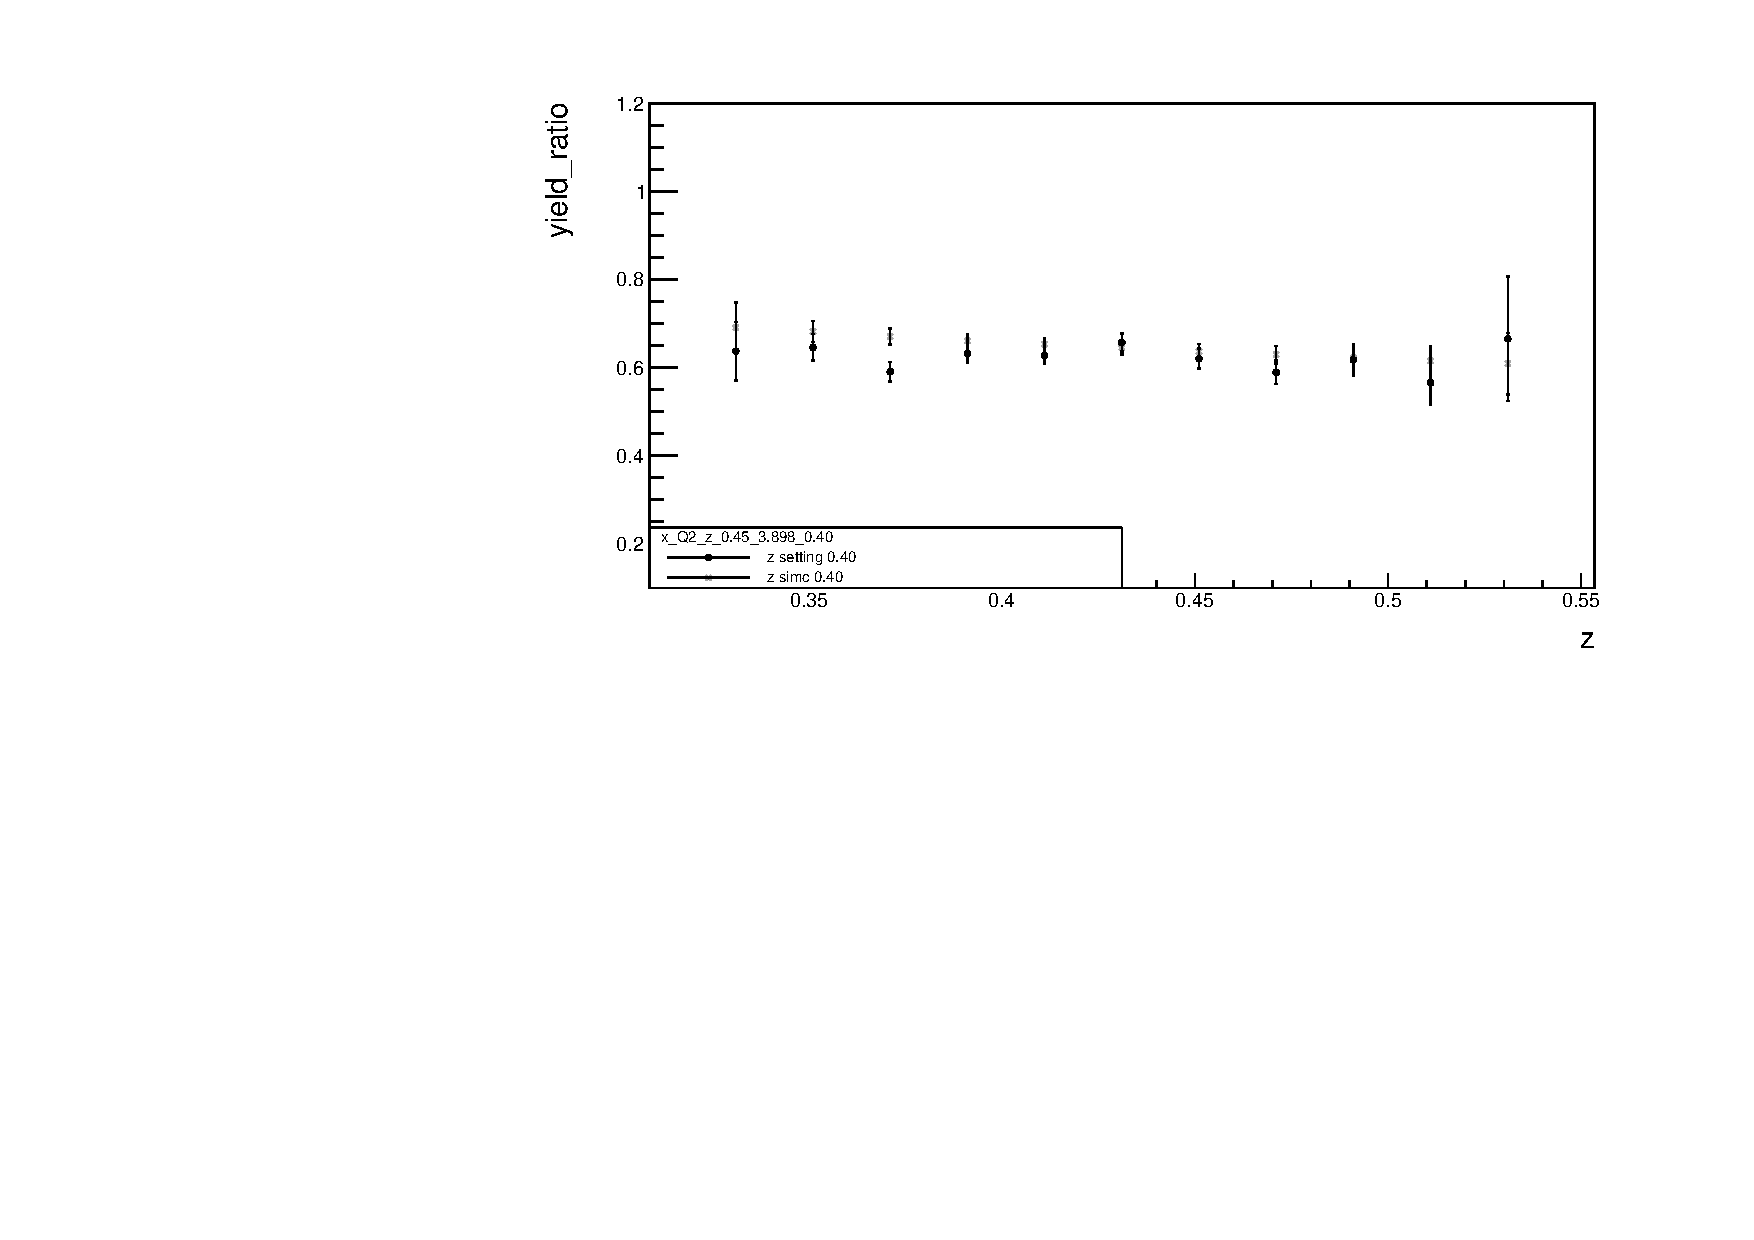
\includegraphics[width = 0.9\textwidth]{results/yield/statistics_corr/x_Q2_z_0.45_3.898_0.40_ratio.pdf}
\end{column}
\begin{column}[T]{0.5\textwidth}
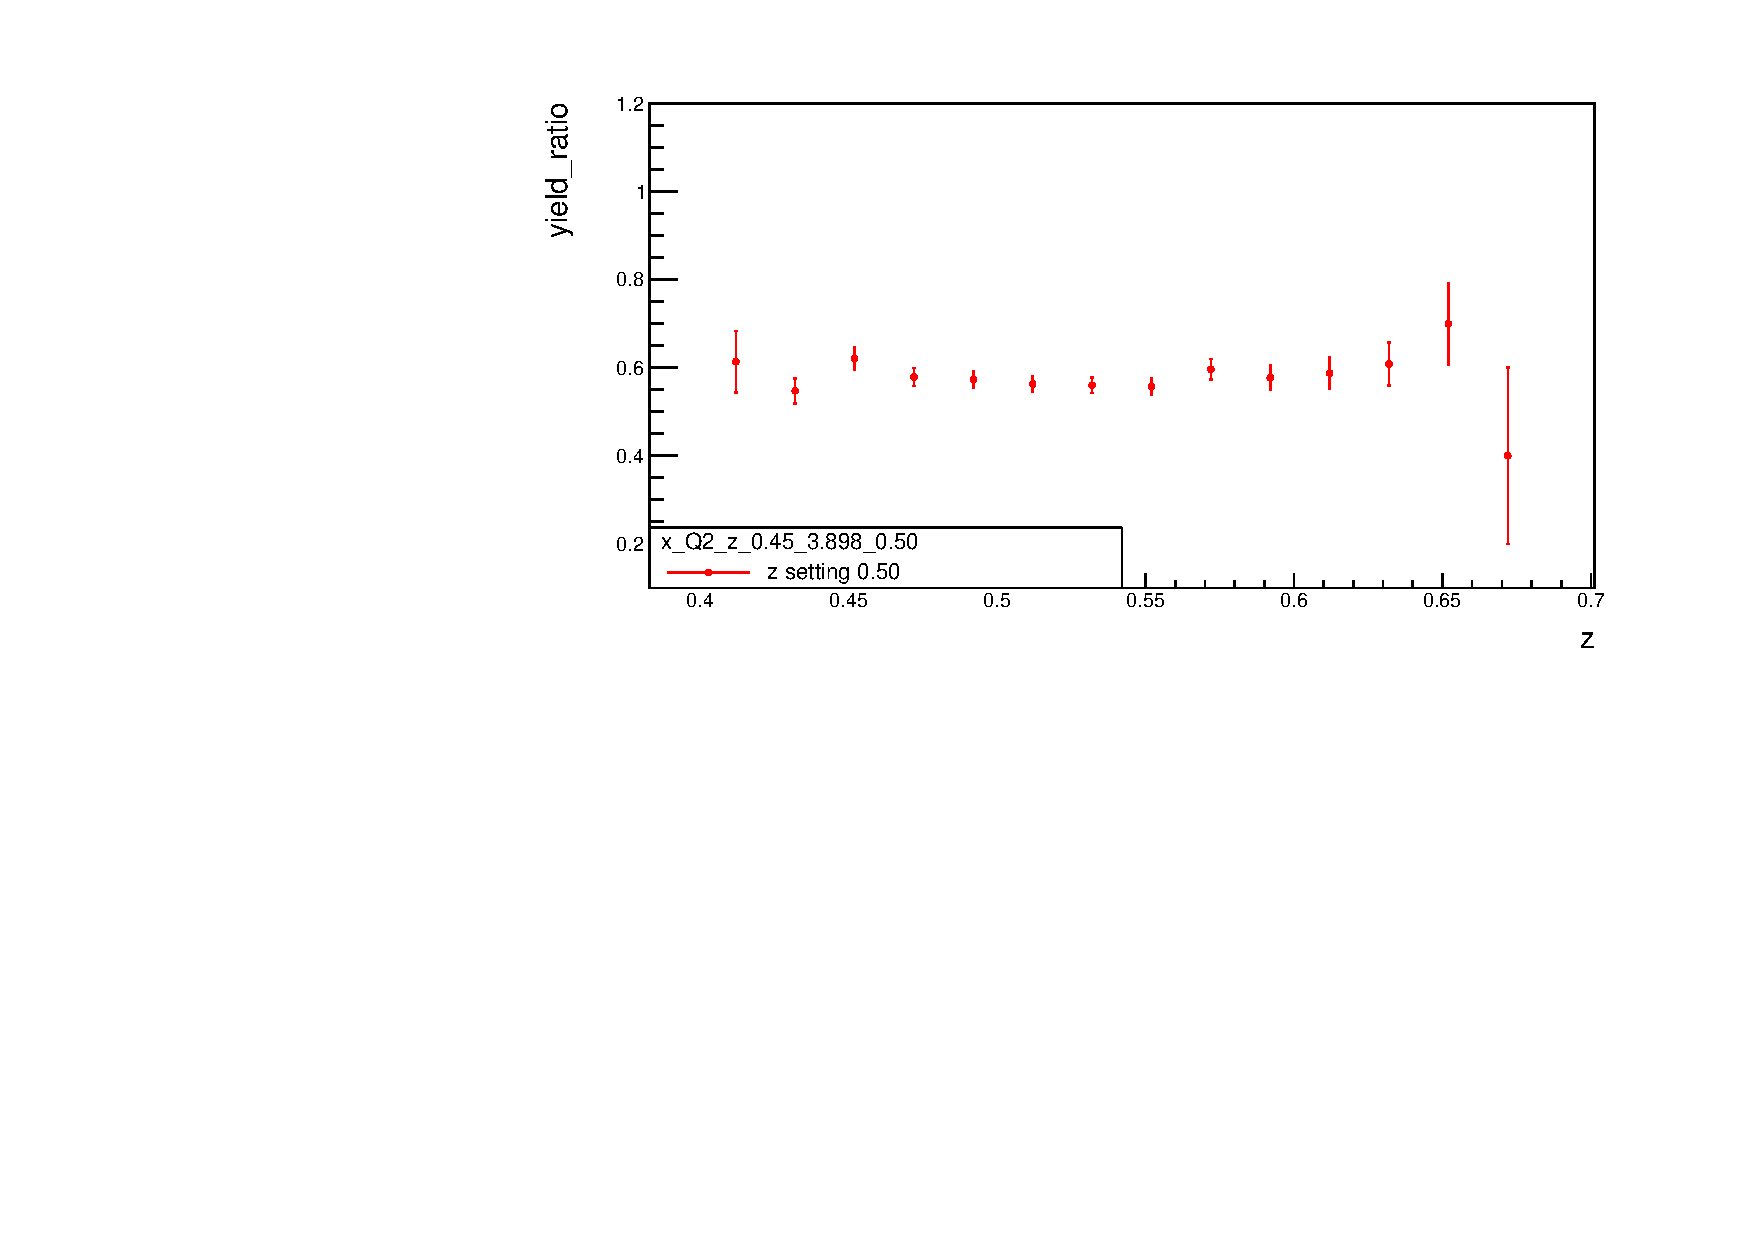
\includegraphics[width = 0.9\textwidth]{results/yield/statistics_corr/x_Q2_z_0.45_3.898_0.50_ratio.pdf}
\end{column}
\end{columns}
\begin{columns}
\begin{column}[T]{0.5\textwidth}
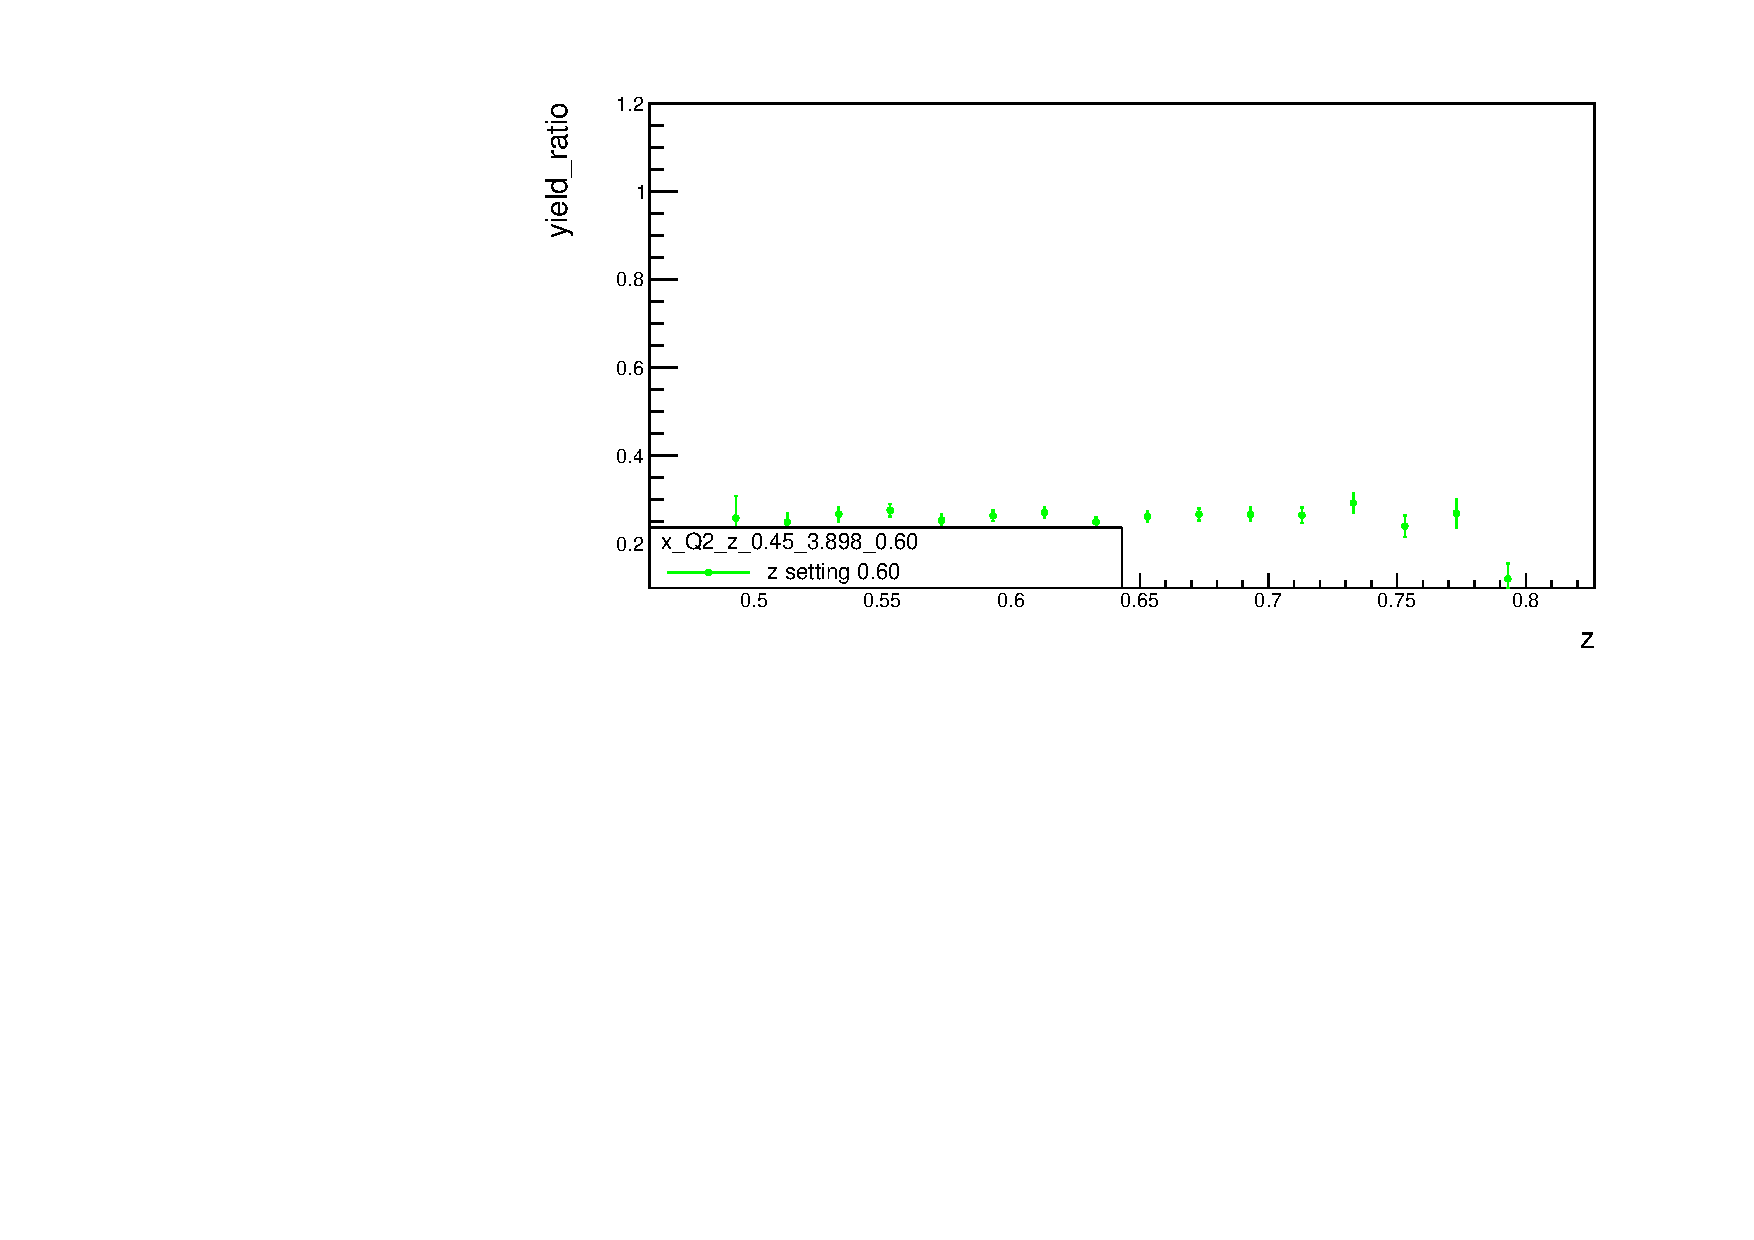
\includegraphics[width = 0.9\textwidth]{results/yield/statistics_corr/x_Q2_z_0.45_3.898_0.60_ratio.pdf}
\end{column}
\begin{column}[T]{0.5\textwidth}
\includegraphics[width = 0.9\textwidth]{results/yield/statistics_corr/x_Q2_z_0.45_3.898_0.70_ratio.pdf}
\end{column}
\end{columns}
\end{frame}
\begin{frame}{raw yield ratio}
\includegraphics[width = 0.9\textwidth]{results/yield/statistics/x_Q2_0.45_3.898_ratio.pdf}
\end{frame}
\begin{frame}{TE,pi eff, pi purity corrected yield ratio}
\includegraphics[width = 0.9\textwidth]{results/yield/statistics_corr/x_Q2_0.45_3.898_ratio.pdf}
\end{frame}
\begin{frame}{corrected yield}
\begin{columns}
\begin{column}[T]{0.25\textwidth}
\includegraphics[width = \textwidth]{results/yield/statistics_corr/yield_x_Q2_z_0.45_4.750_0.40_pos.png}
\end{column}
\begin{column}[T]{0.25\textwidth}
\includegraphics[width = \textwidth]{results/yield/statistics_corr/yield_x_Q2_z_0.45_4.750_0.40_neg.png}
\end{column}
\begin{column}[T]{0.25\textwidth}
\includegraphics[width = \textwidth]{results/yield/statistics_corr/yield_x_Q2_z_0.45_4.750_0.50_pos.png}
\end{column}
\begin{column}[T]{0.25\textwidth}
\includegraphics[width = \textwidth]{results/yield/statistics_corr/yield_x_Q2_z_0.45_4.750_0.50_neg.png}
\end{column}
\end{columns}
\begin{columns}
\begin{column}[T]{0.25\textwidth}
\includegraphics[width = \textwidth]{results/yield/statistics_corr/yield_x_Q2_z_0.45_4.750_0.60_pos.png}
\end{column}
\begin{column}[T]{0.25\textwidth}
\includegraphics[width = \textwidth]{results/yield/statistics_corr/yield_x_Q2_z_0.45_4.750_0.60_neg.png}
\end{column}
\begin{column}[T]{0.25\textwidth}
\includegraphics[width = \textwidth]{results/yield/statistics_corr/yield_x_Q2_z_0.45_4.750_0.70_pos.png}
\end{column}
\begin{column}[T]{0.25\textwidth}
\includegraphics[width = \textwidth]{results/yield/statistics_corr/yield_x_Q2_z_0.45_4.750_0.70_neg.png}
\end{column}
\end{columns}
\end{frame}
\begin{frame}{raw yield ratio}
\begin{columns}
\begin{column}[T]{0.5\textwidth}
\includegraphics[width = 0.9\textwidth]{results/yield/statistics/x_Q2_z_0.45_4.750_0.40_ratio.pdf}
\end{column}
\begin{column}[T]{0.5\textwidth}
\includegraphics[width = 0.9\textwidth]{results/yield/statistics/x_Q2_z_0.45_4.750_0.50_ratio.pdf}
\end{column}
\end{columns}
\begin{columns}
\begin{column}[T]{0.5\textwidth}
\includegraphics[width = 0.9\textwidth]{results/yield/statistics/x_Q2_z_0.45_4.750_0.60_ratio.pdf}
\end{column}
\begin{column}[T]{0.5\textwidth}
\includegraphics[width = 0.9\textwidth]{results/yield/statistics/x_Q2_z_0.45_4.750_0.70_ratio.pdf}
\end{column}
\end{columns}
\end{frame}
\begin{frame}{TE,pi eff, pi purity corrected yield ratio}
\begin{columns}
\begin{column}[T]{0.5\textwidth}
\includegraphics[width = 0.9\textwidth]{results/yield/statistics_corr/x_Q2_z_0.45_4.750_0.40_ratio.pdf}
\end{column}
\begin{column}[T]{0.5\textwidth}
\includegraphics[width = 0.9\textwidth]{results/yield/statistics_corr/x_Q2_z_0.45_4.750_0.50_ratio.pdf}
\end{column}
\end{columns}
\begin{columns}
\begin{column}[T]{0.5\textwidth}
\includegraphics[width = 0.9\textwidth]{results/yield/statistics_corr/x_Q2_z_0.45_4.750_0.60_ratio.pdf}
\end{column}
\begin{column}[T]{0.5\textwidth}
\includegraphics[width = 0.9\textwidth]{results/yield/statistics_corr/x_Q2_z_0.45_4.750_0.70_ratio.pdf}
\end{column}
\end{columns}
\end{frame}
\begin{frame}{raw yield ratio}
\includegraphics[width = 0.9\textwidth]{results/yield/statistics/x_Q2_0.45_4.750_ratio.pdf}
\end{frame}
\begin{frame}{TE,pi eff, pi purity corrected yield ratio}
\includegraphics[width = 0.9\textwidth]{results/yield/statistics_corr/x_Q2_0.45_4.750_ratio.pdf}
\end{frame}
\begin{frame}{corrected yield}
\begin{columns}
\begin{column}[T]{0.25\textwidth}
\includegraphics[width = \textwidth]{results/yield/statistics_corr/yield_x_Q2_z_0.50_3.979_0.40_pos.png}
\end{column}
\begin{column}[T]{0.25\textwidth}
\includegraphics[width = \textwidth]{results/yield/statistics_corr/yield_x_Q2_z_0.50_3.979_0.40_neg.png}
\end{column}
\begin{column}[T]{0.25\textwidth}
\includegraphics[width = \textwidth]{results/yield/statistics_corr/yield_x_Q2_z_0.50_3.979_0.50_pos.png}
\end{column}
\begin{column}[T]{0.25\textwidth}
\includegraphics[width = \textwidth]{results/yield/statistics_corr/yield_x_Q2_z_0.50_3.979_0.50_neg.png}
\end{column}
\end{columns}
\begin{columns}
\begin{column}[T]{0.25\textwidth}
\includegraphics[width = \textwidth]{results/yield/statistics_corr/yield_x_Q2_z_0.50_3.979_0.60_pos.png}
\end{column}
\begin{column}[T]{0.25\textwidth}
\includegraphics[width = \textwidth]{results/yield/statistics_corr/yield_x_Q2_z_0.50_3.979_0.60_neg.png}
\end{column}
\begin{column}[T]{0.25\textwidth}
\includegraphics[width = \textwidth]{results/yield/statistics_corr/yield_x_Q2_z_0.50_3.979_0.70_pos.png}
\end{column}
\begin{column}[T]{0.25\textwidth}
\includegraphics[width = \textwidth]{results/yield/statistics_corr/yield_x_Q2_z_0.50_3.979_0.70_neg.png}
\end{column}
\end{columns}
\end{frame}
\begin{frame}{raw yield ratio}
\begin{columns}
\begin{column}[T]{0.5\textwidth}
\includegraphics[width = 0.9\textwidth]{results/yield/statistics/x_Q2_z_0.50_3.979_0.40_ratio.pdf}
\end{column}
\begin{column}[T]{0.5\textwidth}
\includegraphics[width = 0.9\textwidth]{results/yield/statistics/x_Q2_z_0.50_3.979_0.50_ratio.pdf}
\end{column}
\end{columns}
\begin{columns}
\begin{column}[T]{0.5\textwidth}
\includegraphics[width = 0.9\textwidth]{results/yield/statistics/x_Q2_z_0.50_3.979_0.60_ratio.pdf}
\end{column}
\begin{column}[T]{0.5\textwidth}
\includegraphics[width = 0.9\textwidth]{results/yield/statistics/x_Q2_z_0.50_3.979_0.70_ratio.pdf}
\end{column}
\end{columns}
\end{frame}
\begin{frame}{TE,pi eff, pi purity corrected yield ratio}
\begin{columns}
\begin{column}[T]{0.5\textwidth}
\includegraphics[width = 0.9\textwidth]{results/yield/statistics_corr/x_Q2_z_0.50_3.979_0.40_ratio.pdf}
\end{column}
\begin{column}[T]{0.5\textwidth}
\includegraphics[width = 0.9\textwidth]{results/yield/statistics_corr/x_Q2_z_0.50_3.979_0.50_ratio.pdf}
\end{column}
\end{columns}
\begin{columns}
\begin{column}[T]{0.5\textwidth}
\includegraphics[width = 0.9\textwidth]{results/yield/statistics_corr/x_Q2_z_0.50_3.979_0.60_ratio.pdf}
\end{column}
\begin{column}[T]{0.5\textwidth}
\includegraphics[width = 0.9\textwidth]{results/yield/statistics_corr/x_Q2_z_0.50_3.979_0.70_ratio.pdf}
\end{column}
\end{columns}
\end{frame}
\begin{frame}{raw yield ratio}
\includegraphics[width = 0.9\textwidth]{results/yield/statistics/x_Q2_0.50_3.979_ratio.pdf}
\end{frame}
\begin{frame}{TE,pi eff, pi purity corrected yield ratio}
\includegraphics[width = 0.9\textwidth]{results/yield/statistics_corr/x_Q2_0.50_3.979_ratio.pdf}
\end{frame}
\begin{frame}{corrected yield}
\begin{columns}
\begin{column}[T]{0.25\textwidth}
\includegraphics[width = \textwidth]{results/yield/statistics_corr/yield_x_Q2_z_0.50_5.000_0.40_pos.png}
\end{column}
\begin{column}[T]{0.25\textwidth}
\includegraphics[width = \textwidth]{results/yield/statistics_corr/yield_x_Q2_z_0.50_5.000_0.40_neg.png}
\end{column}
\begin{column}[T]{0.25\textwidth}
\includegraphics[width = \textwidth]{results/yield/statistics_corr/yield_x_Q2_z_0.50_5.000_0.50_pos.png}
\end{column}
\begin{column}[T]{0.25\textwidth}
\includegraphics[width = \textwidth]{results/yield/statistics_corr/yield_x_Q2_z_0.50_5.000_0.50_neg.png}
\end{column}
\end{columns}
\begin{columns}
\begin{column}[T]{0.25\textwidth}
\includegraphics[width = \textwidth]{results/yield/statistics_corr/yield_x_Q2_z_0.50_5.000_0.60_pos.png}
\end{column}
\begin{column}[T]{0.25\textwidth}
\includegraphics[width = \textwidth]{results/yield/statistics_corr/yield_x_Q2_z_0.50_5.000_0.60_neg.png}
\end{column}
\begin{column}[T]{0.25\textwidth}
\includegraphics[width = \textwidth]{results/yield/statistics_corr/yield_x_Q2_z_0.50_5.000_0.70_pos.png}
\end{column}
\begin{column}[T]{0.25\textwidth}
\includegraphics[width = \textwidth]{results/yield/statistics_corr/yield_x_Q2_z_0.50_5.000_0.70_neg.png}
\end{column}
\end{columns}
\end{frame}
\begin{frame}{raw yield ratio}
\begin{columns}
\begin{column}[T]{0.5\textwidth}
\includegraphics[width = 0.9\textwidth]{results/yield/statistics/x_Q2_z_0.50_5.000_0.40_ratio.pdf}
\end{column}
\begin{column}[T]{0.5\textwidth}
\includegraphics[width = 0.9\textwidth]{results/yield/statistics/x_Q2_z_0.50_5.000_0.50_ratio.pdf}
\end{column}
\end{columns}
\begin{columns}
\begin{column}[T]{0.5\textwidth}
\includegraphics[width = 0.9\textwidth]{results/yield/statistics/x_Q2_z_0.50_5.000_0.60_ratio.pdf}
\end{column}
\begin{column}[T]{0.5\textwidth}
\includegraphics[width = 0.9\textwidth]{results/yield/statistics/x_Q2_z_0.50_5.000_0.70_ratio.pdf}
\end{column}
\end{columns}
\end{frame}
\begin{frame}{TE,pi eff, pi purity corrected yield ratio}
\begin{columns}
\begin{column}[T]{0.5\textwidth}
\includegraphics[width = 0.9\textwidth]{results/yield/statistics_corr/x_Q2_z_0.50_5.000_0.40_ratio.pdf}
\end{column}
\begin{column}[T]{0.5\textwidth}
\includegraphics[width = 0.9\textwidth]{results/yield/statistics_corr/x_Q2_z_0.50_5.000_0.50_ratio.pdf}
\end{column}
\end{columns}
\begin{columns}
\begin{column}[T]{0.5\textwidth}
\includegraphics[width = 0.9\textwidth]{results/yield/statistics_corr/x_Q2_z_0.50_5.000_0.60_ratio.pdf}
\end{column}
\begin{column}[T]{0.5\textwidth}
\includegraphics[width = 0.9\textwidth]{results/yield/statistics_corr/x_Q2_z_0.50_5.000_0.70_ratio.pdf}
\end{column}
\end{columns}
\end{frame}
\begin{frame}{raw yield ratio}
\includegraphics[width = 0.9\textwidth]{results/yield/statistics/x_Q2_0.50_5.000_ratio.pdf}
\end{frame}
\begin{frame}{TE,pi eff, pi purity corrected yield ratio}
\includegraphics[width = 0.9\textwidth]{results/yield/statistics_corr/x_Q2_0.50_5.000_ratio.pdf}
\end{frame}
\begin{frame}{corrected yield}
\begin{columns}
\begin{column}[T]{0.25\textwidth}
\includegraphics[width = \textwidth]{results/yield/statistics_corr/yield_x_Q2_z_0.50_5.500_0.40_pos.png}
\end{column}
\begin{column}[T]{0.25\textwidth}
\includegraphics[width = \textwidth]{results/yield/statistics_corr/yield_x_Q2_z_0.50_5.500_0.40_neg.png}
\end{column}
\begin{column}[T]{0.25\textwidth}
\includegraphics[width = \textwidth]{results/yield/statistics_corr/yield_x_Q2_z_0.50_5.500_0.50_pos.png}
\end{column}
\begin{column}[T]{0.25\textwidth}
\includegraphics[width = \textwidth]{results/yield/statistics_corr/yield_x_Q2_z_0.50_5.500_0.50_neg.png}
\end{column}
\end{columns}
\begin{columns}
\begin{column}[T]{0.25\textwidth}
\includegraphics[width = \textwidth]{results/yield/statistics_corr/yield_x_Q2_z_0.50_5.500_0.60_pos.png}
\end{column}
\begin{column}[T]{0.25\textwidth}
\includegraphics[width = \textwidth]{results/yield/statistics_corr/yield_x_Q2_z_0.50_5.500_0.60_neg.png}
\end{column}
\begin{column}[T]{0.25\textwidth}
\includegraphics[width = \textwidth]{results/yield/statistics_corr/yield_x_Q2_z_0.50_5.500_0.70_pos.png}
\end{column}
\begin{column}[T]{0.25\textwidth}
\includegraphics[width = \textwidth]{results/yield/statistics_corr/yield_x_Q2_z_0.50_5.500_0.70_neg.png}
\end{column}
\end{columns}
\end{frame}
\begin{frame}{raw yield ratio}
\begin{columns}
\begin{column}[T]{0.5\textwidth}
\includegraphics[width = 0.9\textwidth]{results/yield/statistics/x_Q2_z_0.50_5.500_0.40_ratio.pdf}
\end{column}
\begin{column}[T]{0.5\textwidth}
\includegraphics[width = 0.9\textwidth]{results/yield/statistics/x_Q2_z_0.50_5.500_0.50_ratio.pdf}
\end{column}
\end{columns}
\begin{columns}
\begin{column}[T]{0.5\textwidth}
\includegraphics[width = 0.9\textwidth]{results/yield/statistics/x_Q2_z_0.50_5.500_0.60_ratio.pdf}
\end{column}
\begin{column}[T]{0.5\textwidth}
\includegraphics[width = 0.9\textwidth]{results/yield/statistics/x_Q2_z_0.50_5.500_0.70_ratio.pdf}
\end{column}
\end{columns}
\end{frame}
\begin{frame}{TE,pi eff, pi purity corrected yield ratio}
\begin{columns}
\begin{column}[T]{0.5\textwidth}
\includegraphics[width = 0.9\textwidth]{results/yield/statistics_corr/x_Q2_z_0.50_5.500_0.40_ratio.pdf}
\end{column}
\begin{column}[T]{0.5\textwidth}
\includegraphics[width = 0.9\textwidth]{results/yield/statistics_corr/x_Q2_z_0.50_5.500_0.50_ratio.pdf}
\end{column}
\end{columns}
\begin{columns}
\begin{column}[T]{0.5\textwidth}
\includegraphics[width = 0.9\textwidth]{results/yield/statistics_corr/x_Q2_z_0.50_5.500_0.60_ratio.pdf}
\end{column}
\begin{column}[T]{0.5\textwidth}
\includegraphics[width = 0.9\textwidth]{results/yield/statistics_corr/x_Q2_z_0.50_5.500_0.70_ratio.pdf}
\end{column}
\end{columns}
\end{frame}
\begin{frame}{raw yield ratio}
\includegraphics[width = 0.9\textwidth]{results/yield/statistics/x_Q2_0.50_5.500_ratio.pdf}
\end{frame}
\begin{frame}{TE,pi eff, pi purity corrected yield ratio}
\includegraphics[width = 0.9\textwidth]{results/yield/statistics_corr/x_Q2_0.50_5.500_ratio.pdf}
\end{frame}
\begin{frame}{corrected yield}
\begin{columns}
\begin{column}[T]{0.25\textwidth}
\includegraphics[width = \textwidth]{results/yield/statistics_corr/yield_x_Q2_z_0.55_4.764_0.40_pos.png}
\end{column}
\begin{column}[T]{0.25\textwidth}
\includegraphics[width = \textwidth]{results/yield/statistics_corr/yield_x_Q2_z_0.55_4.764_0.40_neg.png}
\end{column}
\begin{column}[T]{0.25\textwidth}
\includegraphics[width = \textwidth]{results/yield/statistics_corr/yield_x_Q2_z_0.55_4.764_0.50_pos.png}
\end{column}
\begin{column}[T]{0.25\textwidth}
\includegraphics[width = \textwidth]{results/yield/statistics_corr/yield_x_Q2_z_0.55_4.764_0.50_neg.png}
\end{column}
\end{columns}
\begin{columns}
\begin{column}[T]{0.25\textwidth}
\includegraphics[width = \textwidth]{results/yield/statistics_corr/yield_x_Q2_z_0.55_4.764_0.60_pos.png}
\end{column}
\begin{column}[T]{0.25\textwidth}
\includegraphics[width = \textwidth]{results/yield/statistics_corr/yield_x_Q2_z_0.55_4.764_0.60_neg.png}
\end{column}
\begin{column}[T]{0.25\textwidth}
\includegraphics[width = \textwidth]{results/yield/statistics_corr/yield_x_Q2_z_0.55_4.764_0.70_pos.png}
\end{column}
\begin{column}[T]{0.25\textwidth}
\includegraphics[width = \textwidth]{results/yield/statistics_corr/yield_x_Q2_z_0.55_4.764_0.70_neg.png}
\end{column}
\end{columns}
\end{frame}
\begin{frame}{raw yield ratio}
\begin{columns}
\begin{column}[T]{0.5\textwidth}
\includegraphics[width = 0.9\textwidth]{results/yield/statistics/x_Q2_z_0.55_4.764_0.40_ratio.pdf}
\end{column}
\begin{column}[T]{0.5\textwidth}
\includegraphics[width = 0.9\textwidth]{results/yield/statistics/x_Q2_z_0.55_4.764_0.50_ratio.pdf}
\end{column}
\end{columns}
\begin{columns}
\begin{column}[T]{0.5\textwidth}
\includegraphics[width = 0.9\textwidth]{results/yield/statistics/x_Q2_z_0.55_4.764_0.60_ratio.pdf}
\end{column}
\begin{column}[T]{0.5\textwidth}
\includegraphics[width = 0.9\textwidth]{results/yield/statistics/x_Q2_z_0.55_4.764_0.70_ratio.pdf}
\end{column}
\end{columns}
\end{frame}
\begin{frame}{TE,pi eff, pi purity corrected yield ratio}
\begin{columns}
\begin{column}[T]{0.5\textwidth}
\includegraphics[width = 0.9\textwidth]{results/yield/statistics_corr/x_Q2_z_0.55_4.764_0.40_ratio.pdf}
\end{column}
\begin{column}[T]{0.5\textwidth}
\includegraphics[width = 0.9\textwidth]{results/yield/statistics_corr/x_Q2_z_0.55_4.764_0.50_ratio.pdf}
\end{column}
\end{columns}
\begin{columns}
\begin{column}[T]{0.5\textwidth}
\includegraphics[width = 0.9\textwidth]{results/yield/statistics_corr/x_Q2_z_0.55_4.764_0.60_ratio.pdf}
\end{column}
\begin{column}[T]{0.5\textwidth}
\includegraphics[width = 0.9\textwidth]{results/yield/statistics_corr/x_Q2_z_0.55_4.764_0.70_ratio.pdf}
\end{column}
\end{columns}
\end{frame}
\begin{frame}{raw yield ratio}
\includegraphics[width = 0.9\textwidth]{results/yield/statistics/x_Q2_0.55_4.764_ratio.pdf}
\end{frame}
\begin{frame}{TE,pi eff, pi purity corrected yield ratio}
\includegraphics[width = 0.9\textwidth]{results/yield/statistics_corr/x_Q2_0.55_4.764_ratio.pdf}
\end{frame}
\begin{frame}{corrected yield}
\begin{columns}
\begin{column}[T]{0.25\textwidth}
\includegraphics[width = \textwidth]{results/yield/statistics_corr/yield_x_Q2_z_0.55_5.500_0.45_pos.png}
\end{column}
\begin{column}[T]{0.25\textwidth}
\includegraphics[width = \textwidth]{results/yield/statistics_corr/yield_x_Q2_z_0.55_5.500_0.45_neg.png}
\end{column}
\begin{column}[T]{0.25\textwidth}
\includegraphics[width = \textwidth]{results/yield/statistics_corr/yield_x_Q2_z_0.55_5.500_0.55_pos.png}
\end{column}
\begin{column}[T]{0.25\textwidth}
\includegraphics[width = \textwidth]{results/yield/statistics_corr/yield_x_Q2_z_0.55_5.500_0.55_neg.png}
\end{column}
\end{columns}
\begin{columns}
\begin{column}[T]{0.25\textwidth}
\includegraphics[width = \textwidth]{results/yield/statistics_corr/yield_x_Q2_z_0.55_5.500_0.65_pos.png}
\end{column}
\begin{column}[T]{0.25\textwidth}
\includegraphics[width = \textwidth]{results/yield/statistics_corr/yield_x_Q2_z_0.55_5.500_0.65_neg.png}
\end{column}
\end{frame}
\begin{frame}{raw yield ratio}
\begin{columns}
\begin{column}[T]{0.5\textwidth}
\includegraphics[width = 0.9\textwidth]{results/yield/statistics/x_Q2_z_0.55_5.500_0.45_ratio.pdf}
\end{column}
\begin{column}[T]{0.5\textwidth}
\includegraphics[width = 0.9\textwidth]{results/yield/statistics/x_Q2_z_0.55_5.500_0.55_ratio.pdf}
\end{column}
\end{columns}
\begin{columns}
\begin{column}[T]{0.5\textwidth}
\includegraphics[width = 0.9\textwidth]{results/yield/statistics/x_Q2_z_0.55_5.500_0.65_ratio.pdf}
\end{column}
\begin{column}[T]{0.5\textwidth}
\end{column}
\end{columns}
\end{frame}
\begin{frame}{TE,pi eff, pi purity corrected yield ratio}
\begin{columns}
\begin{column}[T]{0.5\textwidth}
\includegraphics[width = 0.9\textwidth]{results/yield/statistics_corr/x_Q2_z_0.55_5.500_0.45_ratio.pdf}
\end{column}
\begin{column}[T]{0.5\textwidth}
\includegraphics[width = 0.9\textwidth]{results/yield/statistics_corr/x_Q2_z_0.55_5.500_0.55_ratio.pdf}
\end{column}
\end{columns}
\begin{columns}
\begin{column}[T]{0.5\textwidth}
\includegraphics[width = 0.9\textwidth]{results/yield/statistics_corr/x_Q2_z_0.55_5.500_0.65_ratio.pdf}
\end{column}
\begin{column}[T]{0.5\textwidth}
\end{column}
\end{columns}
\end{frame}
\begin{frame}{raw yield ratio}
\includegraphics[width = 0.9\textwidth]{results/yield/statistics/x_Q2_0.55_5.500_ratio.pdf}
\end{frame}
\begin{frame}{TE,pi eff, pi purity corrected yield ratio}
\includegraphics[width = 0.9\textwidth]{results/yield/statistics_corr/x_Q2_0.55_5.500_ratio.pdf}
\end{frame}
\begin{frame}{corrected yield}
\begin{columns}
\begin{column}[T]{0.25\textwidth}
\includegraphics[width = \textwidth]{results/yield/statistics_corr/yield_x_Q2_z_0.60_4.775_0.40_pos.png}
\end{column}
\begin{column}[T]{0.25\textwidth}
\includegraphics[width = \textwidth]{results/yield/statistics_corr/yield_x_Q2_z_0.60_4.775_0.40_neg.png}
\end{column}
\begin{column}[T]{0.25\textwidth}
\includegraphics[width = \textwidth]{results/yield/statistics_corr/yield_x_Q2_z_0.60_4.775_0.50_pos.png}
\end{column}
\begin{column}[T]{0.25\textwidth}
\includegraphics[width = \textwidth]{results/yield/statistics_corr/yield_x_Q2_z_0.60_4.775_0.50_neg.png}
\end{column}
\end{columns}
\begin{columns}
\begin{column}[T]{0.25\textwidth}
\includegraphics[width = \textwidth]{results/yield/statistics_corr/yield_x_Q2_z_0.60_4.775_0.60_pos.png}
\end{column}
\begin{column}[T]{0.25\textwidth}
\includegraphics[width = \textwidth]{results/yield/statistics_corr/yield_x_Q2_z_0.60_4.775_0.60_neg.png}
\end{column}
\begin{column}[T]{0.25\textwidth}
\includegraphics[width = \textwidth]{results/yield/statistics_corr/yield_x_Q2_z_0.60_4.775_0.70_pos.png}
\end{column}
\begin{column}[T]{0.25\textwidth}
\includegraphics[width = \textwidth]{results/yield/statistics_corr/yield_x_Q2_z_0.60_4.775_0.70_neg.png}
\end{column}
\end{columns}
\end{frame}
\begin{frame}{raw yield ratio}
\begin{columns}
\begin{column}[T]{0.5\textwidth}
\includegraphics[width = 0.9\textwidth]{results/yield/statistics/x_Q2_z_0.60_4.775_0.40_ratio.pdf}
\end{column}
\begin{column}[T]{0.5\textwidth}
\includegraphics[width = 0.9\textwidth]{results/yield/statistics/x_Q2_z_0.60_4.775_0.50_ratio.pdf}
\end{column}
\end{columns}
\begin{columns}
\begin{column}[T]{0.5\textwidth}
\includegraphics[width = 0.9\textwidth]{results/yield/statistics/x_Q2_z_0.60_4.775_0.60_ratio.pdf}
\end{column}
\begin{column}[T]{0.5\textwidth}
\includegraphics[width = 0.9\textwidth]{results/yield/statistics/x_Q2_z_0.60_4.775_0.70_ratio.pdf}
\end{column}
\end{columns}
\end{frame}
\begin{frame}{TE,pi eff, pi purity corrected yield ratio}
\begin{columns}
\begin{column}[T]{0.5\textwidth}
\includegraphics[width = 0.9\textwidth]{results/yield/statistics_corr/x_Q2_z_0.60_4.775_0.40_ratio.pdf}
\end{column}
\begin{column}[T]{0.5\textwidth}
\includegraphics[width = 0.9\textwidth]{results/yield/statistics_corr/x_Q2_z_0.60_4.775_0.50_ratio.pdf}
\end{column}
\end{columns}
\begin{columns}
\begin{column}[T]{0.5\textwidth}
\includegraphics[width = 0.9\textwidth]{results/yield/statistics_corr/x_Q2_z_0.60_4.775_0.60_ratio.pdf}
\end{column}
\begin{column}[T]{0.5\textwidth}
\includegraphics[width = 0.9\textwidth]{results/yield/statistics_corr/x_Q2_z_0.60_4.775_0.70_ratio.pdf}
\end{column}
\end{columns}
\end{frame}
\begin{frame}{raw yield ratio}
\includegraphics[width = 0.9\textwidth]{results/yield/statistics/x_Q2_0.60_4.775_ratio.pdf}
\end{frame}
\begin{frame}{TE,pi eff, pi purity corrected yield ratio}
\includegraphics[width = 0.9\textwidth]{results/yield/statistics_corr/x_Q2_0.60_4.775_ratio.pdf}
\end{frame}
\begin{frame}{corrected yield}
\begin{columns}
\begin{column}[T]{0.25\textwidth}
\includegraphics[width = \textwidth]{results/yield/statistics_corr/yield_x_Q2_z_0.60_5.500_0.45_pos.png}
\end{column}
\begin{column}[T]{0.25\textwidth}
\includegraphics[width = \textwidth]{results/yield/statistics_corr/yield_x_Q2_z_0.60_5.500_0.45_neg.png}
\end{column}
\begin{column}[T]{0.25\textwidth}
\includegraphics[width = \textwidth]{results/yield/statistics_corr/yield_x_Q2_z_0.60_5.500_0.55_pos.png}
\end{column}
\begin{column}[T]{0.25\textwidth}
\includegraphics[width = \textwidth]{results/yield/statistics_corr/yield_x_Q2_z_0.60_5.500_0.55_neg.png}
\end{column}
\end{columns}
\begin{columns}
\begin{column}[T]{0.25\textwidth}
\includegraphics[width = \textwidth]{results/yield/statistics_corr/yield_x_Q2_z_0.60_5.500_0.65_pos.png}
\end{column}
\begin{column}[T]{0.25\textwidth}
\includegraphics[width = \textwidth]{results/yield/statistics_corr/yield_x_Q2_z_0.60_5.500_0.65_neg.png}
\end{column}
\begin{column}[T]{0.25\textwidth}
\includegraphics[width = \textwidth]{results/yield/statistics_corr/yield_x_Q2_z_0.60_5.500_0.90_pos.png}
\end{column}
\begin{column}[T]{0.25\textwidth}
\includegraphics[width = \textwidth]{results/yield/statistics_corr/yield_x_Q2_z_0.60_5.500_0.90_neg.png}
\end{column}
\end{columns}
\end{frame}
\begin{frame}{raw yield ratio}
\begin{columns}
\begin{column}[T]{0.5\textwidth}
\includegraphics[width = 0.9\textwidth]{results/yield/statistics/x_Q2_z_0.60_5.500_0.45_ratio.pdf}
\end{column}
\begin{column}[T]{0.5\textwidth}
\includegraphics[width = 0.9\textwidth]{results/yield/statistics/x_Q2_z_0.60_5.500_0.55_ratio.pdf}
\end{column}
\end{columns}
\begin{columns}
\begin{column}[T]{0.5\textwidth}
\includegraphics[width = 0.9\textwidth]{results/yield/statistics/x_Q2_z_0.60_5.500_0.65_ratio.pdf}
\end{column}
\begin{column}[T]{0.5\textwidth}
\includegraphics[width = 0.9\textwidth]{results/yield/statistics/x_Q2_z_0.60_5.500_0.90_ratio.pdf}
\end{column}
\end{columns}
\end{frame}
\begin{frame}{TE,pi eff, pi purity corrected yield ratio}
\begin{columns}
\begin{column}[T]{0.5\textwidth}
\includegraphics[width = 0.9\textwidth]{results/yield/statistics_corr/x_Q2_z_0.60_5.500_0.45_ratio.pdf}
\end{column}
\begin{column}[T]{0.5\textwidth}
\includegraphics[width = 0.9\textwidth]{results/yield/statistics_corr/x_Q2_z_0.60_5.500_0.55_ratio.pdf}
\end{column}
\end{columns}
\begin{columns}
\begin{column}[T]{0.5\textwidth}
\includegraphics[width = 0.9\textwidth]{results/yield/statistics_corr/x_Q2_z_0.60_5.500_0.65_ratio.pdf}
\end{column}
\begin{column}[T]{0.5\textwidth}
\includegraphics[width = 0.9\textwidth]{results/yield/statistics_corr/x_Q2_z_0.60_5.500_0.90_ratio.pdf}
\end{column}
\end{columns}
\end{frame}
\begin{frame}{raw yield ratio}
\includegraphics[width = 0.9\textwidth]{results/yield/statistics/x_Q2_0.60_5.500_ratio.pdf}
\end{frame}
\begin{frame}{TE,pi eff, pi purity corrected yield ratio}
\includegraphics[width = 0.9\textwidth]{results/yield/statistics_corr/x_Q2_0.60_5.500_ratio.pdf}
\end{frame}
\begin{frame}{corrected yield}
\begin{columns}
\begin{column}[T]{0.25\textwidth}
\includegraphics[width = \textwidth]{results/yield/statistics_corr/yield_x_Q2_z_0.65_5.500_0.40_pos.png}
\end{column}
\begin{column}[T]{0.25\textwidth}
\includegraphics[width = \textwidth]{results/yield/statistics_corr/yield_x_Q2_z_0.65_5.500_0.40_neg.png}
\end{column}
\begin{column}[T]{0.25\textwidth}
\includegraphics[width = \textwidth]{results/yield/statistics_corr/yield_x_Q2_z_0.65_5.500_0.50_pos.png}
\end{column}
\begin{column}[T]{0.25\textwidth}
\includegraphics[width = \textwidth]{results/yield/statistics_corr/yield_x_Q2_z_0.65_5.500_0.50_neg.png}
\end{column}
\end{columns}
\begin{columns}
\begin{column}[T]{0.25\textwidth}
\includegraphics[width = \textwidth]{results/yield/statistics_corr/yield_x_Q2_z_0.65_5.500_0.60_pos.png}
\end{column}
\begin{column}[T]{0.25\textwidth}
\includegraphics[width = \textwidth]{results/yield/statistics_corr/yield_x_Q2_z_0.65_5.500_0.60_neg.png}
\end{column}
\begin{column}[T]{0.25\textwidth}
\includegraphics[width = \textwidth]{results/yield/statistics_corr/yield_x_Q2_z_0.65_5.500_0.70_pos.png}
\end{column}
\begin{column}[T]{0.25\textwidth}
\includegraphics[width = \textwidth]{results/yield/statistics_corr/yield_x_Q2_z_0.65_5.500_0.70_neg.png}
\end{column}
\end{columns}
\end{frame}
\begin{frame}{raw yield ratio}
\begin{columns}
\begin{column}[T]{0.5\textwidth}
\includegraphics[width = 0.9\textwidth]{results/yield/statistics/x_Q2_z_0.65_5.500_0.40_ratio.pdf}
\end{column}
\begin{column}[T]{0.5\textwidth}
\includegraphics[width = 0.9\textwidth]{results/yield/statistics/x_Q2_z_0.65_5.500_0.50_ratio.pdf}
\end{column}
\end{columns}
\begin{columns}
\begin{column}[T]{0.5\textwidth}
\includegraphics[width = 0.9\textwidth]{results/yield/statistics/x_Q2_z_0.65_5.500_0.60_ratio.pdf}
\end{column}
\begin{column}[T]{0.5\textwidth}
\includegraphics[width = 0.9\textwidth]{results/yield/statistics/x_Q2_z_0.65_5.500_0.70_ratio.pdf}
\end{column}
\end{columns}
\end{frame}
\begin{frame}{TE,pi eff, pi purity corrected yield ratio}
\begin{columns}
\begin{column}[T]{0.5\textwidth}
\includegraphics[width = 0.9\textwidth]{results/yield/statistics_corr/x_Q2_z_0.65_5.500_0.40_ratio.pdf}
\end{column}
\begin{column}[T]{0.5\textwidth}
\includegraphics[width = 0.9\textwidth]{results/yield/statistics_corr/x_Q2_z_0.65_5.500_0.50_ratio.pdf}
\end{column}
\end{columns}
\begin{columns}
\begin{column}[T]{0.5\textwidth}
\includegraphics[width = 0.9\textwidth]{results/yield/statistics_corr/x_Q2_z_0.65_5.500_0.60_ratio.pdf}
\end{column}
\begin{column}[T]{0.5\textwidth}
\includegraphics[width = 0.9\textwidth]{results/yield/statistics_corr/x_Q2_z_0.65_5.500_0.70_ratio.pdf}
\end{column}
\end{columns}
\end{frame}
\begin{frame}{raw yield ratio}
\includegraphics[width = 0.9\textwidth]{results/yield/statistics/x_Q2_0.65_5.500_ratio.pdf}
\end{frame}
\begin{frame}{TE,pi eff, pi purity corrected yield ratio}
\includegraphics[width = 0.9\textwidth]{results/yield/statistics_corr/x_Q2_0.65_5.500_ratio.pdf}
\end{frame}



\end{document}
 
